\documentclass[11pt,oneside]{uhthesis}
\usepackage{mathpazo}

\renewcommand{\tablename}{Tabla}
\title{Una propuesta para encontrar el sistema de ecuaciones diferenciales lineales en los parámetros que mejor ajuste un conjunto de datos}
\author{Enrique Martínez González}
\advisor{MSc. Fernando Rodríguez Flores}
\coadvisor{Lic. Ernesto Borrego Rodríguez}
\degree{Licenciado en Ciencias de la Computación}
\faculty{Facultad de Matemática y Computación}
\date{Diciembre de 2022}
\logo{Graphics/uhlogo}


\begin{document}
\selectlanguage{spanish}

\frontmatter
\maketitle

\begin{dedication}
    \textit{
        Hola que tal\\
        si, aquí va la dedicatoria y tal}
\end{dedication}
\chapter*{Agradecimientos}\label{chapter:agradecimientos}

A mi tutor Fernando Rodríguez, por dedicar su valisísimo tiempo y geniales ideas a la realización de este trabajo. Por guiarme durante todo este proceso y regalarme sus conocimientos y consejos.
\\

A Ernesto Borrego por aconsejarme tan fabuloso tutor y por su preocupación constante acerca del avance de la investigación.
\\

A David Guaty por su apoyo y gran habilidad en la solución de problemas matemáticos.
\\

A mi hermano Fernando en su enseñanza de buenas prácticas en la programación.
\\

A mi madre Elizabeth por su amor y dedicación en este trabajo.
\\

A Dianelys por acogerme como otro hijo durante esta etapa.
\\

A Diana por su apoyo incondicional.
\\

Al resto de mi familia por siempre estar presentes en mi vida apoyándome a seguir adelante.

\begin{opinion}
    Y aqui va la opinión del tutor :D

    \vspace{1cm}


    \begin{flushright}
        \underline{\hspace{6.5cm}}\\
        MSc. Fernando Raul Rodriguez Flores

        Facultad de Matemática y Computación

        Universidad de la Habana

        Noviembre, 2022
    \end{flushright}

\end{opinion}
\begin{abstract}

    Los sistemas de ecuaciones diferenciales ordinarias lineales con respecto a los parámetros se pueden utilizar para predecir y describir fenómenos de la naturaleza, la ciencia, la tecnología y la sociedad. Esta predicción se realiza mediante la generación de modelos matemáticos a partir de observaciones del fenómeno. La obtención del modelo permite analizar la relación entre las distintas variables y parámetros que ocurren en el fenómeno observado.

    Para encontrar de forma automática modelos que desriben un conjunto de datos se desarrollan diversos métodos que son capaces de plantear de forma simbólica los sistemas que describen los datos. Estos algoritmos utilizan el método de regresión simbólica. La problema de regresión simbólica en sistemas de ecuaciones diferenciales se puede resolver mediante el uso de algoritmos genéticos o redes neuronales.

    En este trabajo se propone una herramienta para encontrar el sistema de ecuaciones diferenciales lineales con respecto a los parámetros que mejor describa un conjunto de datos utlizando regresión simbólica mediante algoritmos genéticos. Se aproximan los parámetros presentes en el modelo mediante la solución de un sistema de ecuaciones lineales y en caso de que los datos presenten ruido se utiliza un spline de suavizado para la aproximación de los datos. El comportamiento de la herrmienta propuesta muestra la capacidad de generación de un sistema que describe los datos, incluso ante la presencia de ruido.


\end{abstract}

\begin{enabstract}

    Ordinary differential equations systems linear with respect to parameters can be used to predict and describe phenomena in nature, science, technology, and society. This prediction is made by generating mathematical models from observations of the phenomenon. Obtaining the model allows to analyze the relationship between the different variables and parameters that occur in the observed phenomenon.

    To automatically find models that describe a set of data, various methods are developed that are capable of symbolically posing the systems that describe the data. These algorithms use the symbolic regression method. The symbolic regression problem in systems of differential equations can be solved by using genetic algorithms or neural networks.

    In this work, a tool is proposed to find the oridnary differential equations system linear with respect to the parameters that best describes a data set using symbolic regression through genetic algorithms. The parameters present in the model are approximated by solving a linear equations system and in case the data present noise, a smoothing spline is used to approximate the data. The behavior of the proposed tool shows the generation capacity of a system that describes the data, even in the presence of noise.

\end{enabstract}
\tableofcontents
\listoffigures

\mainmatter

\chapter*{Introducción}\label{chapter:introduction}
\addcontentsline{toc}{chapter}{Introducción}

\qquad

La regresión es un conjunto de procesos estadísticos para estimar las relaciones entre una variable dependiente y una o más variables independientes. La forma más común de análisis de regresión es la regresión lineal, en la que se encuentra la línea o una combinación lineal más compleja que se ajusta más a los datos de acuerdo con un criterio matemático específico. Por ejemplo, el método de los mínimos cuadrados ordinarios calcula el único hiperplano que minimiza la suma de las diferencias al cuadrado entre los datos dados y ese hiperplano. Por razones matemáticas específicas, esto le permite al investigador estimar la variable dependiente cuando las variables independientes toman un conjunto dado de valores.

El análisis de regresión se utiliza principalmente para dos propósitos conceptualmente distintos.

\begin{itemize}
    \item Primero, el análisis de regresión se usa ampliamente para la predicción y el pronóstico de datos.
    \item En segundo lugar, en algunas situaciones se puede utilizar el análisis de regresión para inferir relaciones causales entre las variables independientes y dependientes.
\end{itemize}

La primera forma de regresión fue el método de mínimos cuadrados, que fue publicado por Legendre en 1805, y por Gauss en 1809. Legendre y Gauss aplicaron el método al problema de determinar, a partir de observaciones astronómicas, las órbitas de los cuerpos alrededor del Sol, en su mayoría cometas, pero también más tarde los planetas menores recién descubiertos.

En las décadas de 1950 y 1960, los economistas utilizaron "calculadoras" de escritorio electromecánicas para calcular las regresiones. Antes de 1970, a veces tomaba hasta 24 horas recibir el resultado de una regresión.

Los métodos de regresión continúan siendo un área de investigación activa. En las últimas décadas, se han desarrollado nuevos métodos para la regresión robusta, regresión que involucra respuestas correlacionadas como series de tiempo y curvas de crecimiento, regresión en la que el predictor o las variables de respuesta son curvas, imágenes, gráficos u otros objetos de datos complejos, métodos de regresión que acomodan varios tipos de datos faltantes, regresión no paramétrica, métodos bayesianos para la regresión, regresión en la que las variables predictoras se miden con error, regresión con más variables predictoras que observaciones e inferencia causal con regresión.

Si se tiene un conjunto de puntos de la forma $<t_i, y_i>$ y se desea determinar automáticamente el sistema de ecuaciones diferenciales ordinarias que mejor describe el conjunto de datos y que además, sea lineal en los parámetros, se pudiese utilizar regresión para resolver este problema.

A continuación se describirá brevemente qué significa que la ecuación diferencial sea lineal en los parámetros y que mejor describa los datos.

Que el sistema sea lineal en los parámetros significa que cada componente de la parte derecha de la ecuación diferencial es una función de la forma:

$$f_j(t,y) = \sum_{i=1}^{n} a_i * g_i(t, y)$$

donde los $a_i$ son parámetros y todas las funciones $g_i(t,y)$ son funciones que dependen de la variable $t$, de la variable $y$, pero no dependen de ningún parámetro.

Si se plantea que $y(t_i)$ es la solución de la ecuación diferencial evaluada en el punto $t_i$, entonces un indicador de cuán bien este sistema describe los datos pudiera ser el valor $L$, donde:

$$L = \sum_{i=1}^{n} (y(t_i) - y_i)^2$$

Cuando se usa un valor como $L$ en el que se considera la suma de cuadrados de las diferencias, se dice que estamos en presencia de un problema de mínimos cuadrados, porque lo que se quiere es minimizar esa suma de cuadrados.

Entonces, buscar el sistema de ecuaciones diferenciales que mejor describe los datos, se reduce a buscar el sistema de ecuaciones diferenciales que haga que el valor de $L$ sea lo más pequeño posible.

Al aplicar regresión se pudiese obtener el conjunto de curvas y predecir valores de esta en función de la investigación que se desee realizar.


\subsection*{Objetivos}

La investigación tiene como \textbf{objetivo general} la creación de una herramienta que permita encontrar de forma automática el sistema de ecuaciones diferenciales lineales en los parámetros que mejor ajuste un conjunto de datos dados. Para dar cumplimiento a la idea anterior se trazaron los siguientes objetivos específicos:


\subsubsection*{Objetivos específicos}

\begin{enumerate}
    \item Consultar literatura especializada sobre el estado del arte de los problemas de regresión en sistemas de ecuaciones, específicamente las propuestas existentes para encontrar sistemas que cumplan las características antes mencionadas.
    \item Investigar sobre las diferencias que plantea la regresión simbólica
    \item Estudiar acerca de metaheurísticas, específicamente los algoritmos genéticos.
    \item Crear un marco experimental que permita evaluar la calidad de la herramienta implementada ante distintos modelos de ecuaciones diferenciales
    \item Analizar los resultados obtenidos a través de un conjunto de métricas y técnicas de visualización.
\end{enumerate}

\subsection*{Organización de la tesis}

El presente documento está organizado en 4 capítulos que recogen las
distintas etapas por las que transitó la investigación.

En el capítulo 1 \textbf{Elementos de la regresión simbólica} se realiza una
introducción a los elementos y conceptos de esta área abordados a lo largo
del trabajo.

\chapter{Elementos de la regresión simbólica}\label{chapter:symbolic_regression}

En la sección anterior definimos los términos necesarios para entender el problema que consiste en:

Dado un conjunto de puntos de la forma $<t_i, y_i>$ encontrar un sistema de ecuaciones diferenciales lineal con respecto a los parámetros que mejor describa los datos (en el sentido de los mínimos cuadrados).

En este capítulo se tratarán varios elementos: regresión simbólica y algoritmos genéticos.  Para usar un algoritmo genético es necesario definir cuáles son las posibles soluciones y para esas soluciones definir en qué consiste el cruzamiento, la mutación y cómo se puede saber cuán buena es una solución dada.

\section{Regresión simbólica}

La regresión simbólica es un tipo de regresión que busca dentro de un espacio de expresiones matemáticas el modelo que mejor se ajuste a un conjunto de datos dados. En esta ningún modelo en particular es utilizado en el comienzo, en su lugar se generan expresiones que se forman de manera aleatoria combinando operaciones matemáticas, funciones analíticas, constantes y variables. Normalmente la regresión simbólica para funciones matemáticas es atacado con una variedad de métodos, uno de ellos es la recombinación de ecuaciones usando algoritmos evolutivos y uno de estos puede ser un algoritmo genético.

Al no requerir una especificación a priori de un modelo, la regresión simbólica no se ve afectada por el sesgo humano o las brechas desconocidas en el conocimiento del dominio. Intenta descubrir las relaciones intrínsecas del conjunto de datos, al permitir que los patrones en los propios datos revelen los modelos apropiados, en lugar de imponer una estructura de modelo que se considere matemáticamente manejable desde una perspectiva humana. La función de ajuste que impulsa la evolución de los modelos tiene en cuenta no solo las métricas de error (para garantizar que los modelos predigan los datos con precisión), sino también medidas especiales de complejidad, lo que garantiza que los modelos resultantes revelen la estructura subyacente de los datos en un manera que sea comprensible desde una perspectiva humana. Esto facilita el razonamiento y favorece las probabilidades de obtener información sobre el sistema de generación de datos.

Se ha demostrado que la regresión simbólica es un problema NP-difícil, en el sentido de que no siempre se puede encontrar la mejor expresión matemática posible para ajustarse a un conjunto de datos dado en tiempo polinomial.

Mientras que las técnicas de regresión convencionales buscan optimizar los parámetros para una estructura de modelo preespecificada, la regresión simbólica evita imponer suposiciones previas y, en cambio, infiere el modelo a partir de los datos. En otras palabras, intenta descubrir tanto las estructuras del modelo como los parámetros del modelo.

Este enfoque tiene la desventaja de tener un espacio mucho más grande para buscar, porque no solo el espacio de búsqueda en la regresión simbólica es infinito, sino que hay un número infinito de modelos que encajarán perfectamente en un conjunto de datos finito. Esto significa que posiblemente un algoritmo de regresión simbólica tarde más en encontrar un modelo y una parametrización apropiados que las técnicas de regresión tradicionales. Esto se puede atenuar limitando el conjunto de componentes básicos proporcionados al algoritmo, en función del conocimiento existente del sistema que produjo los datos.

Sin embargo, esta característica de la regresión simbólica también tiene ventajas: debido a que el algoritmo evolutivo requiere diversidad para explorar efectivamente el espacio de búsqueda, es probable que el resultado sea una selección de modelos y su correspondiente conjunto de parámetros de alta puntuación. Examinar esta colección podría proporcionar una mejor comprensión del proceso subyacente y permite al usuario identificar una aproximación que se ajuste mejor a sus necesidades en términos de precisión y simplicidad.

\section{Algoritmos genéticos}

En ciencias de la computación un algoritmo genético es una metaheurística inspirada en el proceso natural de selección. Estos usualmente son utilizados para generar soluciones de alta calidad en problemas de optimización y búsqueda haciendo uso de los conocimientos de la biología, utilizando las acciones de mutación, cruzamiento y selección para modificar una población de individuos con el objetivo de obtener la solución deseada.

En un algoritmo genético, una población de soluciones candidatas, llamadas individuos, a un problema de optimización evoluciona hacia mejores soluciones. Cada solución candidata tiene un conjunto de propiedades que se pueden mutar y alterar.

La evolución generalmente comienza a partir de una población de individuos generados aleatoriamente y es un proceso iterativo, con la población en cada iteración llamada generación. En cada generación se evalúa la aptitud de cada individuo de la población; la aptitud suele ser el valor de la función objetivo en el problema de optimización que se está resolviendo. Los individuos más aptos se seleccionan estocásticamente de la población actual y las propiedades de cada individuo se modifican para formar una nueva generación. La nueva generación de soluciones candidatas se utiliza luego en la siguiente iteración del algoritmo. Comúnmente, el algoritmo termina cuando se ha producido un número máximo de generaciones o se ha alcanzado un nivel de aptitud satisfactorio para la población.

El tamaño de la población depende de la naturaleza del problema, pero normalmente contiene varios cientos o miles de posibles soluciones. A menudo, la población inicial se genera aleatoriamente, lo que permite toda la gama de posibles soluciones en el espacio de búsqueda. Ocasionalmente, las soluciones pueden iniciarse en áreas donde es probable que se encuentren soluciones óptimas.

Durante cada generación sucesiva, se selecciona una parte de la población existente para criar una nueva generación. Las soluciones individuales se seleccionan a través de un proceso basado en la aptitud, donde las soluciones más adecuadas medidas por una función de aptitud, suelen tener más probabilidades de ser seleccionadas. Ciertos métodos de selección califican la aptitud de cada solución y seleccionan preferentemente las mejores soluciones. Otros métodos califican solo una muestra aleatoria de la población, ya que el primer proceso puede llevar mucho tiempo.

Para generar una población de soluciones de una generación a otra se parte de los individuos seleccionados, a través de una combinación de operadores genéticos: mutación y cruzamiento.

Para cada nueva solución que se va a producir, se selecciona un par de soluciones "padres" para reproducirlas del grupo seleccionado previamente. Al producir una solución "hija" utilizando los métodos anteriores de cruce y mutación, se crea una nueva solución que normalmente comparte muchas de las características de sus "padres". Se seleccionan nuevos padres para cada nuevo niño y el proceso continúa hasta que se genera una nueva población de soluciones de tamaño apropiado.

Estos procesos finalmente dan como resultado la población de soluciones de la próxima generación que es diferente de la generación inicial. Generalmente, la aptitud promedio habrá aumentado con este procedimiento para la población, ya que solo los mejores organismos de la primera generación son seleccionados para reproducción, junto con una pequeña proporción de soluciones menos aptas. Estas soluciones menos aptas aseguran la diversidad genética dentro del acervo genético de los padres y, por lo tanto, aseguran la diversidad genética de la siguiente generación de niños.

La opinión está dividida sobre la importancia del cruce frente a la mutación. Hay muchas referencias en Fogel (2006) que respaldan la importancia de la búsqueda basada en mutaciones.

Vale la pena ajustar parámetros como la probabilidad de mutación, la probabilidad de cruce y el tamaño de la población para encontrar configuraciones razonables para la clase de problema en la que se trabaja. Una tasa de mutación muy pequeña puede conducir a la deriva genética. Una tasa de recombinación demasiado alta puede conducir a una convergencia prematura del algoritmo genético. Una tasa de mutación demasiado alta puede conducir a la pérdida de buenas soluciones, a menos que se emplee una selección elitista. Un tamaño de población adecuado asegura suficiente diversidad genética para el problema en cuestión, pero puede conducir a un desperdicio de recursos computacionales si se establece en un valor mayor que el requerido.

Este proceso generacional se repite hasta que se alcanza una condición de terminación. Las condiciones de terminación comunes son:

\begin{itemize}
    \item Se encuentra una solución que satisface los criterios mínimos.
    \item Número fijo de generaciones alcanzadas
    \item Cantidad de tiempo o cómputo asignado alcanzado
    \item La idoneidad de la solución con la clasificación más alta está alcanzando o ha alcanzado un nivel tal que las iteraciones sucesivas ya no producen mejores resultados
    \item Inspección manual
    \item Combinaciones de lo anterior
\end{itemize}

Para usar un algoritmo genético es necesario entonces definir varios elementos:

\begin{itemize}
    \item Cuáles son las posibles soluciones
    \item Cómo aplicar un operador de cruzamiento
    \item Cómo aplicar un operador de mutación
    \item Cómo determinar cuán buena es una solución
    \item Cómo determinar qué soluciones pasan a las próximas generaciones
\end{itemize}

Estos se defininen en el próximo capítulo.

\chapter{Propuesta de solución}\label{chapter:solution_proposal}

En este capítulo se plantea una forma de obtener, a partir de un conjunto de datos de la forma $\{(t_i, y_i), y \in \mathbb{R}^n, i = 1, \dots, K\}$, un sistema de m ecuaciones diferenciales lineales en los parámetros que mejor los describa. El sistema se obtiene mediante el uso de la regresión simbólica utilizando un algoritmo genético. Para determinar cuán bien un sistema de ecuaciones diferenciales dado describe al conjunto de datos, se resuelve un problema de mínimos cuadrados para estimar los mejores parámetros.

La sección \ref{section:solution_representation} detalla cómo se puede representar un sistema de EDOs lineales en los parámetros mediante un árbol computacional. En \ref{section:solution_cost} se explica la función de ajuste que se tiene en cuenta en la regresión simbólica planteada. En las secciones \ref{section:mutation}, \ref{section:xcross} y \ref{section:selection} se detallan las operaciones necesarias para la aplicación de un algoritmo genético: la mutación, el cruzamiento y la selección, respectivamente. A continuación se describe cómo representar sistemas de ecuaciones linales mediante árboles computacionales.


\section{Representación de Sistemas de EDOs mediante árboles}\label{section:solution_representation}

A partir de datos de la forma $\{(t_i, y_i), y \in \mathbb{R}^n, i = 1, \dots, K\}$, se puede determinar la cantidad de ecuaciones que posee el sistema: una por cada dimensión que tenga el vector $y$. Por ejemplo, si cada elemento de los datos es de la forma:

$$(t_i, y_{1_i}, \dots, y_{n_i}),$$

entonces se tiene la certeza de que el sistema de ecuaciones diferenciales que se desea tiene $n$ ecuaciones, y que los sistemas de ecuaciones en el espacio de búsqueda del método deben tener la forma:

$$y_1' = f_1(t, y_1, \dots, y_n)$$
$$\vdots$$
$$y_n' = f_n(t, y_1, \dots, y_n)$$

Como el sistema debe tener $n$ ecuaciones una forma de representar las soluciones candidatas es mediante una lista de $n$ elementos. La posición $i$ de la lista representa la función $f_i(t,y_1, \dots, y_n)$.

Por ejemplo, el modelo poblacional SIR:

\begin{align*}
    S' & = - aIS    \\
    I' & = aIS - bI \\
    R' & = bI,
\end{align*}

Se puede representar con la lista:

$$[-aIS, aIS - bI, bI],$$

donde los elementos de la lista están separados por coma.

Una expresión aritmética (como cada una de las posibles funciones) se puede representar mediante un árbol, donde los nodos interiores son operadores y las hojas son variables. Entonces en la posición $i$ de la lista, se puede representar el árbol computacional que describe la parte de la derecha de la ecuación diferencial correspondiente a la ecuación $i$.

Sin embargo, con la representación descrita por Koza \cite{zelinka2005analytic}, no se plantea de forma explícita la linealidad de las ecuaciones diferenciales con respecto a los parámetros. Esta linealidad es importante dado que el sistema que se busca como solución debe cumplir esta propiedad.

La representación planteada por Koza no resulta útil para representar sistemas lineales con respecto parámetros ya que en el algoritmo genético que se propone en este trabajo solo deben aparecer modelos que sean lineales con respecto a los parámetros. En este trabajo se modifica la estructura del árbol para garantizar que todos los árboles representen sistemas de ecuaciones diferenciales lineales con respecto a los parámetros.

Como la parte derecha de una ecuación diferencial lineal con respecto a los parámetros es una suma de multiplicaciones de parámetros con funciones que no dependen de parámetros:

$$\frac{dX_i}{dt} = \sum_{i=1}^{n} a_i * f_i(t, y(t)),$$

entonces cada una de las partes derechas de las ecuaciones diferenciales se representan con un árbol en el que la raíz es un nodo con una operación especial de suma, que puede tener cualquier cantidad de sumandos (o de hijos) como se muestra en la figura \ref{tikzpicture:doe_node_example}.

% \begin{center}
%     \begin{tikzpicture}[
%             roundnode/.style={circle, draw, fill=gray!25, very thick, minimum size=7mm},
%             roundnode_transparent/.style={circle, very thick, minimum size=5mm}
%         ]
%         % Nodes
%         \node[roundnode]        (plus)                            {$+$};
%         \node[roundnode]        (term_1)     [below left=of plus]        {$a_1 * f_1(t, y(t))$};
%         \node[roundnode_transparent]        (term_dots)     [below =of plus]        {$\dots$};
%         \node[roundnode]        (term_n)     [below right=of plus]        {$a_n * f_n(t, y(t))$};


%         %Lines
%         \draw [->] (plus.south) -- (term_1.north);
%         % \draw [->] (plus.south) -- (term_dots.north);
%         \draw [->] (plus.south) -- (term_n.north);
%     \end{tikzpicture}
% \end{center}

\begin{figure}[h]
    \centering
    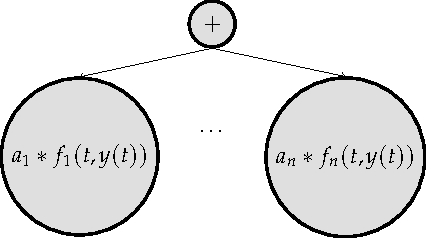
\includegraphics[width=0.5\textwidth]{"figures/doe_node_example.pdf"}
    \caption{Estructura del árbol de una ecuación diferencial lineal en los parámetros.}
    \label{tikzpicture:doe_node_example}
\end{figure}

Cada uno de los hijos del nodo que representa la parte derecha de una ecuación diferencial es un subárbol que representa la multiplicación de un parámetro con una función que no depende de parámetros.

Estos subárboles poseen como raíz un nodo con una operación de multiplicación y dos nodos hijos. El primero de ellos es un nodo hoja que representa el parámetro. El segundo hijo es un nodo que representa el subárbol computacional correspondiente a la función, utilizando la misma representación que plantea Koza \cite{zelinka2005analytic} pero con la peculiaridad de que sus hojas solo podrán almacenar variables, no parámetros. La figura \ref{tikzpicture:doe_term_node_example} muestra la estructura del subárbol que representa la multiplicación de un parámetro con una función que no depende de parámetros.

% \begin{center}
%     \begin{tikzpicture}[
%             roundnode/.style={circle, draw, fill=gray!25, very thick, minimum size=7mm},
%             squarednode/.style={rectangle, draw, fill=gray!25, very thick, minimum size=7mm}
%         ]
%         % Nodes
%         \node[roundnode]        (star)                            {$*$};
%         \node[squarednode]        (term_1)     [below left=of star]        {$a_i$};
%         \node[roundnode]        (term_n)     [below right=of star]        {$f_i(t, y(t))$};


%         %Lines
%         \draw [->] (star.south) -- (term_1.north);
%         \draw [->] (star.south) -- (term_n.north);
%     \end{tikzpicture}
% \end{center}

\begin{figure}[h]
    \centering
    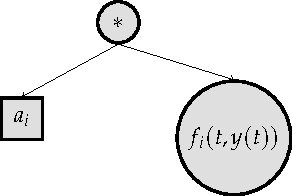
\includegraphics[width=0.5\textwidth]{"figures/doe_term_node_example.pdf"}
    \caption{Estructura del árbol de un término perteneciente a una ecuación diferencial lineal en los parámetros.}
    \label{tikzpicture:doe_term_node_example}
\end{figure}


Un sistema de ecuaciones diferenciales se puede representar como un árbol donde cada ecuación sea un hijo. Como ejemplo se puede utilizar el modelo poblacional SIR, que es lineal con respecto a sus parámetros, y su representación con la estructura propuesta sería la que se muestra en la figura \ref{tikzpicture:sir_example}.

% \begin{center}
%     \begin{tikzpicture}[
%             roundnode/.style={circle, draw, fill=gray!25, very thick, minimum size=7mm},
%             squarednode/.style={rectangle, draw, fill=gray!25, very thick, minimum size=5mm}
%         ]
%         % Nodes
%         \node[roundnode]        (system)                            {$SYSTEM$};

%         \node[roundnode]        (plus_S)     [below left=of system]        {$+$};
%         \node[roundnode]        (star_S_1)    [below left=of plus_S]    {$*$};
%         \node[squarednode]      (alpha_star_S_1)      [below left=of star_S_1]    {$a$};
%         \node[roundnode]        (neg_star_S_1)    [below=of star_S_1]    {$-$};
%         \node[roundnode]        (star_S_2)    [below=of neg_star_S_1]    {$*$};
%         \node[squarednode]      (S_star_S)       [below left=of star_S_2]   {$S$};
%         \node[squarednode]      (I_star_S)      [below=of star_S_2]   {$I$};

%         \node[roundnode]        (plus_I)     [below=of system]        {$+$};
%         \node[roundnode]        (star_I_1)    [below left=of plus_I]    {$*$};
%         \node[squarednode]      (alpha_star_I_1)      [below left=1cm and 0.5cm of star_I_1]    {$a$};
%         \node[roundnode]        (star_I_2)    [below=of star_I_1]    {$*$};
%         \node[squarednode]      (S_star_I)       [below left=1cm and 0.5cm of star_I_2]   {$S$};
%         \node[squarednode]      (I_star_I_1)      [below=of star_I_2]   {$I$};

%         \node[roundnode]        (star_I_3)    [below right=of plus_I]    {$*$};
%         \node[squarednode]      (beta_star_I_1)      [below=of star_I_3]    {$b$};
%         \node[roundnode]        (neg_star_I_1)    [below right=1cm and 0.5cm of star_I_3]    {$-$};
%         \node[squarednode]      (I_star_I_2)      [below=of neg_star_I_1]   {$I$};

%         \node[roundnode]        (plus_R)     [below right=of system]        {$+$};
%         \node[roundnode]        (star_R_1)    [below right=of plus_R]    {$*$};
%         \node[squarednode]      (beta_star_R_1)      [below=of star_R_1]    {$b$};
%         \node[squarednode]      (I_star_R)      [below right=of star_R_1]   {$I$};

%         %Lines
%         \draw [->] (system.south) -- (plus_S.north);
%         \draw[->] (system.south) -- (plus_I.north);
%         \draw[->] (system.south) -- (plus_R.north);

%         \draw[->] (plus_S.south) -- (star_S_1.north);
%         \draw[->] (star_S_1.south) -- (alpha_star_S_1.north);
%         \draw[->] (star_S_1.south) -- (neg_star_S_1.north);
%         \draw[->] (neg_star_S_1.south) -- (star_S_2.north);
%         \draw[->] (star_S_2.south) -- (S_star_S.north);
%         \draw[->] (star_S_2.south) -- (I_star_S.north);

%         \draw[->] (plus_I.south) -- (star_I_1.north);
%         \draw[->] (plus_I.south) -- (star_I_3.north);
%         \draw[->] (star_I_1.south) -- (alpha_star_I_1.north);
%         \draw[->] (star_I_1.south) -- (star_I_2.north);
%         \draw[->] (star_I_2.south) -- (S_star_I.north);
%         \draw[->] (star_I_2.south) -- (I_star_I_1.north);

%         \draw[->] (star_I_3.south) -- (beta_star_I_1.north);
%         \draw[->] (star_I_3.south) -- (neg_star_I_1.north);
%         \draw[->] (neg_star_I_1.south) -- (I_star_I_2.north);

%         \draw[->] (plus_R.south) -- (star_R_1.north);
%         \draw[->] (star_R_1.south) -- (beta_star_R_1.north);
%         \draw[->] (star_R_1.south) -- (I_star_R.north);
%     \end{tikzpicture}
% \end{center}

\begin{figure}[h]
    \centering
    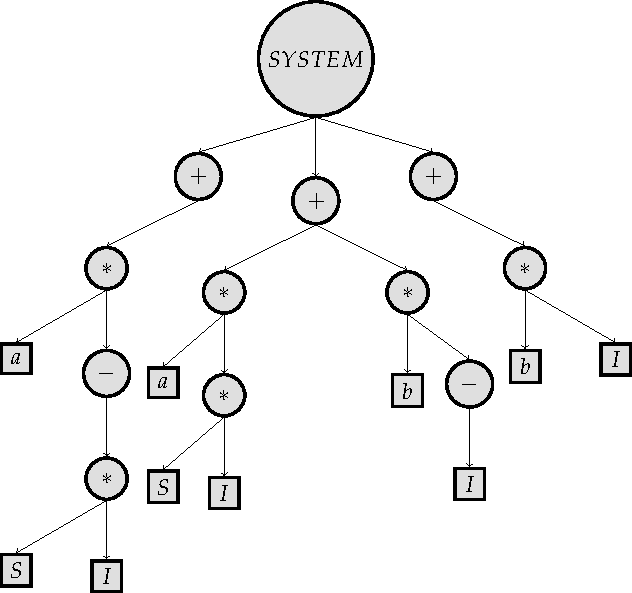
\includegraphics[width=0.5\textwidth]{"figures/sir_example.pdf"}
    \caption{Estructura del árbol que representa el modelo poblacional SIR.}
    \label{tikzpicture:sir_example}
\end{figure}

Con esta representación se pueden expresar todos los sistemas de ecuaciones diferenciales lineales en los parámetros en los que intervengan un conjunto de operaciones prefijadas de antemano, que son los posibles nodos interiores. Esta representación se utiliza para la representación de los modelos que se generan en el algoritmo de regresión simbólica que se detalla en la secciones \ref{section:mutation} y \ref{section:xcross}.

En un método de regresión simbólica es necesario tener una función de ajuste que permita conocer cuán cercanos son los datos predichos por el modelo con respecto a los datos observados. En la siguiente sección se propone un método para evaluar cuán cercanos se encuentran los datos predichos y observados.

\section{Determinar el costo de una solución}\label{section:solution_cost}

A partir de un conjunto de datos $M = \{(t_j, y_i(t_j)), i = 1, \dots, n, j = 1, \dots, m\}$ donde la función $y_i$ es desconocida, se puede aproximar el valor de las derivadas de $y_i$ en cada instante $t_j$ utilizando el método de diferencias finitas \cite{gaucel2014learning} en caso de que $M$ no posea ruido. Si el conjunto de datos $M$ tiene ruido se puede aproximar la función $y_i$ mediante un spline de suavizado cúbico. Con este spline de suavizado se puede obtener una aproximación del valor de la derivada de la función $y_i$ en cada instante $t_j$.

Luego de aproximar la derivada de las funciones $y_i$ en cada instante $t_j$ se puede generar un nuevo conjunto de la forma $\{(x_j, y'_{i_j}), x_j \in M, i = 1, \dots, n\}$ donde $y'_{i_j}$ es el valor de la aproximación de la derivada de la función $y_i$ en el instante $t_j$.

Por ejemplo, si se tienen el conjunto de datos sin ruido:

\begin{align*}
    \{ & (1, 1)     \\
       & (2, 4)     \\
       & (3, 9) \},
\end{align*}

y se desea conocer el valor aproximado de la derivada de la función $y$ en los instantes $1$ y $2$ se puede utilizar el método de diferencias finitas para obtener los datos:

\begin{align*}
    y'(1) & = \frac{y(2) - y(1)}{2 - 1} = 3  \\
    y'(2) & = \frac{y(3) - y(2)}{3 - 2} = 5.
\end{align*}

Con esta aproximación de la derivada se puede formar el nuevo conjunto de datos:

\begin{align*}
    \{ & ((1, 1), (3))    \\
       & ((2, 4), (5)) \}
\end{align*}

Se define el costo de un sistema de ecuaciones diferenciales $f$ para el conjunto de datos de la forma $\{(x_j, y'_j) \subset \mathbb{R}^{n+1} \times \mathbb{R}^n, j = 1, \dots, m\}$ como:

$$C = \frac{\sum_{i=1}^n\frac{\sum_{j=1}^{m}(y'_{i_j} - f_i(x_j))^2}{m}}{n},$$

donde:

$$f_i(x_j) = \sum_{k=1}^{p_i} a_{i_k} * g_{i_k}(x_j),$$

$f_1, f_2, \dots, f_n$ son las partes derechas de las ecuaciones del sistema y $p_i$ indica la cantidad de parámetros presentes en la ecuación $i$ del sistema. Mientras más pequeño es el valor del costo, mejor se describen los datos mediante el sistema $f$.

Al valor de $C$ se le agrega un factor de peso $P$, directamente proporcional a la cantidad de términos que posean las ecuaciones de la solución \cite{gplearnbloat}:

$$P = \begin{cases}
        Constant * node\_count(f), & \text{si } node\_count(f) \geq MAX\_NODES \\
        0,                         & \text{en otro caso}
    \end{cases}.$$

$Node\_count(f)$ es la cantidad de nodos presentes en la representación en forma de árbol computacional del sistema $f$. $Constant$ es una constante definida en la implementación y en los experimentos realizados en el capítulo \ref{chapter:results} se utiliza un valor de 9999.

El parámetro $MAX\_NODES$ se define junto con los demás parámetros del algoritmo genético y en los experimentos del capítulo \ref{chapter:results} se usaron valores entre 15 y 40. El factor de peso garantiza que si dos ecuaciones son capaces de generar los mismos puntos, la ecuación con menos términos tenga una mejor evaluación en la función objetivo.

Para que la suma $\sum_{j=1}^{m}(y'_{i_j} - f_i(x_j)) ^ 2$ sea la menor posible se debe minimizar la diferencia $(y'_{i_j} - f_i(x_j))^2$, y para ello que se crea, por cada ecuación del sistema, un sistema de ecuaciones de la forma $A_i * x_i = B_i$ donde:

\begin{align*}
    A_i & = \begin{pmatrix}
        g_{i_1}(x_1) & g_{i_2}(x_1) & \dots  & g_{i_k}(x_1) \\
        g_{i_1}(x_2) & g_{i_2}(x_2) &        & g_{i_k}(x_2) \\
        \vdots       & \vdots       & \ddots & \vdots       \\
        g_{i_1}(x_m) & g_{i_2}(x_m) &        & g_{i_k}(x_m)
    \end{pmatrix}
    \qquad
    x_i = \begin{bmatrix}
        a_{i_1} \\
        a_{i_2} \\
        \vdots  \\
        a_{i_k}
    \end{bmatrix}
    \qquad
    B_i = \begin{bmatrix}
        y'_{i_1} \\
        y'_{i_2} \\
        \vdots   \\
        y'_{i_m}
    \end{bmatrix}.
\end{align*}

El sistema $A_ix_i = B_i$ se resuelve usando la descomposición svd.

Por ejemplo, la segunda ecuación del modelo SIR es:

$$f_I (t,S,I,R) = a_{I_1} * g_{I_1}(t,S,I,R) + a_{I_2} * g_{I_2}(t,S,I,R),$$

donde:

$$g_{I_1}(t,S,I,R) = I*S$$

y

$$g_{I_2}(t,S,I,R) = -I.$$

Si se tiene el conjunto de datos de la forma $\{(x_j, y'_j) \subset \mathbb{R}^{4} \times \mathbb{R}^3, j = 1, \dots, 6\}$, donde $x_j$ representa los valores de $(t_j, S(t_j), I(t_j), R(T_j))$ y $y'_j$ representa los valores aproximados de $(S'(x_j), I'(x_j), R'(x_j))$:

\begin{align*}
    \{ ((1, 4, 9, 6) & ,  (0, 5, 0))     \\
    ((2, 6, 8, 2)    & ,  (0, 4, 0))     \\
    ((3, 3, 6, 8)    & ,  (0, 10, 0))    \\
    ((4, 5, 9, 8)    & ,  (0, 1, 0))     \\
    ((5, 6, 3, 10)   & , (0, 7, 0))      \\
    ((6, 8, 5, 7)    & ,  (0, 6, 0)) \},
\end{align*}

entonces se puede encontrar los valores de $a_1$ y $a_2$ que mejor ajusten los datos descritos formando el sistema de ecuaciones:

\begin{align*}
    A_I & = \begin{pmatrix}
        36 & -9 \\
        48 & -8 \\
        18 & -6 \\
        45 & -9 \\
        18 & -3 \\
        40 & -5
    \end{pmatrix}
    \qquad
    x_I = \begin{bmatrix}
        a_{I_1} \\
        a_{I_2}
    \end{bmatrix}
    \qquad
    B_I = \begin{bmatrix}
        5  \\
        4  \\
        10 \\
        1  \\
        7  \\
        6
    \end{bmatrix}.
\end{align*}

Al resolver el sistema de ecuaciones sobredeterminado se obtienen los parámetros $a_{I_1}$ = -0.03570806 y $a_{I_2}$ = -0.84347764. Este método se aplica para encontrar los parámetros de cada una de las ecuaciones del sistema y así se obtienen todos los parámetros del sistema.

Como se mencionó al inicio del capítulo, la propuesta de solución utiliza el método de regresión simbólica mediante el uso de un algoritmo genético para encontrar el sistema que mejor ajuste un conjunto de puntos. Para usar el algoritmo genético es necesario definir las operaciones de mutación, cruzamiento y selección. En la siguiente sección se describe la operación de mutación.

\section{Mutación}\label{section:mutation}

La operación de mutación genera un nuevo sistema de ecuaciones diferenciales a partir de otro existente. Esta operación selecciona el subárbol representante de una de las ecuaciones en el sistema y luego se realiza una de las siguientes modificaciones:

\begin{itemize}
    \item Eliminar un término (sumando de la ecuación) de la ecuación. Si se toman los sumandos de la ecuación como una lista de términos, el criterio consiste en seleccionar un término y eliminarlo.

          Por ejemplo, si se tiene la ecuación

          $$a_1 * y_1 + a_2 * -(y_1 * y_2),$$

          la lista de términos correspondientes sería:

          $$[a_1*y_1, a_2 * -(y_1 * y_2)].$$

          Si se selecciona eliminar el segundo término, la lista de términos correspondiente a la ecuación resultaría:

          $$[a_1 * y_1],$$

          y la ecuación resultante sería:

          $$a_1 * y_1.$$

          El ejemplo en forma de árbol computacional se muestra en la figura \ref{tikzpicture:mutation_delete_term}.

          \begin{center}
              %   \begin{adjustbox}{width=0.35\textwidth, keepaspectratio}
              %       \begin{tikzpicture}[
              %               roundnode_dashed/.style={circle, draw, dashed, fill=gray!25, very thick, minimum size=7mm},
              %               roundnode/.style={circle, draw, fill=gray!25, very thick, minimum size=7mm},
              %               squarednode/.style={rectangle, draw, fill=gray!25, very thick, minimum size=5mm},
              %           ]
              %           %Nodes
              %           \node[roundnode]      (plus)                             {$+$};
              %           \node[roundnode]           (star1)   [below left=of plus]    {$*$};
              %           \node[squarednode]         (a_1)   [below left=of star1]    {$a_1$};
              %           \node[squarednode]         (y_1)     [below=of star1]         {$y_1$};
              %           \node[roundnode_dashed]           (star2)   [below right=of plus]   {$*$};
              %           \node[squarednode]         (a_2)    [below left=of star2]    {$a_2$};
              %           \node[roundnode]           (neg)     [below=of star2]         {$-$};
              %           \node[roundnode]           (star3)   [below=of neg]         {$*$};
              %           \node[squarednode]         (y_1_2)   [below=of star3]   {$y_1$};
              %           \node[squarednode]         (y_2)     [below right=of star3]   {$y_2$};

              %           %Lines
              %           \draw[->] (plus.south) -- (star1.north);
              %           \draw[->] (plus.south) -- (star2.north);
              %           \draw[->] (star1.south) -- (a_1.north);
              %           \draw[->] (star1.south) -- (y_1.north);
              %           \draw[->] (star2.south) -- (a_2.north);
              %           \draw[->] (star2.south) -- (neg.north);
              %           \draw[->] (neg.south) -- (star3.north);
              %           \draw[->] (star3.south) -- (y_1_2.north);
              %           \draw[->] (star3.south) -- (y_2.north);
              %       \end{tikzpicture}%
              %   \end{adjustbox}

              %   \qquad

              %   \begin{adjustbox}{width=0.20\textwidth, keepaspectratio}
              %       \begin{tikzpicture}[
              %               roundnode_dashed/.style={circle, draw, dashed, fill=gray!25, very thick, minimum size=7mm},
              %               roundnode/.style={circle, draw, fill=gray!25, very thick, minimum size=7mm},
              %               squarednode/.style={rectangle, draw, fill=gray!25, very thick, minimum size=5mm},
              %           ]
              %           %Nodes
              %           \node[roundnode]      (plus)                             {$+$};
              %           \node[roundnode]           (star1)   [below =of plus]    {$*$};
              %           \node[squarednode]         (a_1)   [below left=of star1]    {$a_1$};
              %           \node[squarednode]         (y_1)     [below right=of star1]         {$y_1$};

              %           %Lines
              %           \draw[->] (plus.south) -- (star1.north);
              %           \draw[->] (star1.south) -- (a_1.north);
              %           \draw[->] (star1.south) -- (y_1.north);
              %       \end{tikzpicture}%
              %   \end{adjustbox}

              \begin{figure}[h]
                  \centering
                  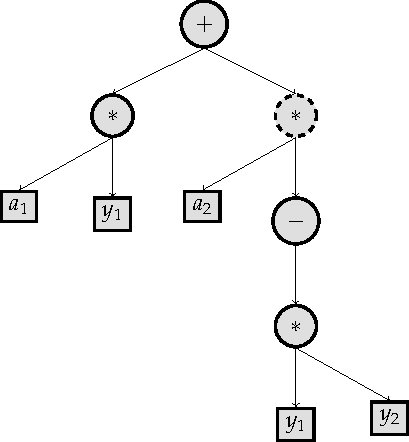
\includegraphics[width=0.3\textwidth]{"figures/mutation_delete_term_1.pdf"}
                  \qquad
                  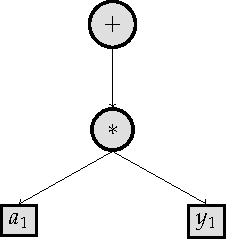
\includegraphics[width=0.3\textwidth]{"figures/mutation_delete_term_2.pdf"}
                  \caption{Ejemplo de mutación mediante la eliminación de un término en una ecuación.}
                  \label{tikzpicture:mutation_delete_term}
              \end{figure}
          \end{center}

    \item Añadir un término a la ecuación. Si se toman los sumandos de la ecuación como una lista de términos, el criterio consiste en crear un término y añadirlo.

          Por ejemplo, si se tiene la ecuación

          $$a_1 * y_1,$$

          la lista de términos correspondientes sería:

          $$[a_1*y_1].$$

          Si se selecciona añadir como segundo sumando el término $a_2 * y_2$, la lista de términos correspondiente a la ecuación resultaría:

          $$[a_1*y_1, a_2 * y_2],$$

          y la ecuación resultante sería:

          $$a_1 * y_1 + a_2 * y_2.$$

          El ejemplo en forma de árbol computacional se muestra en la figura \ref{tikzpicture:mutation_add_term}.

          \begin{center}
              %   \begin{adjustbox}{width=0.25\textwidth, keepaspectratio}
              %       \begin{tikzpicture}[
              %               roundnode_dashed/.style={circle, draw, dashed, fill=gray!25, very thick, minimum size=7mm},
              %               roundnode/.style={circle, draw, fill=gray!25, very thick, minimum size=7mm},
              %               squarednode/.style={rectangle, draw, fill=gray!25, very thick, minimum size=5mm},
              %           ]
              %           %Nodes
              %           \node[roundnode]      (plus)                             {$+$};
              %           \node[roundnode]           (star1)   [below =of plus]    {$*$};
              %           \node[squarednode]         (a_1)   [below left=of star1]    {$a_1$};
              %           \node[squarednode]         (y_1)     [below right=of star1]         {$y_1$};

              %           %Lines
              %           \draw[->] (plus.south) -- (star1.north);
              %           \draw[->] (star1.south) -- (a_1.north);
              %           \draw[->] (star1.south) -- (y_1.north);
              %       \end{tikzpicture}%
              %   \end{adjustbox}
              %   \qquad
              %   \begin{adjustbox}{width=0.35\textwidth, keepaspectratio}
              %       \begin{tikzpicture}[
              %               roundnode_dashed/.style={circle, draw, dashed, fill=gray!25, very thick, minimum size=7mm},
              %               roundnode/.style={circle, draw, fill=gray!25, very thick, minimum size=7mm},
              %               squarednode/.style={rectangle, draw, fill=gray!25, very thick, minimum size=5mm},
              %           ]
              %           %Nodes
              %           \node[roundnode]      (plus)                             {$+$};
              %           \node[roundnode]           (star1)   [below left=of plus]    {$*$};
              %           \node[squarednode]         (a_1)   [below left=of star1]    {$a_1$};
              %           \node[squarednode]         (y_1)     [below=of star1]         {$y_1$};
              %           \node[roundnode_dashed]           (star2)   [below right=of plus]   {$*$};
              %           \node[squarednode]         (a_2)    [below=of star2]    {$a_2$};
              %           \node[squarednode]           (y_2)     [below right=of star2]         {$y_2$};

              %           %Lines
              %           \draw[->] (plus.south) -- (star1.north);
              %           \draw[->] (plus.south) -- (star2.north);
              %           \draw[->] (star1.south) -- (a_1.north);
              %           \draw[->] (star1.south) -- (y_1.north);
              %           \draw[->] (star2.south) -- (a_2.north);
              %           \draw[->] (star2.south) -- (y_2.north);
              %       \end{tikzpicture}%
              %   \end{adjustbox}

              \begin{figure}[H]
                  \centering
                  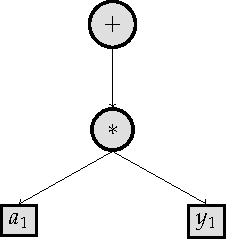
\includegraphics[width=0.3\textwidth]{"figures/mutation_add_term_1.pdf"}
                  \qquad
                  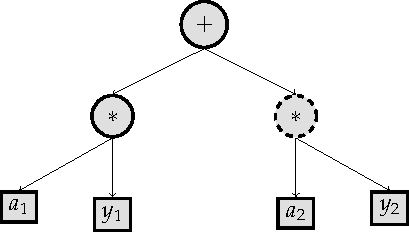
\includegraphics[width=0.5\textwidth]{"figures/mutation_add_term_2.pdf"}
                  \caption{Ejemplo de mutación mediante la adición de un término a una ecuación.}
                  \label{tikzpicture:mutation_add_term}
              \end{figure}
          \end{center}

    \item Mutar un término de la ecuación. Si se toman los sumandos de la ecuación como una lista de términos, el criterio consiste en seleccionar un término y dentro de su representación en forma de árbol computacional, tomar un nodo y aplicarle una de las siguientes modificaciones.
          Si el nodo representa una operación:

          \begin{itemize}
              \item Se cambia la operación en el nodo por uno que posea la misma cantidad de argumentos del operador:

                    Por ejempo, si se tiene el término $y_1 + (y_2 - y_3)$ se puede sustituir la resta por una suma resultando $y_1 + (y_2 + y_3)$. Se muestra en forma de árbol computacional en la figura \ref{tikzpicture:mutation_change_operation}.

                    \begin{center}
                        %   \begin{adjustbox}{width=0.25\textwidth, keepaspectratio}
                        %       \begin{tikzpicture}[
                        %               roundnode_dashed/.style={circle, draw, dashed, fill=gray!25, very thick, minimum size=7mm},
                        %               roundnode/.style={circle, draw, fill=gray!25, very thick, minimum size=7mm},
                        %               squarednode/.style={rectangle, draw, fill=gray!25, very thick, minimum size=5mm},
                        %           ]
                        %           %               %Nodes
                        %           \node[roundnode]      (plus)                            {$+$};
                        %           \node[squarednode]    (y_1)     [below left=of plus]    {$y_1$};
                        %           \node[roundnode_dashed]      (sub)     [below right=of plus]   {$-$};
                        %           \node[squarednode]    (y_2)     [below left=of sub]     {$y_2$};
                        %           \node[squarednode]    (y_3)     [below right=of sub]    {$y_3$};


                        %           %   %Lines
                        %           \draw[->] (plus.south) -- (y_1.north);
                        %           \draw[->] (plus.south) -- (sub.north);
                        %           \draw[->] (sub.south) -- (y_2.north);
                        %           \draw[->] (sub.south) -- (y_3.north);
                        %       \end{tikzpicture}%
                        %   \end{adjustbox}
                        %   \qquad
                        %   \begin{adjustbox}{width=0.25\textwidth, keepaspectratio}
                        %       \begin{tikzpicture}[
                        %               roundnode_dashed/.style={circle, draw, dashed, fill=gray!25, very thick, minimum size=7mm},
                        %               roundnode/.style={circle, draw, fill=gray!25, very thick, minimum size=7mm},
                        %               squarednode/.style={rectangle, draw, fill=gray!25, very thick, minimum size=5mm},
                        %           ]
                        %           %Nodes
                        %           \node[roundnode]      (plus)                            {$+$};
                        %           \node[squarednode]    (y_1)     [below left=of plus]    {$y_1$};
                        %           \node[roundnode_dashed]      (plus_2)     [below right=of plus]   {$+$};
                        %           \node[squarednode]    (y_2)     [below left=of plus_2]     {$y_2$};
                        %           \node[squarednode]    (y_3)     [below right=of plus_2]    {$y_3$};


                        %           %   %Lines
                        %           \draw[->] (plus.south) -- (y_1.north);
                        %           \draw[->] (plus.south) -- (plus_2.north);
                        %           \draw[->] (plus_2.south) -- (y_2.north);
                        %           \draw[->] (plus_2.south) -- (y_3.north);
                        %       \end{tikzpicture}%
                        %   \end{adjustbox}
                        \begin{figure}[h]
                            \centering
                            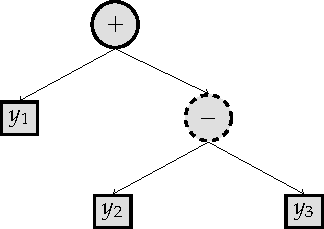
\includegraphics[width=0.3\textwidth]{"figures/mutation_change_operation_1.pdf"}
                            \qquad
                            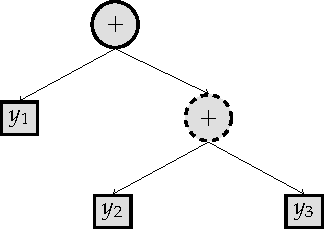
\includegraphics[width=0.3\textwidth]{"figures/mutation_change_operation_2.pdf"}
                            \caption{Ejemplo de mutación mediante la modificación de una operación en un término.}
                            \label{tikzpicture:mutation_change_operation}
                        \end{figure}
                    \end{center}

              \item Se elimina el nodo, colocando en su lugar su primer hijo.

                    Por ejempo, si se tiene el término $y_1 + (y_2 - y_3)$ se puede sustituir la resta por su primer argumento obteniéndose $y_1 + y_2$. Se muestra en forma de árbol computacional en la figura \ref{tikzpicture:mutation_delete_operation}.

                    \begin{center}
                        %   \begin{adjustbox}{width=0.25\textwidth, keepaspectratio}
                        %       \begin{tikzpicture}[
                        %               roundnode_dashed/.style={circle, draw, dashed, fill=gray!25, very thick, minimum size=7mm},
                        %               roundnode/.style={circle, draw, fill=gray!25, very thick, minimum size=7mm},
                        %               squarednode/.style={rectangle, draw, fill=gray!25, very thick, minimum size=5mm},
                        %           ]
                        %           %Nodes
                        %           \node[roundnode]      (plus)                            {$+$};
                        %           \node[squarednode]    (y_1)     [below left=of plus]    {$y_1$};
                        %           \node[roundnode_dashed]      (sub)     [below right=of plus]   {$-$};
                        %           \node[squarednode]    (y_2)     [below left=of sub]     {$y_2$};
                        %           \node[squarednode]    (y_3)     [below right=of sub]    {$y_3$};


                        %           %   %Lines
                        %           \draw[->] (plus.south) -- (y_1.north);
                        %           \draw[->] (plus.south) -- (sub.north);
                        %           \draw[->] (sub.south) -- (y_2.north);
                        %           \draw[->] (sub.south) -- (y_3.north);
                        %       \end{tikzpicture}%
                        %   \end{adjustbox}
                        %   \qquad
                        %   \begin{adjustbox}{width=0.25\textwidth, keepaspectratio}
                        %       \begin{tikzpicture}[
                        %               roundnode_dashed/.style={circle, draw, dashed, fill=gray!25, very thick, minimum size=7mm},
                        %               roundnode/.style={circle, draw, fill=gray!25, very thick, minimum size=7mm},
                        %               squarednode/.style={rectangle, draw, fill=gray!25, very thick, minimum size=5mm},
                        %           ]
                        %           %Nodes
                        %           \node[roundnode]      (plus)                            {$+$};
                        %           \node[squarednode]    (y_1)     [below left=of plus]    {$y_1$};
                        %           \node[squarednode]    (y_2)     [below right=of plus]     {$y_2$};


                        %           %   %Lines
                        %           \draw[->] (plus.south) -- (y_1.north);
                        %           \draw[->] (plus.south) -- (y_2.north);
                        %       \end{tikzpicture}%
                        %   \end{adjustbox}
                        \begin{figure}[h]
                            \centering
                            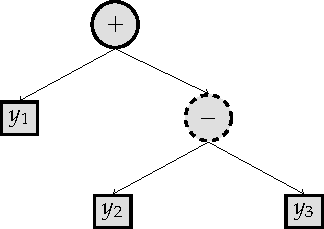
\includegraphics[width=0.3\textwidth]{"figures/mutation_delete_operation_1.pdf"}
                            \qquad
                            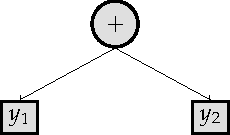
\includegraphics[width=0.3\textwidth]{"figures/mutation_delete_operation_2.pdf"}
                            \caption{Ejemplo de mutación mediante la eliminación de una operación en un término.}
                            \label{tikzpicture:mutation_delete_operation}
                        \end{figure}
                    \end{center}

              \item Se cambia el nodo por uno nuevo que represente una operación aleatoria colocando como hijos nuevos árboles de expresiones aleatorias y como último hijo el nodo original que se seleccionó.

                    Por ejempo, si se tiene el término $y_1 + (y_2 - y_3)$ se puede sustituir la resta por una multiplicación colocando como segundo factor la misma resta obteniéndose $y_1 + y_4 * (y_2 - y_3)$. Se expresa en forma de árbol computacional en la figura \ref{tikzpicture:mutation_add_operation}.

                    \begin{center}
                        %   \begin{adjustbox}{width=0.25\textwidth, keepaspectratio}
                        %       \begin{tikzpicture}[
                        %               roundnode_dashed/.style={circle, draw, dashed, fill=gray!25, very thick, minimum size=7mm},
                        %               roundnode/.style={circle, draw, fill=gray!25, very thick, minimum size=7mm},
                        %               squarednode/.style={rectangle, draw, fill=gray!25, very thick, minimum size=5mm},
                        %           ]
                        %           %Nodes
                        %           \node[roundnode]      (plus)                            {$+$};
                        %           \node[squarednode]    (y_1)     [below left=of plus]    {$y_1$};
                        %           \node[roundnode_dashed]      (sub)     [below right=of plus]   {$-$};
                        %           \node[squarednode]    (y_2)     [below left=of sub]     {$y_2$};
                        %           \node[squarednode]    (y_3)     [below right=of sub]    {$y_3$};


                        %           %   %Lines
                        %           \draw[->] (plus.south) -- (y_1.north);
                        %           \draw[->] (plus.south) -- (sub.north);
                        %           \draw[->] (sub.south) -- (y_2.north);
                        %           \draw[->] (sub.south) -- (y_3.north);
                        %       \end{tikzpicture}%
                        %   \end{adjustbox}
                        %   \qquad
                        %   \begin{adjustbox}{width=0.25\textwidth, keepaspectratio}
                        %       \begin{tikzpicture}[
                        %               roundnode_dashed/.style={circle, draw, dashed, fill=gray!25, very thick, minimum size=7mm},
                        %               roundnode/.style={circle, draw, fill=gray!25, very thick, minimum size=7mm},
                        %               squarednode/.style={rectangle, draw, fill=gray!25, very thick, minimum size=5mm},
                        %           ]
                        %           %Nodes
                        %           \node[roundnode]      (plus)                            {$+$};
                        %           \node[squarednode]    (y_1)     [below left=of plus]    {$y_1$};
                        %           \node[roundnode]    (star)  [below right=of plus]   {$*$};
                        %           \node[squarednode]  (y_4)   [below left=of star]        {$y_4$};
                        %           \node[roundnode_dashed]      (sub)     [below right=of star]   {$-$};
                        %           \node[squarednode]    (y_2)     [below left=of sub]     {$y_2$};
                        %           \node[squarednode]    (y_3)     [below right=of sub]    {$y_3$};


                        %           %   %Lines
                        %           \draw[->] (plus.south) -- (y_1.north);
                        %           \draw[->] (plus.south) -- (star.north);
                        %           \draw[->] (star.south) -- (y_4.north);
                        %           \draw[->] (star.south) -- (sub.north);
                        %           \draw[->] (sub.south) -- (y_2.north);
                        %           \draw[->] (sub.south) -- (y_3.north);
                        %       \end{tikzpicture}%
                        %   \end{adjustbox}
                        \begin{figure}[h]
                            \centering
                            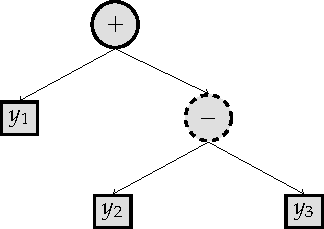
\includegraphics[width=0.4\textwidth]{"figures/mutation_add_operation_1.pdf"}
                            \qquad
                            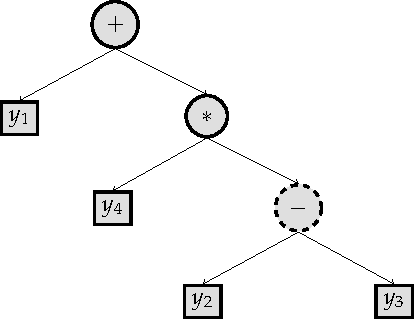
\includegraphics[width=0.4\textwidth]{"figures/mutation_add_operation_2.pdf"}
                            \caption{Ejemplo de mutación mediante la adición de un nuevo nodo a un término.}
                            \label{tikzpicture:mutation_add_operation}
                        \end{figure}
                    \end{center}

          \end{itemize}

          Si el nodo representa una variable:

          \begin{itemize}
              \item Cambiar la variable por otra permitida dentro de la ecuación.

                    Por ejempo, si se tiene el término $y_1 + (y_2 - y_3)$ se puede sustituir la variable $y_3$ obteniéndose $y_1 + (y_2 - y_1)$. Se plantea en forma de árbol computacional en la figura \ref{tikzpicture:mutation_change_variable}.

                    \begin{center}
                        %   \begin{adjustbox}{width=0.25\textwidth, keepaspectratio}
                        %       \begin{tikzpicture}[
                        %               roundnode/.style={circle, draw, fill=gray!25, very thick, minimum size=7mm},
                        %               squarednode/.style={rectangle, draw, fill=gray!25, very thick, minimum size=5mm},
                        %               squarednode_dashed/.style={rectangle, draw, dashed, fill=gray!25, very thick, minimum size=7mm},
                        %           ]
                        %           %Nodes
                        %           \node[roundnode]      (plus)                            {$+$};
                        %           \node[squarednode]    (y_1)     [below left=of plus]    {$y_1$};
                        %           \node[roundnode]      (sub)     [below right=of plus]   {$-$};
                        %           \node[squarednode]    (y_2)     [below left=of sub]     {$y_2$};
                        %           \node[squarednode_dashed]    (y_3)     [below right=of sub]    {$y_3$};


                        %           %   %Lines
                        %           \draw[->] (plus.south) -- (y_1.north);
                        %           \draw[->] (plus.south) -- (sub.north);
                        %           \draw[->] (sub.south) -- (y_2.north);
                        %           \draw[->] (sub.south) -- (y_3.north);
                        %       \end{tikzpicture}%
                        %   \end{adjustbox}
                        %   \qquad
                        %   \begin{adjustbox}{width=0.25\textwidth, keepaspectratio}
                        %       \begin{tikzpicture}[
                        %               roundnode/.style={circle, draw, fill=gray!25, very thick, minimum size=7mm},
                        %               squarednode/.style={rectangle, draw, fill=gray!25, very thick, minimum size=5mm},
                        %               squarednode_dashed/.style={rectangle, draw, dashed, fill=gray!25, very thick, minimum size=7mm},
                        %           ]
                        %           %Nodes
                        %           \node[roundnode]      (plus)                            {$+$};
                        %           \node[squarednode]    (y_1)     [below left=of plus]    {$y_1$};
                        %           \node[roundnode]      (sub)     [below right=of plus]   {$-$};
                        %           \node[squarednode]    (y_2)     [below left=of sub]     {$y_2$};
                        %           \node[squarednode_dashed]    (y_1_2)     [below right=of sub]    {$y_1$};


                        %           %   %Lines
                        %           \draw[->] (plus.south) -- (y_1.north);
                        %           \draw[->] (plus.south) -- (sub.north);
                        %           \draw[->] (sub.south) -- (y_2.north);
                        %           \draw[->] (sub.south) -- (y_1_2.north);
                        %       \end{tikzpicture}%
                        %   \end{adjustbox}
                        \begin{figure}[!h]
                            \centering
                            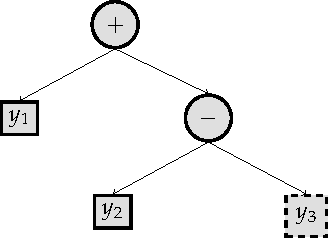
\includegraphics[width=0.3\textwidth]{"figures/mutation_change_variable_1.pdf"}
                            \qquad
                            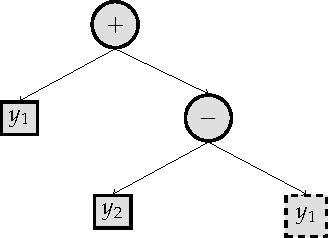
\includegraphics[width=0.3\textwidth]{"figures/mutation_change_variable_2.pdf"}
                            \caption{Ejemplo de mutación mediante la modificación de una variable un término.}
                            \label{tikzpicture:mutation_change_variable}
                        \end{figure}
                    \end{center}

              \item Cambiar la variable por un nodo que represente una operación aleatoria donde el primer hijo es la variable seleccionada y el resto de hijos son nuevos árboles de expresiones aleatorias.

                    Por ejempo, si se tiene el término $y_1 + (y_2 - y_3)$ se puede sustituir la variable $y_3$ por una multiplicación donde el primer factor sea la misma variable $y_3$ y el segundo factor sea la variable $y_2$, obteniéndose $y_1 + (y_2 - y_3 * y_2)$. Se expresa en forma de árbol computacional en la figura \ref{tikzpicture:mutation_change_variable_by_node}.

                    \begin{center}
                        %   \begin{adjustbox}{width=0.25\textwidth, keepaspectratio}
                        %       \begin{tikzpicture}[
                        %               roundnode/.style={circle, draw, fill=gray!25, very thick, minimum size=7mm},
                        %               squarednode/.style={rectangle, draw, fill=gray!25, very thick, minimum size=5mm},
                        %               squarednode_dashed/.style={rectangle, draw, dashed, fill=gray!25, very thick, minimum size=7mm},
                        %           ]
                        %           %Nodes
                        %           \node[roundnode]      (plus)                            {$+$};
                        %           \node[squarednode]    (y_1)     [below left=of plus]    {$y_1$};
                        %           \node[roundnode]      (sub)     [below right=of plus]   {$-$};
                        %           \node[squarednode]    (y_2)     [below left=of sub]     {$y_2$};
                        %           \node[squarednode_dashed]    (y_3)     [below right=of sub]    {$y_3$};


                        %           %   %Lines
                        %           \draw[->] (plus.south) -- (y_1.north);
                        %           \draw[->] (plus.south) -- (sub.north);
                        %           \draw[->] (sub.south) -- (y_2.north);
                        %           \draw[->] (sub.south) -- (y_3.north);
                        %       \end{tikzpicture}%
                        %   \end{adjustbox}
                        %   \qquad
                        %   \begin{adjustbox}{width=0.25\textwidth, keepaspectratio}
                        %       \begin{tikzpicture}[
                        %               roundnode/.style={circle, draw, fill=gray!25, very thick, minimum size=7mm},
                        %               squarednode/.style={rectangle, draw, fill=gray!25, very thick, minimum size=5mm},
                        %               squarednode_dashed/.style={rectangle, draw, dashed, fill=gray!25, very thick, minimum size=7mm},
                        %           ]
                        %           %Nodes
                        %           \node[roundnode]      (plus)                            {$+$};
                        %           \node[squarednode]    (y_1)     [below left=of plus]    {$y_1$};
                        %           \node[roundnode]    (sub)  [below right=of plus]   {$-$};
                        %           \node[squarednode]  (y_2)   [below left=of sub]        {$y_2$};
                        %           \node[roundnode]      (star)     [below right=of sub]   {$*$};
                        %           \node[squarednode_dashed]    (y_3)     [below left=of star]    {$y_3$};
                        %           \node[squarednode]    (y_2_2)     [below right=of star]     {$y_2$};


                        %           %   %Lines
                        %           \draw[->] (plus.south) -- (y_1.north);
                        %           \draw[->] (plus.south) -- (sub.north);
                        %           \draw[->] (sub.south) -- (y_2.north);
                        %           \draw[->] (sub.south) -- (star.north);
                        %           \draw[->] (star.south) -- (y_3.north);
                        %           \draw[->] (star.south) -- (y_2_2.north);
                        %       \end{tikzpicture}%
                        %   \end{adjustbox}
                        \begin{figure}[h]
                            \centering
                            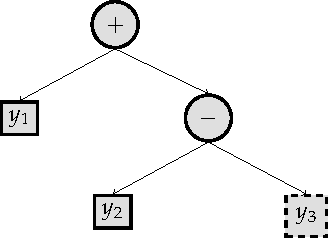
\includegraphics[width=0.4\textwidth]{"figures/mutation_change_variable_by_node_1.pdf"}
                            \qquad
                            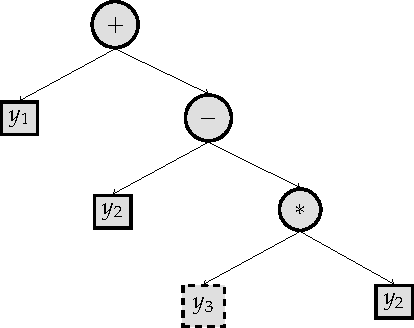
\includegraphics[width=0.4\textwidth]{"figures/mutation_change_variable_by_node_2.pdf"}
                            \caption{Ejemplo de mutación mediante la modificación de un nodo representante de una variable por una operación en un término.}
                            \label{tikzpicture:mutation_change_variable_by_node}
                        \end{figure}
                    \end{center}
          \end{itemize}
\end{itemize}

Como ejemplo de una operación de mutación se puede tomar el sistema:

\begin{align*}
    S' & = - a_1 * S * I         \\
    I' & = a_2 * S * I - a_3 * I \\
    R' & = a_4 * I,
\end{align*}

y se puede realizar la mutación de eliminar el segundo término de la segunda ecuación quedando como resultado el sistema

\begin{align*}
    S' & = - a_1 * S * I \\
    I' & = a_2 * S * I   \\
    R' & = a_4 * I,
\end{align*}

Este ejemplo se representa en forma de árbol computacional en la figura \ref{tikzpicture:mutation_sir}:

\begin{center}
    % \begin{adjustbox}{width=0.5\textwidth, keepaspectratio}
    %     \begin{tikzpicture}[
    %             roundnode/.style={circle, draw, fill=gray!25, very thick, minimum size=7mm},
    %             squarednode/.style={rectangle, draw, fill=gray!25, very thick, minimum size=5mm},
    %             roundnode_dashed/.style={circle, draw, dashed, fill=gray!25, very thick, minimum size=7mm},
    %         ]
    %         % Nodes
    %         \node[roundnode]        (system)                            {$SYSTEM$};

    %         \node[roundnode]        (plus_S)     [below left=of system]        {$+$};
    %         \node[roundnode]        (star_S_1)    [below left=of plus_S]    {$*$};
    %         \node[squarednode]      (alpha_star_S_1)      [below left=of star_S_1]    {$a_1$};
    %         \node[roundnode]        (neg_star_S_1)    [below=of star_S_1]    {$-$};
    %         \node[roundnode]        (star_S_2)    [below=of neg_star_S_1]    {$*$};
    %         \node[squarednode]      (S_star_S)       [below left=of star_S_2]   {$S$};
    %         \node[squarednode]      (I_star_S)      [below=of star_S_2]   {$I$};

    %         \node[roundnode]        (plus_I)     [below=of system]        {$+$};
    %         \node[roundnode]        (star_I_1)    [below left=of plus_I]    {$*$};
    %         \node[squarednode]      (alpha_star_I_1)      [below left=1cm and 0.5cm of star_I_1]    {$a_2$};
    %         \node[roundnode]        (star_I_2)    [below=of star_I_1]    {$*$};
    %         \node[squarednode]      (S_star_I)       [below left=1cm and 0.5cm of star_I_2]   {$S$};
    %         \node[squarednode]      (I_star_I_1)      [below=of star_I_2]   {$I$};

    %         \node[roundnode_dashed]        (star_I_3)    [below right=of plus_I]    {$*$};
    %         \node[squarednode]      (beta_star_I_1)      [below=of star_I_3]    {$a_3$};
    %         \node[roundnode]        (neg_star_I_1)    [below right=1cm and 0.5cm of star_I_3]    {$-$};
    %         \node[squarednode]      (I_star_I_2)      [below=of neg_star_I_1]   {$I$};

    %         \node[roundnode]        (plus_R)     [below right=of system]        {$+$};
    %         \node[roundnode]        (star_R_1)    [below right=of plus_R]    {$*$};
    %         \node[squarednode]      (beta_star_R_1)      [below=of star_R_1]    {$a_4$};
    %         \node[squarednode]      (I_star_R)      [below right=of star_R_1]   {$I$};

    %         %Lines
    %         \draw [->] (system.south) -- (plus_S.north);
    %         \draw[->] (system.south) -- (plus_I.north);
    %         \draw[->] (system.south) -- (plus_R.north);

    %         \draw[->] (plus_S.south) -- (star_S_1.north);
    %         \draw[->] (star_S_1.south) -- (alpha_star_S_1.north);
    %         \draw[->] (star_S_1.south) -- (neg_star_S_1.north);
    %         \draw[->] (neg_star_S_1.south) -- (star_S_2.north);
    %         \draw[->] (star_S_2.south) -- (S_star_S.north);
    %         \draw[->] (star_S_2.south) -- (I_star_S.north);

    %         \draw[->] (plus_I.south) -- (star_I_1.north);
    %         \draw[->] (plus_I.south) -- (star_I_3.north);
    %         \draw[->] (star_I_1.south) -- (alpha_star_I_1.north);
    %         \draw[->] (star_I_1.south) -- (star_I_2.north);
    %         \draw[->] (star_I_2.south) -- (S_star_I.north);
    %         \draw[->] (star_I_2.south) -- (I_star_I_1.north);

    %         \draw[->] (star_I_3.south) -- (beta_star_I_1.north);
    %         \draw[->] (star_I_3.south) -- (neg_star_I_1.north);
    %         \draw[->] (neg_star_I_1.south) -- (I_star_I_2.north);

    %         \draw[->] (plus_R.south) -- (star_R_1.north);
    %         \draw[->] (star_R_1.south) -- (beta_star_R_1.north);
    %         \draw[->] (star_R_1.south) -- (I_star_R.north);
    %     \end{tikzpicture}
    % \end{adjustbox}

    \begin{figure}[h]
        \centering
        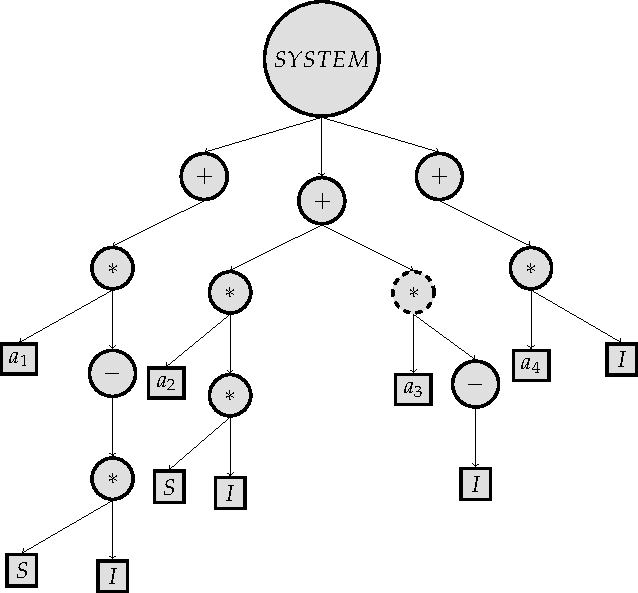
\includegraphics[width=0.6\textwidth]{"figures/mutation_sir_1.pdf"}
        \qquad
        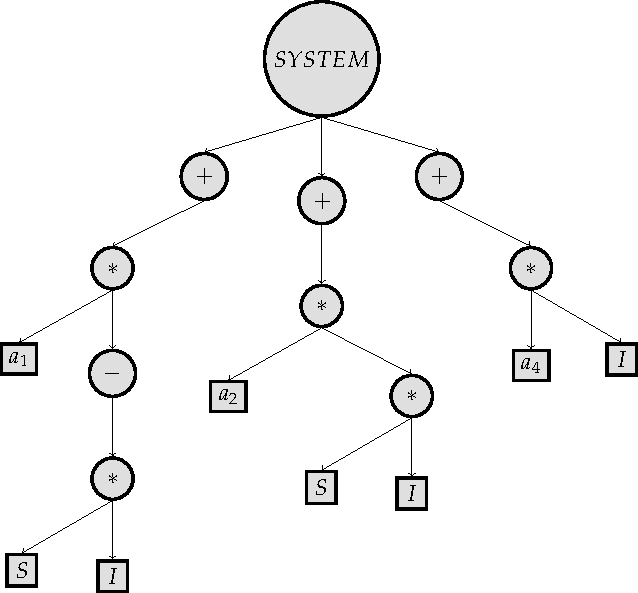
\includegraphics[width=0.6\textwidth]{"figures/mutation_sir_2.pdf"}
        \caption{Ejemplo de mutación mediante la eliminación de un término en una ecuación.}
        \label{tikzpicture:mutation_sir}
    \end{figure}

\end{center}

% \begin{center}
%     \begin{adjustbox}{width=0.5\textwidth, keepaspectratio}
%         \begin{tikzpicture}[
%                 roundnode/.style={circle, draw, fill=gray!25, very thick, minimum size=7mm},
%                 squarednode/.style={rectangle, draw, fill=gray!25, very thick, minimum size=5mm},
%                 roundnode_dashed/.style={circle, draw, dashed, fill=gray!25, very thick, minimum size=7mm},
%             ]
%             % Nodes
%             \node[roundnode]        (system)                            {$SYSTEM$};

%             \node[roundnode]        (plus_S)     [below left=of system]        {$+$};
%             \node[roundnode]        (star_S_1)    [below left=of plus_S]    {$*$};
%             \node[squarednode]      (alpha_star_S_1)      [below left=of star_S_1]    {$a_1$};
%             \node[roundnode]        (neg_star_S_1)    [below=of star_S_1]    {$-$};
%             \node[roundnode]        (star_S_2)    [below=of neg_star_S_1]    {$*$};
%             \node[squarednode]      (S_star_S)       [below left=of star_S_2]   {$S$};
%             \node[squarednode]      (I_star_S)      [below=of star_S_2]   {$I$};

%             \node[roundnode]        (plus_I)     [below=of system]        {$+$};
%             \node[roundnode]        (star_I_1)    [below=of plus_I]    {$*$};
%             \node[squarednode]      (alpha_star_I_1)      [below left=of star_I_1]    {$a_2$};
%             \node[roundnode]        (star_I_2)    [below right=of star_I_1]    {$*$};
%             \node[squarednode]      (S_star_I)       [below left=of star_I_2]   {$S$};
%             \node[squarednode]      (I_star_I_1)      [below=of star_I_2]   {$I$};

%             \node[roundnode]        (plus_R)     [below right=of system]        {$+$};
%             \node[roundnode]        (star_R_1)    [below right=of plus_R]    {$*$};
%             \node[squarednode]      (beta_star_R_1)      [below=of star_R_1]    {$a_4$};
%             \node[squarednode]      (I_star_R)      [below right=of star_R_1]   {$I$};

%             %Lines
%             \draw [->] (system.south) -- (plus_S.north);
%             \draw[->] (system.south) -- (plus_I.north);
%             \draw[->] (system.south) -- (plus_R.north);

%             \draw[->] (plus_S.south) -- (star_S_1.north);
%             \draw[->] (star_S_1.south) -- (alpha_star_S_1.north);
%             \draw[->] (star_S_1.south) -- (neg_star_S_1.north);
%             \draw[->] (neg_star_S_1.south) -- (star_S_2.north);
%             \draw[->] (star_S_2.south) -- (S_star_S.north);
%             \draw[->] (star_S_2.south) -- (I_star_S.north);

%             \draw[->] (plus_I.south) -- (star_I_1.north);
%             \draw[->] (star_I_1.south) -- (alpha_star_I_1.north);
%             \draw[->] (star_I_1.south) -- (star_I_2.north);
%             \draw[->] (star_I_2.south) -- (S_star_I.north);
%             \draw[->] (star_I_2.south) -- (I_star_I_1.north);

%             \draw[->] (plus_R.south) -- (star_R_1.north);
%             \draw[->] (star_R_1.south) -- (beta_star_R_1.north);
%             \draw[->] (star_R_1.south) -- (I_star_R.north);
%         \end{tikzpicture}
%     \end{adjustbox}
% \end{center}

Con estas modificaciones que se le pueden realizar a un sistema de ecuaciones diferenciales lineales en los parámetros se define la operación de mutación que se utiliza en el algoritmo genético que se emplea en este trabajo. Otra de las operaciones que se deben definir con el fin de implementar un algoritmo genético es el cruzamiento, que se describe en la siguiente sección.

\section{Cruzamiento}\label{section:xcross}

En la operación de cruzamiento se obtiene un nuevo sistema de ecuaciones diferenciales combinando propiedades de dos sistemas existentes A y B. Esta operación selecciona un nodo aleatorio dentro del árbol A que no represente un parámtro y un nodo dentro del árbol B que tampoco represente un parámetro, siguiendo un conjunto de reglas. Una vez escogidos los nodos se remplaza el subárbol del nodo seleccionado en A por el subárbol del nodo seleccionado en B, resultando en A un nuevo sistema de ecuaciones diferenciales.

En dependencia del nodo seleccionado en A se escoge el nodo en B siguiendo las siguientes reglas:


\begin{itemize}
    \item Si el nodo seleccionado en A es el representante de la i-ésima ecuación en el sistema, se escoge el nodo representante de la i-ésima ecuación en el sistema B. Se puede ver como ejemplo la figura \ref{tikzpicture:cross_equation}.

          \begin{center}
              %   \begin{adjustbox}{width=0.4\textwidth, keepaspectratio}
              %       \begin{tikzpicture}[
              %               roundnode/.style={circle, draw, fill=gray!25, very thick, minimum size=7mm},
              %               squarednode/.style={rectangle, draw, fill=gray!25, very thick, minimum size=5mm},
              %               roundnode_dashed/.style={circle, draw, dashed, fill=gray!25, very thick, minimum size=7mm},
              %           ]
              %           % Nodes
              %           \node[roundnode]        (system)                            {$A$};

              %           \node[roundnode]        (plus_1)     [below left=of system]        {$+$};
              %           \node[roundnode]        (star_1_1)    [below=of plus_1]    {$*$};
              %           \node[squarednode]      (a_1)      [below left=of star_1_1]    {$a_1$};
              %           \node[roundnode]        (star_1_2)    [below=of star_1_1]    {$*$};
              %           \node[squarednode]      (S_star_1_2)       [below left=of star_1_2]   {$y_1$};
              %           \node[squarednode]      (I_star_1_2)      [below=of star_1_2]   {$y_2$};

              %           \node[roundnode_dashed]        (plus_2)     [below right=of system]        {$+$};
              %           \node[roundnode]        (star_2_1)    [below=of plus_2]    {$*$};
              %           \node[squarednode]      (a_2)      [below=of star_2_1]    {$a_2$};
              %           \node[squarednode]      (I_star_2_1)      [below right=of star_2_1]   {$y_2$};

              %           %Lines
              %           \draw [->] (system.south) -- (plus_1.north);
              %           \draw[->] (system.south) -- (plus_2.north);
              %           \draw[->] (plus_1.south) -- (star_1_1.north);
              %           \draw[->] (plus_2.south) -- (star_2_1.north);
              %           \draw[->] (star_1_1.south) -- (a_1.north);
              %           \draw[->] (star_1_1.south) -- (star_1_2.north);
              %           \draw[->] (star_1_2.south) -- (S_star_1_2.north);
              %           \draw[->] (star_1_2.south) -- (I_star_1_2.north);
              %           \draw[->] (star_2_1.south) -- (a_2.north);
              %           \draw[->] (star_2_1.south) -- (I_star_2_1.north);
              %       \end{tikzpicture}
              %   \end{adjustbox}
              %   \qquad
              %   \begin{adjustbox}{width=0.4\textwidth, keepaspectratio}
              %       \begin{tikzpicture}[
              %               roundnode/.style={circle, draw, fill=gray!25, very thick, minimum size=7mm},
              %               squarednode/.style={rectangle, draw, fill=gray!25, very thick, minimum size=5mm},
              %               roundnode_dashed/.style={circle, draw, dashed, fill=gray!25, very thick, minimum size=7mm},
              %           ]
              %           % Nodes
              %           \node[roundnode]        (system)                            {$B$};

              %           \node[roundnode]        (plus_1)     [below left=of system]        {$+$};
              %           \node[roundnode]        (star_1_1)    [below=of plus_1]    {$*$};
              %           \node[squarednode]      (a_3)      [below left=of star_1_1]    {$b_1$};
              %           \node[roundnode]        (plus_1_2)    [below=of star_1_1]    {$+$};
              %           \node[squarednode]      (I_plus_1_2)       [below left=of plus_1_2]   {$y_2$};
              %           \node[squarednode]      (S_plus_1_2)      [below=of plus_1_2]   {$y_1$};

              %           \node[roundnode_dashed]        (plus_2)     [below right=of system]        {$+$};
              %           \node[roundnode]        (star_2_1)    [below=of plus_2]    {$*$};
              %           \node[squarednode]      (a_4)      [below=of star_2_1]    {$b_2$};
              %           \node[roundnode]        (sub_2_1)    [below right=of star_2_1]    {$-$};
              %           \node[squarednode]      (S_sub_2_1)       [below left=of sub_2_1]   {$y_1$};
              %           \node[squarednode]      (I_sub_2_1)      [below=of sub_2_1]   {$y_2$};

              %           %Lines
              %           \draw [->] (system.south) -- (plus_1.north);
              %           \draw[->] (system.south) -- (plus_2.north);
              %           \draw[->] (plus_1.south) -- (star_1_1.north);
              %           \draw[->] (plus_2.south) -- (star_2_1.north);
              %           \draw[->] (star_1_1.south) -- (a_3.north);
              %           \draw[->] (star_1_1.south) -- (plus_1_2.north);
              %           \draw[->] (plus_1_2.south) -- (I_plus_1_2.north);
              %           \draw[->] (plus_1_2.south) -- (S_plus_1_2.north);
              %           \draw[->] (star_2_1.south) -- (a_4.north);
              %           \draw[->] (star_2_1.south) -- (sub_2_1.north);
              %           \draw[->] (sub_2_1.south) -- (S_sub_2_1.north);
              %           \draw[->] (sub_2_1.south) -- (I_sub_2_1.north);
              %       \end{tikzpicture}
              %   \end{adjustbox}
              \begin{figure}[h]
                  \centering
                  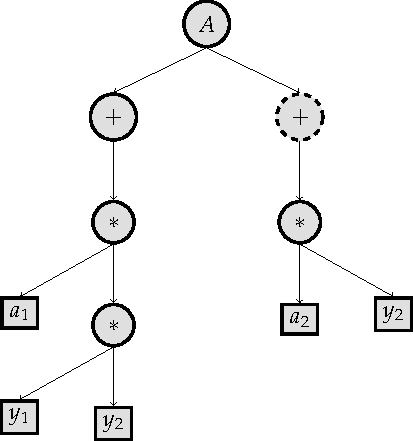
\includegraphics[width=0.4\textwidth]{"figures/cross_equation_1.pdf"}
                  \qquad
                  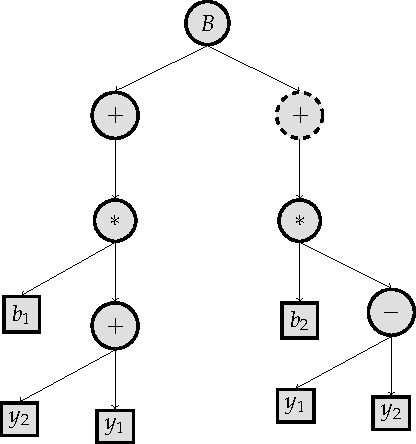
\includegraphics[width=0.4\textwidth]{"figures/cross_equation_2.pdf"}
                  \caption{Ejemplo de selección de un nodo en B cuando en A se selecciona el nodo representante de una ecuación.}
                  \label{tikzpicture:cross_equation}
              \end{figure}
          \end{center}

    \item Si se selecciona en A un nodo representante de un término en la ecuación i-ésima, se escoge un nodo representante de un término en la i-ésima ecuación en el sistema B. Se puede ver como ejemplo la figura \ref{tikzpicture:cross_term}.

          \begin{center}
              %   \begin{adjustbox}{width=0.4\textwidth, keepaspectratio}
              %       \begin{tikzpicture}[
              %               roundnode/.style={circle, draw, fill=gray!25, very thick, minimum size=7mm},
              %               squarednode/.style={rectangle, draw, fill=gray!25, very thick, minimum size=5mm},
              %               roundnode_dashed/.style={circle, draw, dashed, fill=gray!25, very thick, minimum size=7mm},
              %           ]
              %           % Nodes
              %           \node[roundnode]        (system)                            {$A$};

              %           \node[roundnode]        (plus_1)     [below left=of system]        {$+$};
              %           \node[roundnode_dashed]        (star_1_1)    [below=of plus_1]    {$*$};
              %           \node[squarednode]      (a_1)      [below left=of star_1_1]    {$a_1$};
              %           \node[roundnode]        (star_1_2)    [below=of star_1_1]    {$*$};
              %           \node[squarednode]      (S_star_1_2)       [below left=of star_1_2]   {$y_1$};
              %           \node[squarednode]      (I_star_1_2)      [below=of star_1_2]   {$y_2$};

              %           \node[roundnode]        (plus_2)     [below right=of system]        {$+$};
              %           \node[roundnode]        (star_2_1)    [below=of plus_2]    {$*$};
              %           \node[squarednode]      (a_2)      [below=of star_2_1]    {$a_2$};
              %           \node[squarednode]      (I_star_2_1)      [below right=of star_2_1]   {$y_2$};

              %           %Lines
              %           \draw [->] (system.south) -- (plus_1.north);
              %           \draw[->] (system.south) -- (plus_2.north);
              %           \draw[->] (plus_1.south) -- (star_1_1.north);
              %           \draw[->] (plus_2.south) -- (star_2_1.north);
              %           \draw[->] (star_1_1.south) -- (a_1.north);
              %           \draw[->] (star_1_1.south) -- (star_1_2.north);
              %           \draw[->] (star_1_2.south) -- (S_star_1_2.north);
              %           \draw[->] (star_1_2.south) -- (I_star_1_2.north);
              %           \draw[->] (star_2_1.south) -- (a_2.north);
              %           \draw[->] (star_2_1.south) -- (I_star_2_1.north);
              %       \end{tikzpicture}
              %   \end{adjustbox}
              %   \qquad
              %   \begin{adjustbox}{width=0.4\textwidth, keepaspectratio}
              %       \begin{tikzpicture}[
              %               roundnode/.style={circle, draw, fill=gray!25, very thick, minimum size=7mm},
              %               squarednode/.style={rectangle, draw, fill=gray!25, very thick, minimum size=5mm},
              %               roundnode_dashed/.style={circle, draw, dashed, fill=gray!25, very thick, minimum size=7mm},
              %           ]
              %           % Nodes
              %           \node[roundnode]        (system)                            {$B$};

              %           \node[roundnode]        (plus_1)     [below left=of system]        {$+$};
              %           \node[roundnode_dashed]        (star_1_1)    [below=of plus_1]    {$*$};
              %           \node[squarednode]      (a_3)      [below left=of star_1_1]    {$b_1$};
              %           \node[roundnode]        (plus_1_2)    [below=of star_1_1]    {$+$};
              %           \node[squarednode]      (I_plus_1_2)       [below left=of plus_1_2]   {$y_2$};
              %           \node[squarednode]      (S_plus_1_2)      [below=of plus_1_2]   {$y_1$};

              %           \node[roundnode]        (plus_2)     [below right=of system]        {$+$};
              %           \node[roundnode]        (star_2_1)    [below=of plus_2]    {$*$};
              %           \node[squarednode]      (a_4)      [below=of star_2_1]    {$b_2$};
              %           \node[roundnode]        (sub_2_1)    [below right=of star_2_1]    {$-$};
              %           \node[squarednode]      (S_sub_2_1)       [below left=of sub_2_1]   {$y_1$};
              %           \node[squarednode]      (I_sub_2_1)      [below=of sub_2_1]   {$y_2$};

              %           %Lines
              %           \draw [->] (system.south) -- (plus_1.north);
              %           \draw[->] (system.south) -- (plus_2.north);
              %           \draw[->] (plus_1.south) -- (star_1_1.north);
              %           \draw[->] (plus_2.south) -- (star_2_1.north);
              %           \draw[->] (star_1_1.south) -- (a_3.north);
              %           \draw[->] (star_1_1.south) -- (plus_1_2.north);
              %           \draw[->] (plus_1_2.south) -- (I_plus_1_2.north);
              %           \draw[->] (plus_1_2.south) -- (S_plus_1_2.north);
              %           \draw[->] (star_2_1.south) -- (a_4.north);
              %           \draw[->] (star_2_1.south) -- (sub_2_1.north);
              %           \draw[->] (sub_2_1.south) -- (S_sub_2_1.north);
              %           \draw[->] (sub_2_1.south) -- (I_sub_2_1.north);
              %       \end{tikzpicture}
              %   \end{adjustbox}
              \begin{figure}[h]
                  \centering
                  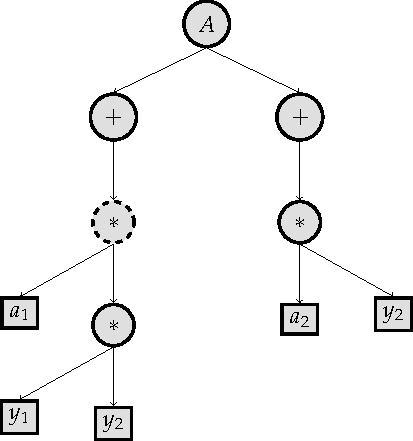
\includegraphics[width=0.4\textwidth]{"figures/cross_term_1.pdf"}
                  \qquad
                  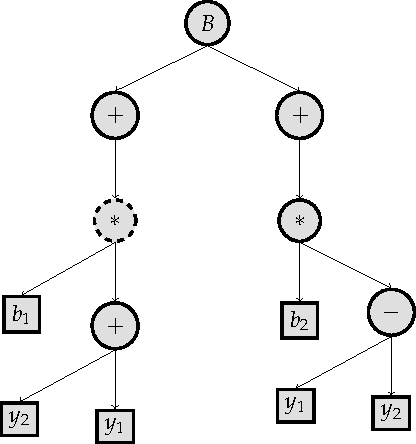
\includegraphics[width=0.4\textwidth]{"figures/cross_term_2.pdf"}
                  \caption{Ejemplo de selección de un nodo en B cuando en A se selecciona el nodo representante de un término en la primera ecuación.}
                  \label{tikzpicture:cross_term}
              \end{figure}
          \end{center}


    \item Si el nodo seleccionado en A es el representante de una operación o una variable perteneciente a la i-ésima ecuación, se selecciona un nodo representante de una operación o una variable que pertenezca a algún término en la i-ésima ecuación en el sistema B. Se puede ver como ejemplo la figura \ref{tikzpicture:cross_operation}.

          \begin{center}
              %   \begin{adjustbox}{width=0.4\textwidth, keepaspectratio}
              %       \begin{tikzpicture}[
              %               roundnode/.style={circle, draw, fill=gray!25, very thick, minimum size=7mm},
              %               squarednode/.style={rectangle, draw, fill=gray!25, very thick, minimum size=5mm},
              %               squarednode_dashed/.style={rectangle, draw, dashed, fill=gray!25, very thick, minimum size=7mm},
              %           ]
              %           % Nodes
              %           \node[roundnode]        (system)                            {$A$};

              %           \node[roundnode]        (plus_1)     [below left=of system]        {$+$};
              %           \node[roundnode]        (star_1_1)    [below=of plus_1]    {$*$};
              %           \node[squarednode]      (a_1)      [below left=of star_1_1]    {$a_1$};
              %           \node[roundnode]        (star_1_2)    [below=of star_1_1]    {$*$};
              %           \node[squarednode]      (S_star_1_2)       [below left=of star_1_2]   {$y_1$};
              %           \node[squarednode]      (I_star_1_2)      [below=of star_1_2]   {$y_2$};

              %           \node[roundnode]        (plus_2)     [below right=of system]        {$+$};
              %           \node[roundnode]        (star_2_1)    [below=of plus_2]    {$*$};
              %           \node[squarednode]      (a_2)      [below=of star_2_1]    {$a_2$};
              %           \node[squarednode_dashed]      (I_star_2_1)      [below right=of star_2_1]   {$y_2$};

              %           %Lines
              %           \draw [->] (system.south) -- (plus_1.north);
              %           \draw[->] (system.south) -- (plus_2.north);
              %           \draw[->] (plus_1.south) -- (star_1_1.north);
              %           \draw[->] (plus_2.south) -- (star_2_1.north);
              %           \draw[->] (star_1_1.south) -- (a_1.north);
              %           \draw[->] (star_1_1.south) -- (star_1_2.north);
              %           \draw[->] (star_1_2.south) -- (S_star_1_2.north);
              %           \draw[->] (star_1_2.south) -- (I_star_1_2.north);
              %           \draw[->] (star_2_1.south) -- (a_2.north);
              %           \draw[->] (star_2_1.south) -- (I_star_2_1.north);
              %       \end{tikzpicture}
              %   \end{adjustbox}
              %   \qquad
              %   \begin{adjustbox}{width=0.4\textwidth, keepaspectratio}
              %       \begin{tikzpicture}[
              %               roundnode/.style={circle, draw, fill=gray!25, very thick, minimum size=7mm},
              %               squarednode/.style={rectangle, draw, fill=gray!25, very thick, minimum size=5mm},
              %               roundnode_dashed/.style={circle, draw, dashed, fill=gray!25, very thick, minimum size=7mm},
              %           ]
              %           % Nodes
              %           \node[roundnode]        (system)                            {$B$};

              %           \node[roundnode]        (plus_1)     [below left=of system]        {$+$};
              %           \node[roundnode]        (star_1_1)    [below=of plus_1]    {$*$};
              %           \node[squarednode]      (a_3)      [below left=of star_1_1]    {$b_1$};
              %           \node[roundnode]        (plus_1_2)    [below=of star_1_1]    {$+$};
              %           \node[squarednode]      (I_plus_1_2)       [below left=of plus_1_2]   {$y_2$};
              %           \node[squarednode]      (S_plus_1_2)      [below=of plus_1_2]   {$y_1$};

              %           \node[roundnode]        (plus_2)     [below right=of system]        {$+$};
              %           \node[roundnode]        (star_2_1)    [below=of plus_2]    {$*$};
              %           \node[squarednode]      (a_4)      [below=of star_2_1]    {$b_2$};
              %           \node[roundnode_dashed]        (sub_2_1)    [below right=of star_2_1]    {$-$};
              %           \node[squarednode]      (S_sub_2_1)       [below left=of sub_2_1]   {$y_1$};
              %           \node[squarednode]      (I_sub_2_1)      [below=of sub_2_1]   {$y_2$};

              %           %Lines
              %           \draw [->] (system.south) -- (plus_1.north);
              %           \draw[->] (system.south) -- (plus_2.north);
              %           \draw[->] (plus_1.south) -- (star_1_1.north);
              %           \draw[->] (plus_2.south) -- (star_2_1.north);
              %           \draw[->] (star_1_1.south) -- (a_3.north);
              %           \draw[->] (star_1_1.south) -- (plus_1_2.north);
              %           \draw[->] (plus_1_2.south) -- (I_plus_1_2.north);
              %           \draw[->] (plus_1_2.south) -- (S_plus_1_2.north);
              %           \draw[->] (star_2_1.south) -- (a_4.north);
              %           \draw[->] (star_2_1.south) -- (sub_2_1.north);
              %           \draw[->] (sub_2_1.south) -- (S_sub_2_1.north);
              %           \draw[->] (sub_2_1.south) -- (I_sub_2_1.north);
              %       \end{tikzpicture}
              %   \end{adjustbox}
              \begin{figure}[H]
                  \centering
                  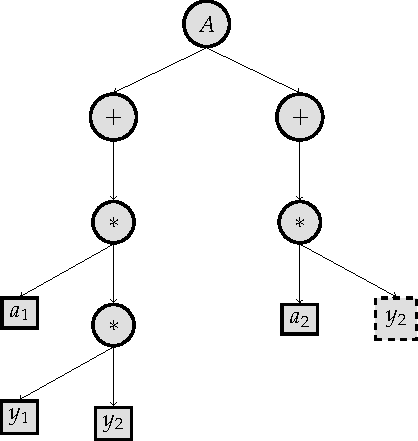
\includegraphics[width=0.37\textwidth]{"figures/cross_operation_1.pdf"}
                  \qquad
                  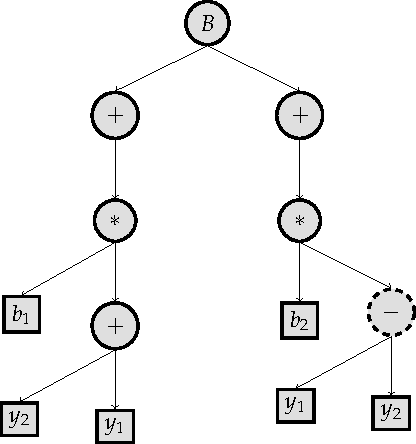
\includegraphics[width=0.37\textwidth]{"figures/cross_operation_2.pdf"}
                  \caption{Ejemplo de selección de un nodo en B cuando en A se selecciona el nodo representante de una variable en la segunda ecuación.}
                  \label{tikzpicture:cross_operation}
              \end{figure}
          \end{center}

\end{itemize}

Por ejemplo, si se tiene el sistema $A$:

\begin{align*}
    S' & = - a_1 * S * I         \\
    I' & = a_2 * S * I - a_3 * I \\
    R' & = a_4 * I,
\end{align*}

y el sistema B:

\begin{align*}
    S' & = b_1 * (S + I) \\
    I' & = b_2 * S * I   \\
    R' & = b_3 * S,
\end{align*}

donde su representación computacional aparece en la figura \ref{tikzpicture:cross_example_1},

\begin{center}
    % \begin{adjustbox}{width=0.5\textwidth, keepaspectratio}
    %     \begin{tikzpicture}[
    %             roundnode/.style={circle, draw, fill=gray!25, very thick, minimum size=7mm},
    %             squarednode/.style={rectangle, draw, fill=gray!25, very thick, minimum size=5mm},
    %             roundnode_dashed/.style={circle, draw, dashed, fill=gray!25, very thick, minimum size=7mm},
    %         ]
    %         % Nodes
    %         \node[roundnode]        (system)                            {$A$};

    %         \node[roundnode]        (plus_S)     [below left=of system]        {$+$};
    %         \node[roundnode]        (star_S_1)    [below left=of plus_S]    {$*$};
    %         \node[squarednode]      (alpha_star_S_1)      [below left=of star_S_1]    {$a_1$};
    %         \node[roundnode]        (neg_star_S_1)    [below=of star_S_1]    {$-$};
    %         \node[roundnode]        (star_S_2)    [below=of neg_star_S_1]    {$*$};
    %         \node[squarednode]      (S_star_S)       [below left=of star_S_2]   {$S$};
    %         \node[squarednode]      (I_star_S)      [below=of star_S_2]   {$I$};

    %         \node[roundnode_dashed]        (plus_I)     [below=of system]        {$+$};
    %         \node[roundnode]        (star_I_1)    [below left=1cm and 0.5cm of plus_I]    {$*$};
    %         \node[squarednode]      (alpha_star_I_1)      [below left=1cm and 0.5cm of star_I_1]    {$a_2$};
    %         \node[roundnode]        (star_I_2)    [below=of star_I_1]    {$*$};
    %         \node[squarednode]      (S_star_I)       [below left=1cm and 0.5cm of star_I_2]   {$S$};
    %         \node[squarednode]      (I_star_I_1)      [below=of star_I_2]   {$I$};

    %         \node[roundnode]        (star_I_3)    [below right=1cm and 0.5cm of plus_I]    {$*$};
    %         \node[squarednode]      (beta_star_I_1)      [below=of star_I_3]    {$a_3$};
    %         \node[roundnode]        (neg_star_I_1)    [below right=1cm and 0.5cm of star_I_3]    {$-$};
    %         \node[squarednode]      (I_star_I_2)      [below=of neg_star_I_1]   {$I$};

    %         \node[roundnode]        (plus_R)     [below right=of system]        {$+$};
    %         \node[roundnode]        (star_R_1)    [below right=of plus_R]    {$*$};
    %         \node[squarednode]      (beta_star_R_1)      [below=of star_R_1]    {$a_4$};
    %         \node[squarednode]      (I_star_R)      [below right=of star_R_1]   {$I$};

    %         %Lines
    %         \draw [->] (system.south) -- (plus_S.north);
    %         \draw[->] (system.south) -- (plus_I.north);
    %         \draw[->] (system.south) -- (plus_R.north);

    %         \draw[->] (plus_S.south) -- (star_S_1.north);
    %         \draw[->] (star_S_1.south) -- (alpha_star_S_1.north);
    %         \draw[->] (star_S_1.south) -- (neg_star_S_1.north);
    %         \draw[->] (neg_star_S_1.south) -- (star_S_2.north);
    %         \draw[->] (star_S_2.south) -- (S_star_S.north);
    %         \draw[->] (star_S_2.south) -- (I_star_S.north);

    %         \draw[->] (plus_I.south) -- (star_I_1.north);
    %         \draw[->] (plus_I.south) -- (star_I_3.north);
    %         \draw[->] (star_I_1.south) -- (alpha_star_I_1.north);
    %         \draw[->] (star_I_1.south) -- (star_I_2.north);
    %         \draw[->] (star_I_2.south) -- (S_star_I.north);
    %         \draw[->] (star_I_2.south) -- (I_star_I_1.north);

    %         \draw[->] (star_I_3.south) -- (beta_star_I_1.north);
    %         \draw[->] (star_I_3.south) -- (neg_star_I_1.north);
    %         \draw[->] (neg_star_I_1.south) -- (I_star_I_2.north);

    %         \draw[->] (plus_R.south) -- (star_R_1.north);
    %         \draw[->] (star_R_1.south) -- (beta_star_R_1.north);
    %         \draw[->] (star_R_1.south) -- (I_star_R.north);
    %     \end{tikzpicture}
    % \end{adjustbox}
    \begin{figure}[H]
        \centering
        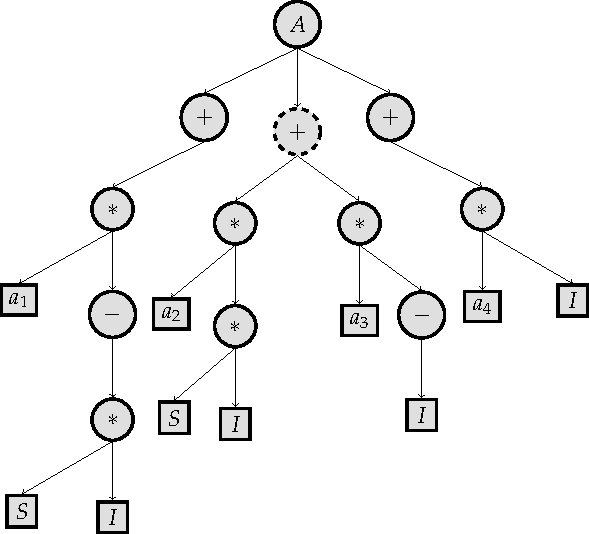
\includegraphics[width=0.47\textwidth]{"figures/cross_example_1.pdf"}
        \qquad
        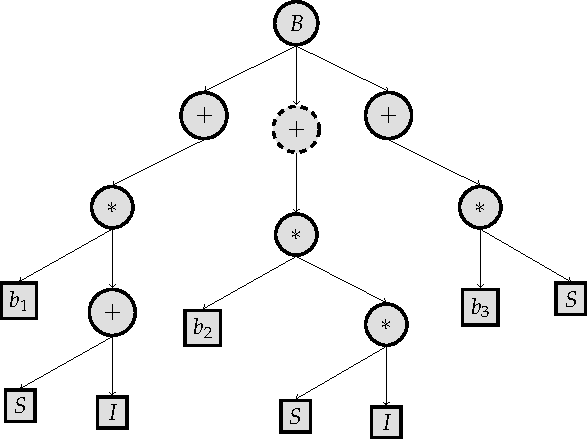
\includegraphics[width=0.47\textwidth]{"figures/cross_example_2.pdf"}
        \caption{Representación en forma de árboles de los sistemas A y B.}
        \label{tikzpicture:cross_example_1}
    \end{figure}
\end{center}

% \begin{center}
%     \begin{adjustbox}{width=0.5\textwidth, keepaspectratio}
%         \begin{tikzpicture}[
%                 roundnode/.style={circle, draw, fill=gray!25, very thick, minimum size=7mm},
%                 squarednode/.style={rectangle, draw, fill=gray!25, very thick, minimum size=5mm},
%                 roundnode_dashed/.style={circle, draw, dashed, fill=gray!25, very thick, minimum size=7mm},
%             ]
%             % Nodes
%             \node[roundnode]        (system)                            {$B$};

%             \node[roundnode]        (plus_S)     [below left=of system]        {$+$};
%             \node[roundnode]        (star_S_1)    [below left=of plus_S]    {$*$};
%             \node[squarednode]      (alpha_star_S_1)      [below left=of star_S_1]    {$b_1$};
%             \node[roundnode]        (add_S_2)    [below=of star_S_1]    {$+$};
%             \node[squarednode]      (S_star_S)       [below left=of add_S_2]   {$S$};
%             \node[squarednode]      (I_star_S)      [below=of add_S_2]   {$I$};

%             \node[roundnode_dashed]        (plus_I)     [below=of system]        {$+$};
%             \node[roundnode]        (star_I_1)    [below=of plus_I]    {$*$};
%             \node[squarednode]      (alpha_star_I_1)      [below left=of star_I_1]    {$b_2$};
%             \node[roundnode]        (star_I_2)    [below right=of star_I_1]    {$*$};
%             \node[squarednode]      (S_star_I)       [below left=of star_I_2]   {$S$};
%             \node[squarednode]      (I_star_I_1)      [below=of star_I_2]   {$I$};

%             \node[roundnode]        (plus_R)     [below right=of system]        {$+$};
%             \node[roundnode]        (star_R_1)    [below right=of plus_R]    {$*$};
%             \node[squarednode]      (beta_star_R_1)      [below=of star_R_1]    {$b_3$};
%             \node[squarednode]      (S_star_R)      [below right=of star_R_1]   {$S$};

%             %Lines
%             \draw [->] (system.south) -- (plus_S.north);
%             \draw[->] (system.south) -- (plus_I.north);
%             \draw[->] (system.south) -- (plus_R.north);

%             \draw[->] (plus_S.south) -- (star_S_1.north);
%             \draw[->] (star_S_1.south) -- (alpha_star_S_1.north);
%             \draw[->] (star_S_1.south) -- (add_S_2.north);
%             \draw[->] (add_S_2.south) -- (S_star_S.north);
%             \draw[->] (add_S_2.south) -- (I_star_S.north);

%             \draw[->] (plus_I.south) -- (star_I_1.north);
%             \draw[->] (star_I_1.south) -- (alpha_star_I_1.north);
%             \draw[->] (star_I_1.south) -- (star_I_2.north);
%             \draw[->] (star_I_2.south) -- (S_star_I.north);
%             \draw[->] (star_I_2.south) -- (I_star_I_1.north);

%             \draw[->] (plus_R.south) -- (star_R_1.north);
%             \draw[->] (star_R_1.south) -- (beta_star_R_1.north);
%             \draw[->] (star_R_1.south) -- (S_star_R.north);
%         \end{tikzpicture}
%     \end{adjustbox}
% \end{center}

y como resultado de la operación de cruzamiento se seleccionan los nodos que se resaltan con líneas discontinuas en la figura \ref{tikzpicture:cross_example_1}, entonces el sistema resultante $C$ sería:

\begin{align*}
    S' & = - a_1 * S * I \\
    I' & = b_2 * S * I   \\
    R' & = a_4 * I,
\end{align*}

que se representa con el árbol computacional que aparece en la figura \ref{tikzpicture:cross_example_2}.

\begin{center}
    % \begin{adjustbox}{width=0.5\textwidth, keepaspectratio}
    %     \begin{tikzpicture}[
    %             roundnode/.style={circle, draw, fill=gray!25, very thick, minimum size=7mm},
    %             squarednode/.style={rectangle, draw, fill=gray!25, very thick, minimum size=5mm},
    %             roundnode_dashed/.style={circle, draw, dashed, fill=gray!25, very thick, minimum size=7mm},
    %         ]
    %         % Nodes
    %         \node[roundnode]        (system)                            {$C$};

    %         \node[roundnode]        (plus_S)     [below left=of system]        {$+$};
    %         \node[roundnode]        (star_S_1)    [below left=of plus_S]    {$*$};
    %         \node[squarednode]      (alpha_star_S_1)      [below left=of star_S_1]    {$c_1$};
    %         \node[roundnode]        (neg_star_S_1)    [below=of star_S_1]    {$-$};
    %         \node[roundnode]        (star_S_2)    [below=of neg_star_S_1]    {$*$};
    %         \node[squarednode]      (S_star_S)       [below left=of star_S_2]   {$S$};
    %         \node[squarednode]      (I_star_S)      [below=of star_S_2]   {$I$};

    %         \node[roundnode_dashed]        (plus_I)     [below=of system]        {$+$};
    %         \node[roundnode]        (star_I_1)    [below=of plus_I]    {$*$};
    %         \node[squarednode]      (alpha_star_I_1)      [below left=of star_I_1]    {$c_2$};
    %         \node[roundnode]        (star_I_2)    [below right=of star_I_1]    {$*$};
    %         \node[squarednode]      (S_star_I)       [below left=of star_I_2]   {$S$};
    %         \node[squarednode]      (I_star_I_1)      [below=of star_I_2]   {$I$};

    %         \node[roundnode]        (plus_R)     [below right=of system]        {$+$};
    %         \node[roundnode]        (star_R_1)    [below right=of plus_R]    {$*$};
    %         \node[squarednode]      (beta_star_R_1)      [below=of star_R_1]    {$c_3$};
    %         \node[squarednode]      (I_star_R)      [below right=of star_R_1]   {$I$};

    %         %Lines
    %         \draw [->] (system.south) -- (plus_S.north);
    %         \draw[->] (system.south) -- (plus_I.north);
    %         \draw[->] (system.south) -- (plus_R.north);

    %         \draw[->] (plus_S.south) -- (star_S_1.north);
    %         \draw[->] (star_S_1.south) -- (alpha_star_S_1.north);
    %         \draw[->] (star_S_1.south) -- (neg_star_S_1.north);
    %         \draw[->] (neg_star_S_1.south) -- (star_S_2.north);
    %         \draw[->] (star_S_2.south) -- (S_star_S.north);
    %         \draw[->] (star_S_2.south) -- (I_star_S.north);

    %         \draw[->] (plus_I.south) -- (star_I_1.north);
    %         \draw[->] (star_I_1.south) -- (alpha_star_I_1.north);
    %         \draw[->] (star_I_1.south) -- (star_I_2.north);
    %         \draw[->] (star_I_2.south) -- (S_star_I.north);
    %         \draw[->] (star_I_2.south) -- (I_star_I_1.north);

    %         \draw[->] (plus_R.south) -- (star_R_1.north);
    %         \draw[->] (star_R_1.south) -- (beta_star_R_1.north);
    %         \draw[->] (star_R_1.south) -- (I_star_R.north);
    %     \end{tikzpicture}
    % \end{adjustbox}
    \begin{figure}[H]
        \centering
        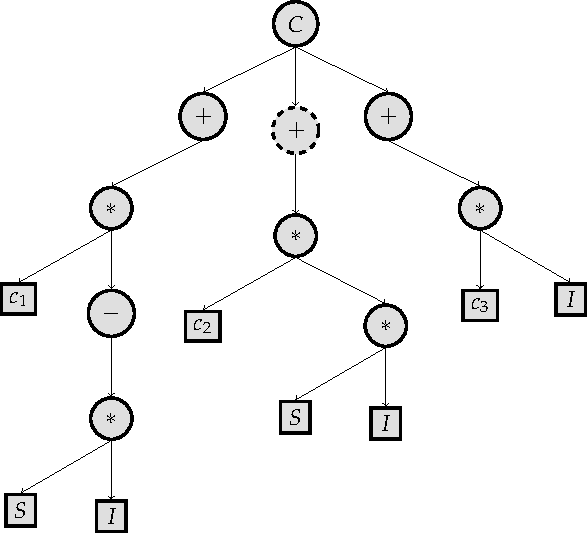
\includegraphics[width=0.6\textwidth]{"figures/cross_example_3.pdf"}
        \caption{Representación del resultado del cruzamiento entre los árboles A y B.}
        \label{tikzpicture:cross_example_2}
    \end{figure}
\end{center}

Una vez definidas las operaciones de mutación y cruzamiento solo faltaría detallar la operación de selección para tener totalmente definido el algoritmo genético. Los detalles de la última operación se presentan en la siguiente sección.

\section{Selección de las soluciones que pasan a la siguiente generación}\label{section:selection}

Dada una población inicial de $N$ individuos en una generación, se muta un subconjunto de individuos, y otro subconjunto se seleccionan para usar la operación de cruzamiento a partir de ellos. Al aplicar estas dos operaciones aparece un nuevo subconjunto de individuos. Este nuevo subconjunto se agrega a la población inicial de la generación, formando así un nuevo conjunto de individuos el cual se define como población total de la generación.

De la población total de la generación se seleccionan $M$ individuos que mejor ajustan los datos. Se seleccionan también $N - M$ individuos aleatorios con el fin de evitar mínimos locales en la búsqueda del mejor sistema. En total se selecciona de la población total de la generación una cantidad igual a la presente en la población inicial de la generación. Los valores de $N$ y $M$ que se utilizaron durante los experimentos que aparecen en el capítulo \ref{chapter:results} son 100 y 10, respectivamente.

Como resultado de la selección se obtiene una nueva población que será la población de la siguiente generación. Las operaciones de mutación y cruzamiento de la población inicial y luego selección de individuos se repiten un número fijo de veces que se define mediante el parámetro cantidad de generaciones. Esta repetición se realiza con el fin de generar varias generaciones intentando obtener mejores soluciones cada vez.

En este capítulo se describió cómo representar, mediante árboles, un sistema de EDOs lineal con respecto a los parámetros, cómo calcular su costo para un conjunto de datos, así como la forma de cruzar y mutar estos sistemas. Con estos elementos se puede definir un algoritmo genético para determinar el sistema de EDOs lineal con respecto a los parámetros que mejor describa un conjunto de datos.

En el siguiente capítulo se muestran los resultados obtenidos de aplicar este algoritmo.
\include{MainMatter/Background}
\chapter{Experimentos y resultados}\label{chapter:results}

En este capítulo se presentan los experimentos realizados para evaluar el desempeño y los resultados de la regresión simbólica propuesta en este trabajo.

En la sección \ref{section:experimental_considerations} se menciona cómo se diseñó el marco experimental para realizar distintos experimentos. En \ref{section:experimental_frame} se plantea la forma en la que se generaron los datos utilizados en los distintos experimentos y cómo se modeló la presencia de ruido en las muestras. En la sección \ref{section:experiments} se desarrollan los experimentos realizados y se aprecian sus resultados. En \ref{section:experiments_results} se analizan los resultados obtenido. A continuación se describen detalles acerca del diseño del marco experimental que se utilizó en la realización de los experimentos.

\section{Consideraciones de la etapa de experimentación}\label{section:experimental_considerations}

El espacio de búsqueda en la regresión simbólica que se propone en este trabajo comprende a todos los sistemas de ecuaciones diferenciales lineales con respecto a los parámetros donde la cantidad de ecuaciones se define según los datos. La regresión simbólica es un problema NP-difícil por lo que resulta computacionalmente costoso. Para lidiar con este costo computacional se diseñó un marco experimental que fuese factible de ejecutar en un ordenador portátil. El equipo de cómputo donde se realizaron los experimentos posee las siguientes propiedades.

\begin{itemize}
    \item \textbf{Procesador}: 11th Gen intel i9-11900H @ 2.50GHz
    \item \textbf{RAM}: 40GB
    \item \textbf{Arquitectura}: 64 bits
\end{itemize}

La implementación de la solución se desarrolla en el lenguaje de programación \emph{Python} auxiliado por bibliotecas como \emph{numpy} \cite{harris2020array} y \emph{scipy} \cite{2020SciPy-NMeth}.

Como métrica para evaluar la calidad de la solución generada por la regresión simbólica se utiliza el error cuadrático medio. Menores valores de esta métrica implica que el valor de los datos evaluados en el sistema obtenido en la regresión simbólica se acercan a los datos observados.

Cada experimento que aparece en la sección \ref{section:experiments} se realizó 30 veces y se plantea el valor promedio que obtuvo la métrica utilizada en las 30 ejecuciones del experimento. Además se indica el valor mínimo y máximo que alcanzó la métrica a lo largo de los 30 experimentos. De igual forma se plantea cuántas veces en la realización de los 30 experimentos, el método de regresión simbólica encontró un sistema igual al tomado para generar los datos.

En la siguiente sección se detalla mejor cómo se generan los datos para realizar los distintos experimentos.

\section{Descripción del marco experimental}\label{section:experimental_frame}

Los experimentos inician con la selección de un modelo conocido $f$, por ejemplo el modelo SIR:

\begin{align*}
    S' & = - aIS    \\
    I' & = aIS - bI \\
    R' & = bI.
\end{align*}

El sistema de ecuaciones diferenciales se integra en un intervalo que se define mediante parámetros y se obtiene un conjunto de puntos que representan el valor de las distintas variables a lo largo del tiempo. Por ejemplo, si se integra el modelo SIR utilizando como parámetros $a = 0.0003$, $b = 0.1$ y con $0 \leq t \leq 20$ se obtienen las curvas en la imagen \ref{fig:SIR} de la página \pageref{fig:SIR}.

\begin{figure}[h]
    \centering
    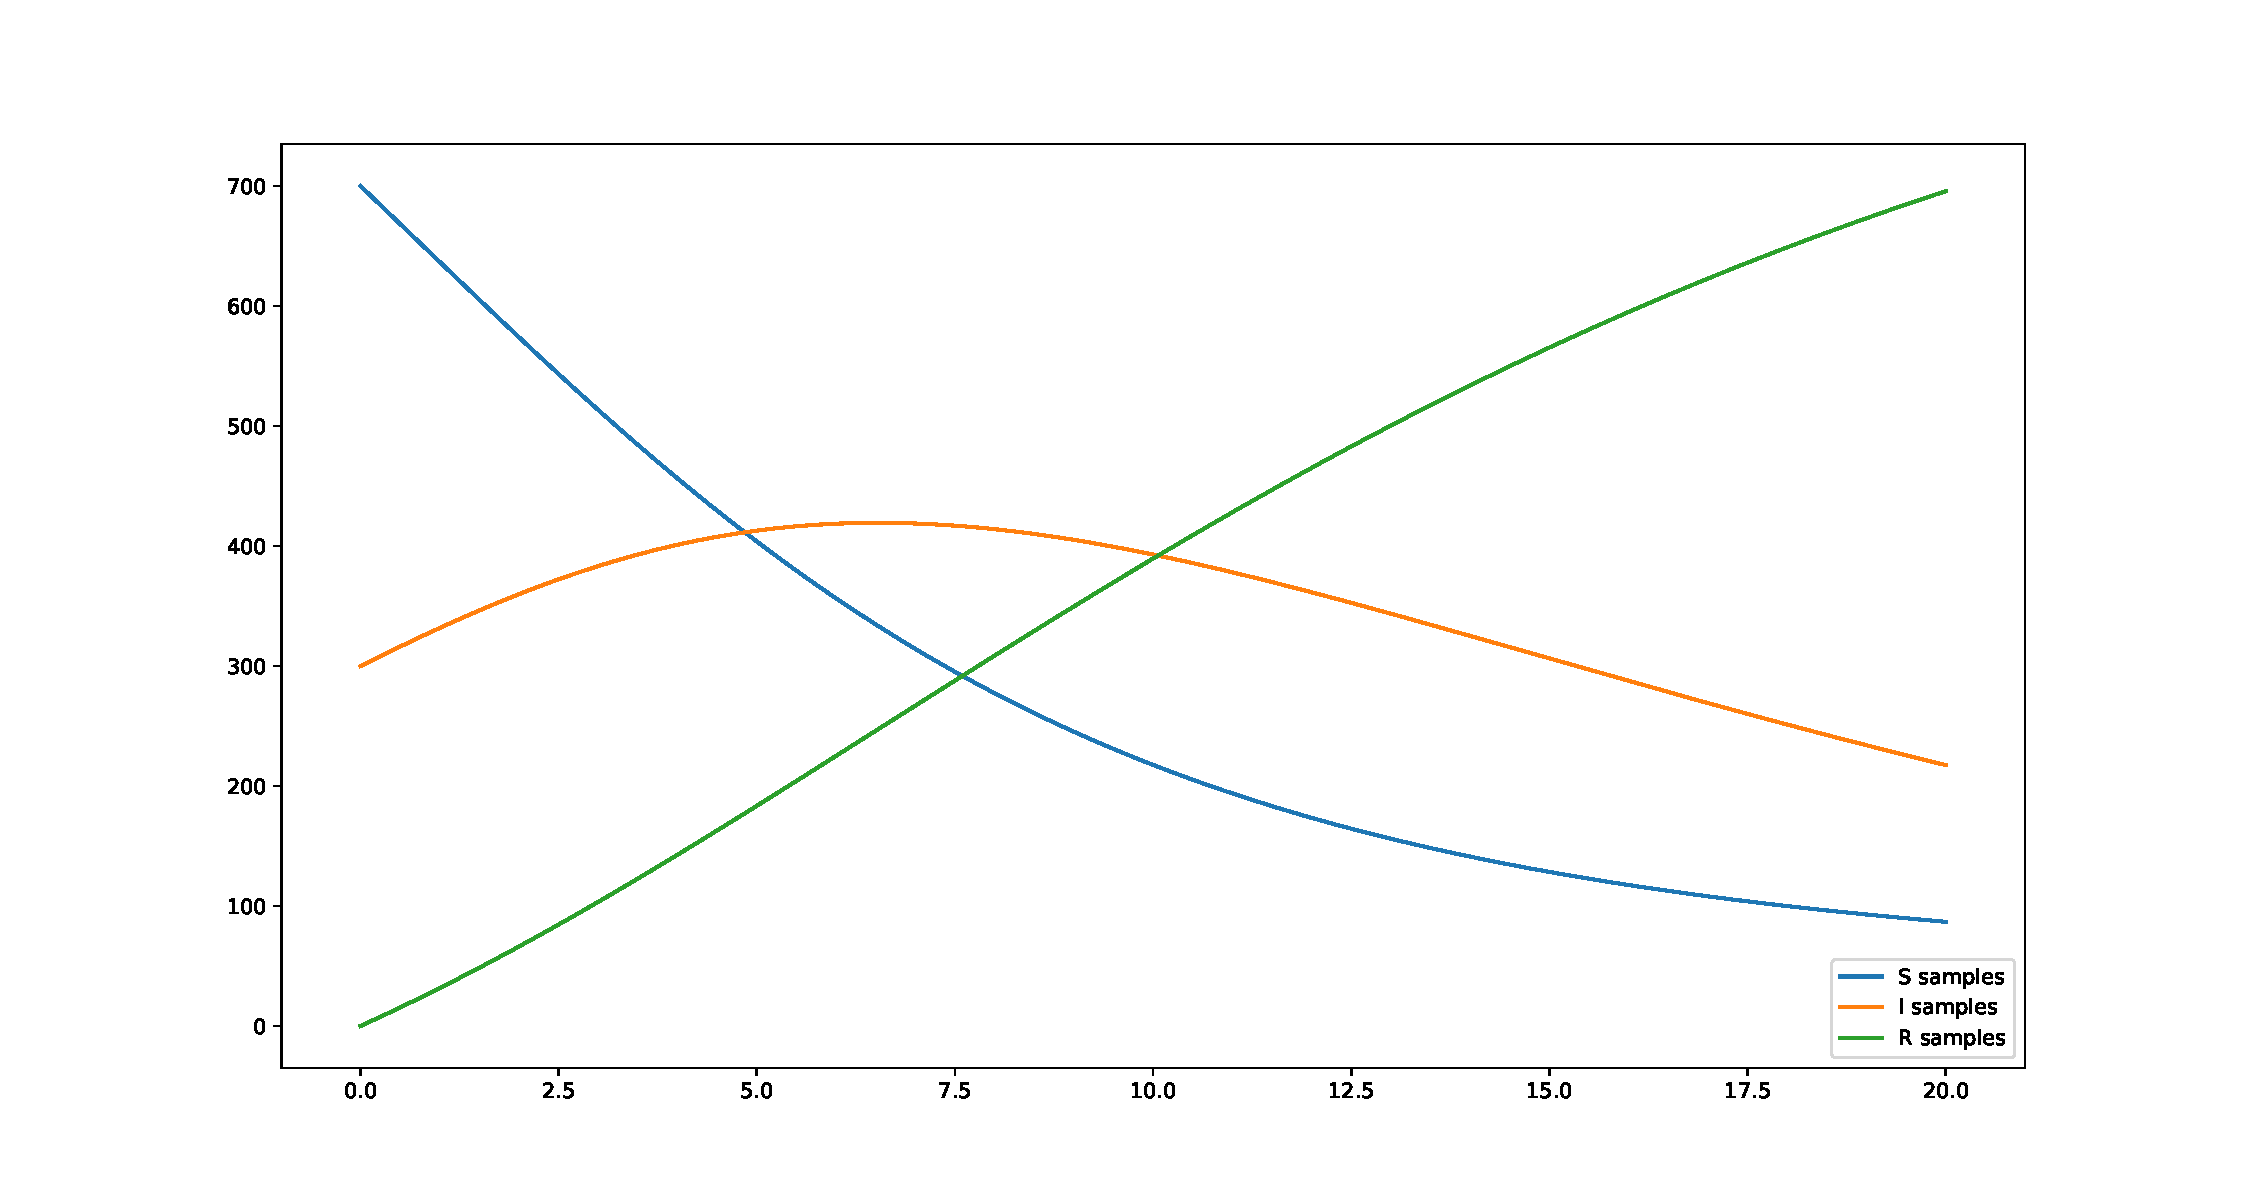
\includegraphics[width=\textwidth]{"figures/SIR.pdf"}
    \caption{modelo SIR con $a = 0.0003$, $b = 0.1$.}
    \label{fig:SIR}
\end{figure}

Cuando se tienen los datos de la forma $\{(t_i, y_i), i=1, \dots, n\}$ generados por la integración del modelo, se le agregan distintos valores de ruido a los puntos. A cada muestra $y_i$ se le agrega un valor de ruido utilizando la fórmula:

$$y_{i_{noise}} = y_i + y_i * max\_noise * random\_standard\_normal(),$$

donde $random\_standard\_normal()$ es una función que genera valores aleatorios normales, independientes, con media 0 y varianza 1. $Max\_noise$ es un parámetro con mínimo valor $0$ y máximo $1$ que define el ``ruido  máximo'' que se le agrega a cada muestra. Se puede ver el parámetro $max\_noise$ como el \% máximo del valor de cada muestra que se puede agregar como ruido. Durante los distintos experimentos se utilizaron como máximo ruido los valores de 0\%, 5\% o 10\% con respecto a cada muestra. Por ejemplo, si se agrega ruido a los datos obtenidos de la integración del sistema SIR utilizando el parámetro $max\_noise$ con valor $0.1$, se tendrían las curvas que aparecen en la imagen \ref{fig:SIR_with_noise} de la página \pageref{fig:SIR_with_noise}.

\begin{figure}[h]
    \centering
    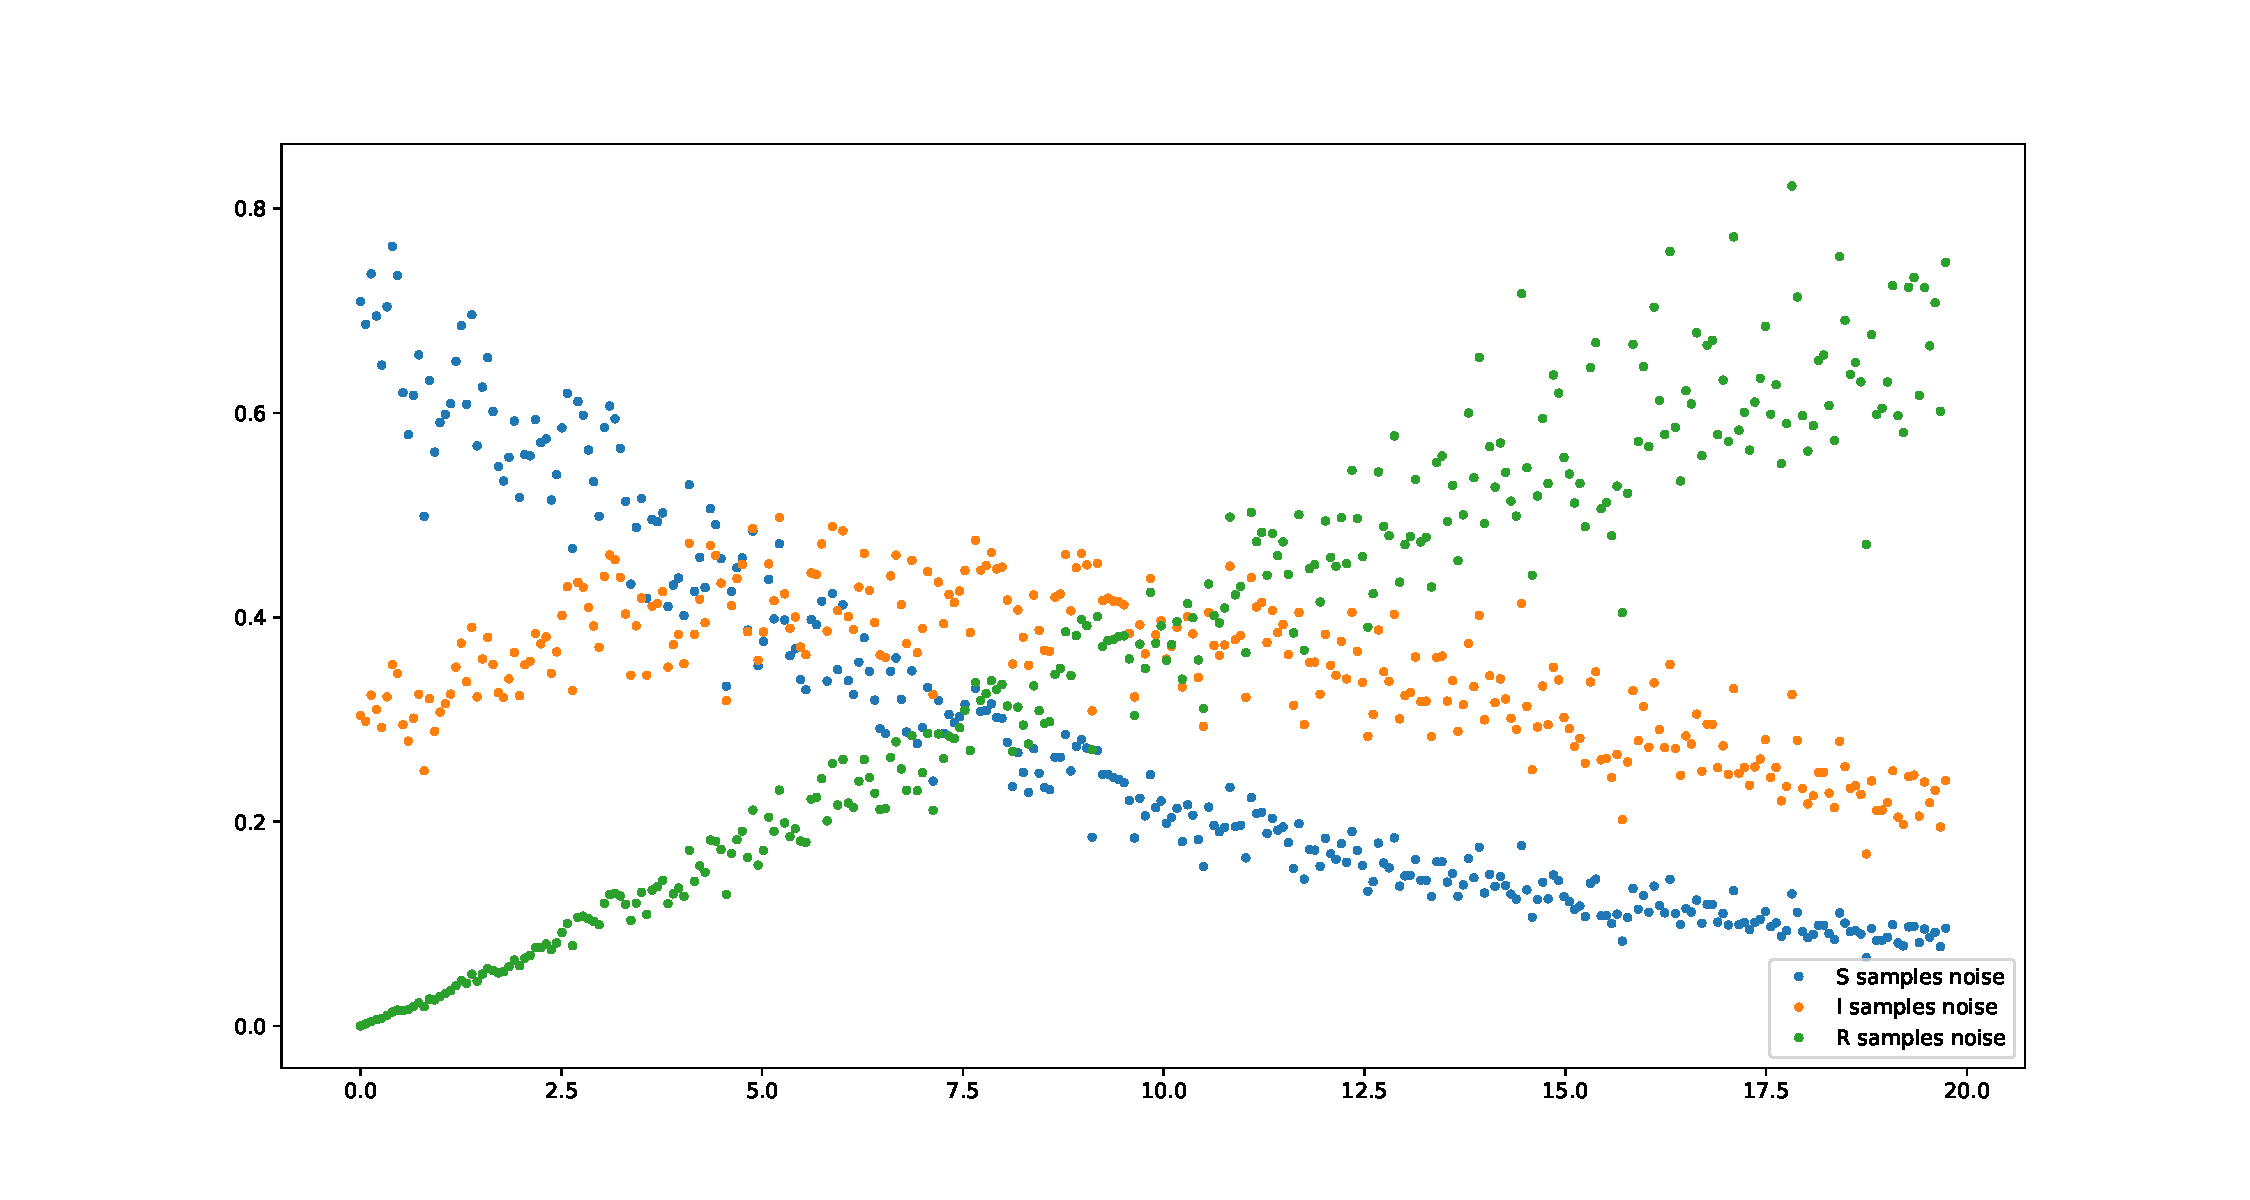
\includegraphics[width=\textwidth]{"figures/SIR_with_noise.pdf"}
    \caption{modelo SIR con $a = 0.0003$, $b = 0.1$ y $max\_noise = 0.1$.}
    \label{fig:SIR_with_noise}
\end{figure}

Cuando el valor de $max\_noise$ es mayor que 0, se usa un spline de suavizado para eliminar el ruido. El valor del parámetro de suavizado en el spline se varía para cada una de las variables. Por ejemplo, si se utiliza un spline de suavizado cúbico en los datos con ruido del sistema SIR se obtendrían las curvas que aparecen en la imagen \ref{fig:SIR_noise_with_spline} de la página \pageref{fig:SIR_noise_with_spline}.

\begin{figure}[h]
    \centering
    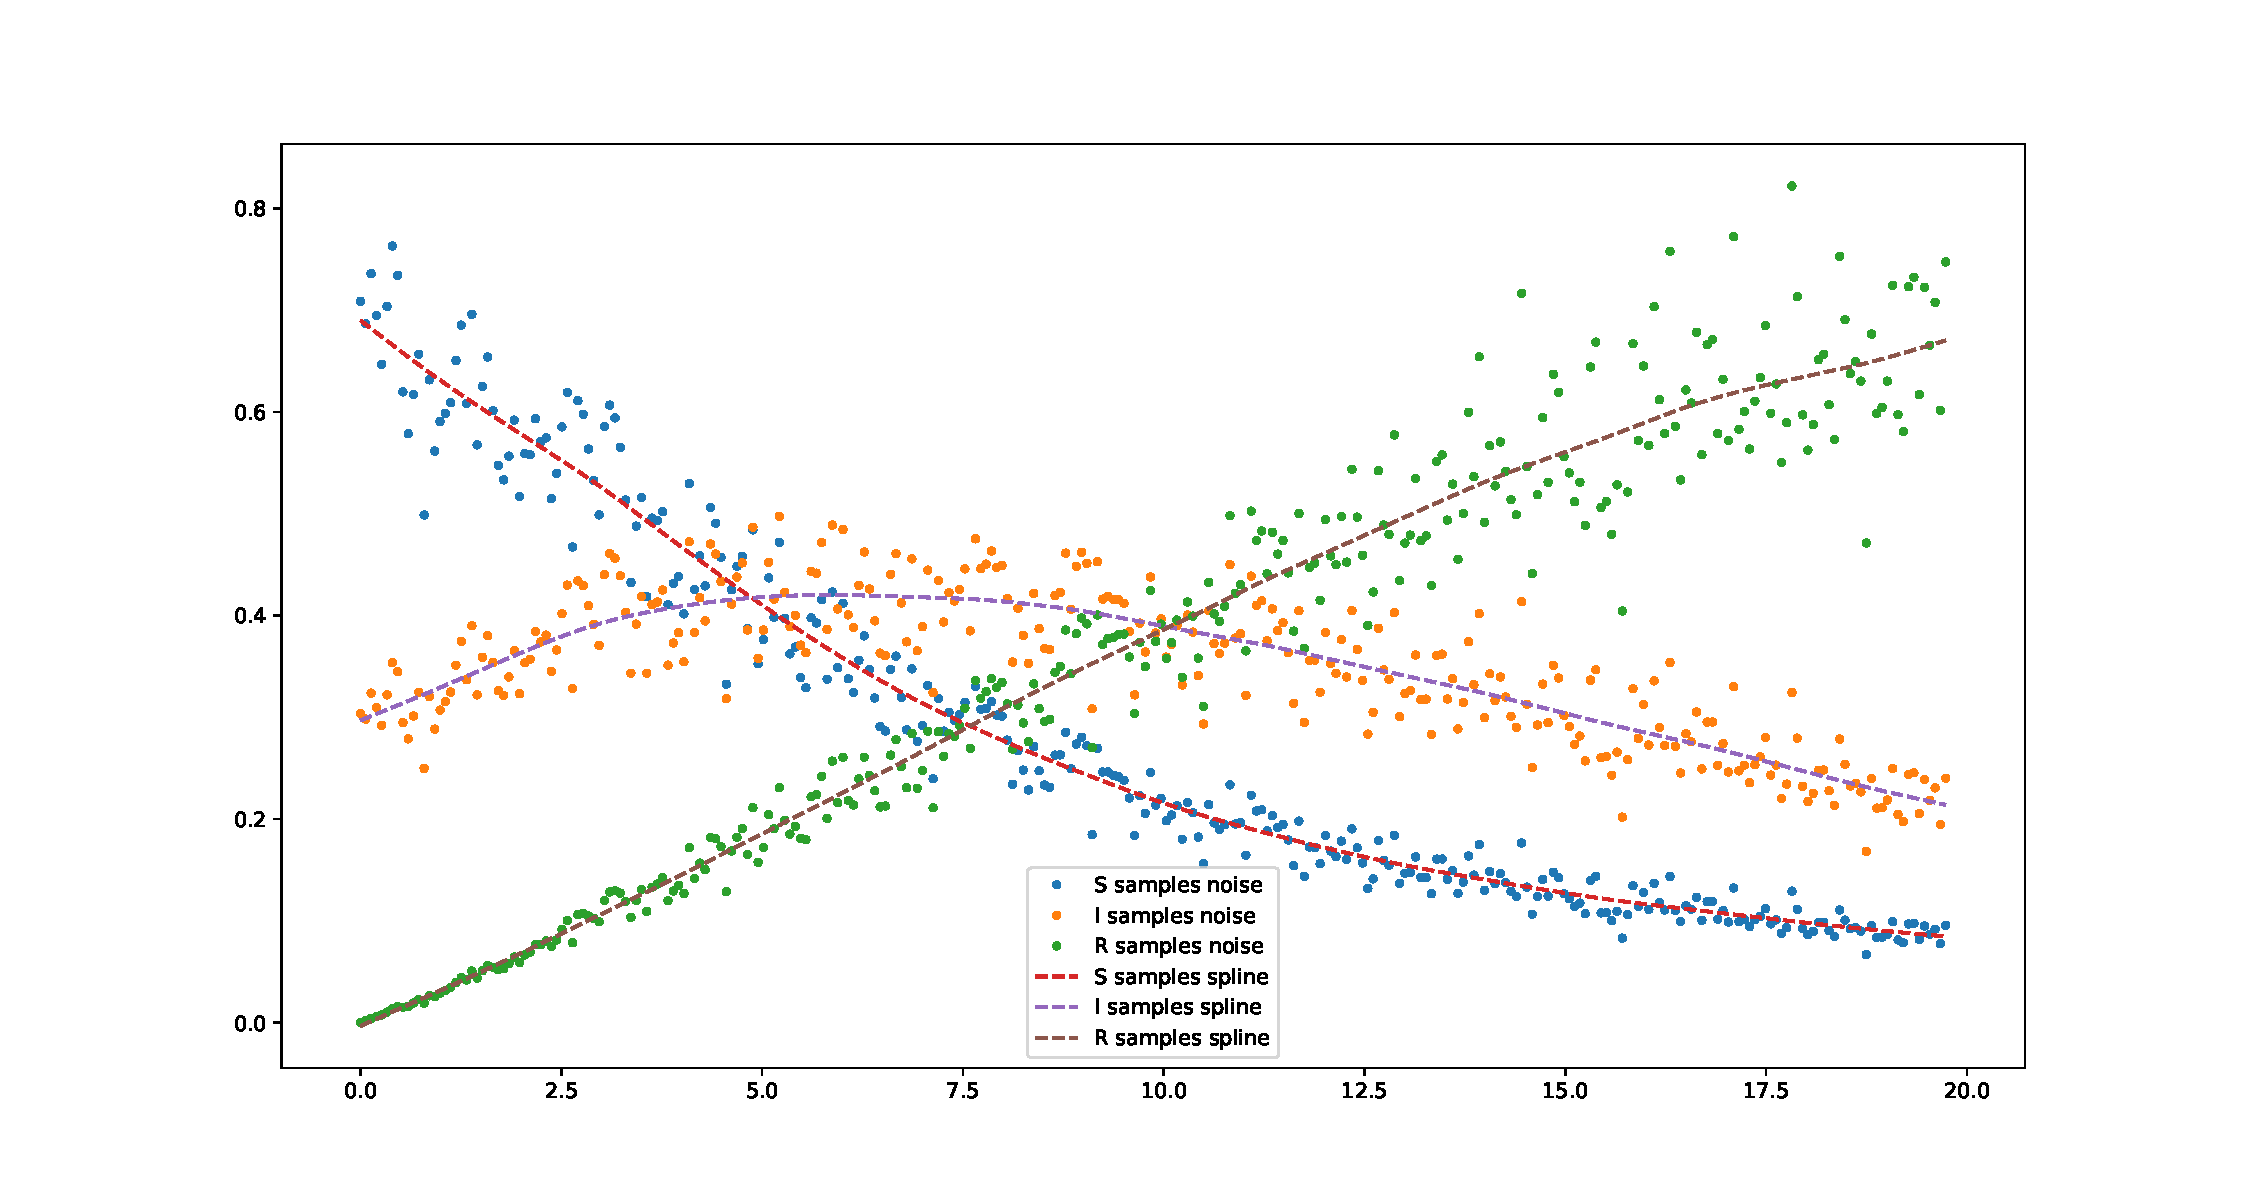
\includegraphics[width=\textwidth]{"figures/SIR_noise_with_spline.pdf"}
    \caption{modelo SIR con $a = 0.0003$, $b = 0.1$, $max\_noise = 0.1$ y smoothing-spline con valor de suavizado de $0.1$.}
    \label{fig:SIR_noise_with_spline}
\end{figure}

Una vez que se tiene el spline de suavizado, se puede aproximar el valor de la función $y_i$. Como lo que se busca es generar un conjunto de datos de la forma:

$$\{(t_i, y_i, y'_i), i=1, \dots, n\},$$

para obtener $f(t_i, y_i)$ mediante el uso de la regresión simbólica, se puede generar una aproximación del valor de $y'_i$ utilizando la primera derivada del spline.

En las siguientes secciones se presentan los experimento en los que se utiliza la regresión simbólica para encontrar el sistema de ecuaciones diferenciales lineales con respecto a los parámetros a partir de un conjunto de datos generado. Se utilizaron en total 5 modelos para la generación de los disintos conjuntos de datos que fueron el sistema de lotka volterra \cite{Hoppensteadt:2006}, SIR \cite{weiss2013sir}, SIRD \cite{bailey1975mathematical}, SIQRD \cite{molter2021mathematical} y SVVEIR \cite{kuddus2021mathematical}.

\section{Experimentos realizados}\label{section:experiments}

Todos los sistemas de ecuaciones diferenciales seleccionados para los experimentos son sistemas lineales con respecto a los parámetros. La cantidad de ecuaciones en cada uno de los modelos es distinta. De cada modelo se muestra una tabla que contiene la media del valor de la función de ajuste a lo largo de las 30 ejecuciones del experimento así como el mínimo y máximo valor que alcanzó el error cuadrático medio.

Por cada experimento en el que se utiliza el modelo $f$, se genera un conjunto de datos $S$ de la forma $\{(t_i, y_i), i=1, \dots, n\}$ mediante la integración del modelo. Luego se crea el conjunto de datos $y_{noise_{x\%}}$ resultantes de agregarle ruido al conjunto $S$ con $max\_noise=x$ y se define $y_{spline_{x\%}}$ como los datos resultantes de la aproximación de la función $y$ a partir de los datos $y_{noise_{x\%}}$. Con todos estos datos se genera el sistema $\hat{f}$ utilizando la regresión simbólica. Se define el conjunto de datos $y_{sr_{x\%}}$ como los datos generados por la integración del sistema encontrado en la regresión simbólica. Además se tiene el sistema $f_{pso}$ como el resultado de aplicar el método $PSO$ \cite{p-pso-6} utilizando el conjunto $S$.

De todos los experimentos en los que se utiliza el modelo $f$ solo se tuvieron en cuenta en los resultados un conjunto de los 30 experimentos realizado. Esta cantidad que se tiene en cuenta se define en la fila ``cantidad de sistemas'' de la tabla de resultados con la forma \ref{table:experiment_form} que aparece en la página \pageref{table:experiment_form}.

\begin{table}
    \centering
    \caption{Estructura de tabla de resultados.}
    \begin{tabular}{|c|c|}
        \hline
                             & \textbf{ruido de x\%}                                                      \\
        \hline
        cantidad de sistemas & $m$                                                                        \\
        \hline
        original             & $\frac{\frac{\sum_{i=1}^n (y_i-y_{sr_{x\%}})^2}{n}}{m}$                    \\
        \hline
        original con ruido   & $\frac{\frac{\sum_{i=1}^n (y_{noise_{x\%}}-y_{sr_{x\%}})^2}{n}}{m}$        \\
        \hline
        spline               & $\frac{\frac{\sum_{i=1}^n (y_{spline_{x\%}}-y_{sr_{x\%}})^2}{n}}{m}$       \\
        \hline
        otro método          & $\frac{\frac{\sum_{i=1}^n (f_{PSO}(t_i, y_i)-\hat{f}(t_i, y_i))^2}{n}}{m}$ \\
        \hline
    \end{tabular}
    \label{table:experiment_form}
\end{table}

A continuación se muestra el experimento realizado a partir de la generación de los datos utlizando el sistema Lotka-Volterra.

\subsection{Lotka-Volterra}

El modelo de Lotka-Volterra es un sistema utilizado para describir las interacciones entre dos especies, una como depredador y otra como presa \cite{Hoppensteadt:2006}. La población de cada especie cambia a través del tiempo de acuerdo al sistema de ecuaciones diferenciales:

\begin{align*}
    X' & = X (a - b Y)   \\
    Y' & = -Y (c - d X).
\end{align*}

Se utilizaron como valores de los parámetros $a = 0.04$, $b = 0.0005$, $c = 0.2$ y $d = 0.004$ con punto inicial $(20, 20)$ y se integró en el intervalo $0 \leq t \leq 300$ para obtener los datos que aparecen en la figura \ref{fig:lotka_volterra} de la página \pageref{fig:lotka_volterra}. Del conjunto de puntos se seleccionaron 300 muestras como datos para el método de regresión simbólica.

\begin{figure}[h]
    \centering
    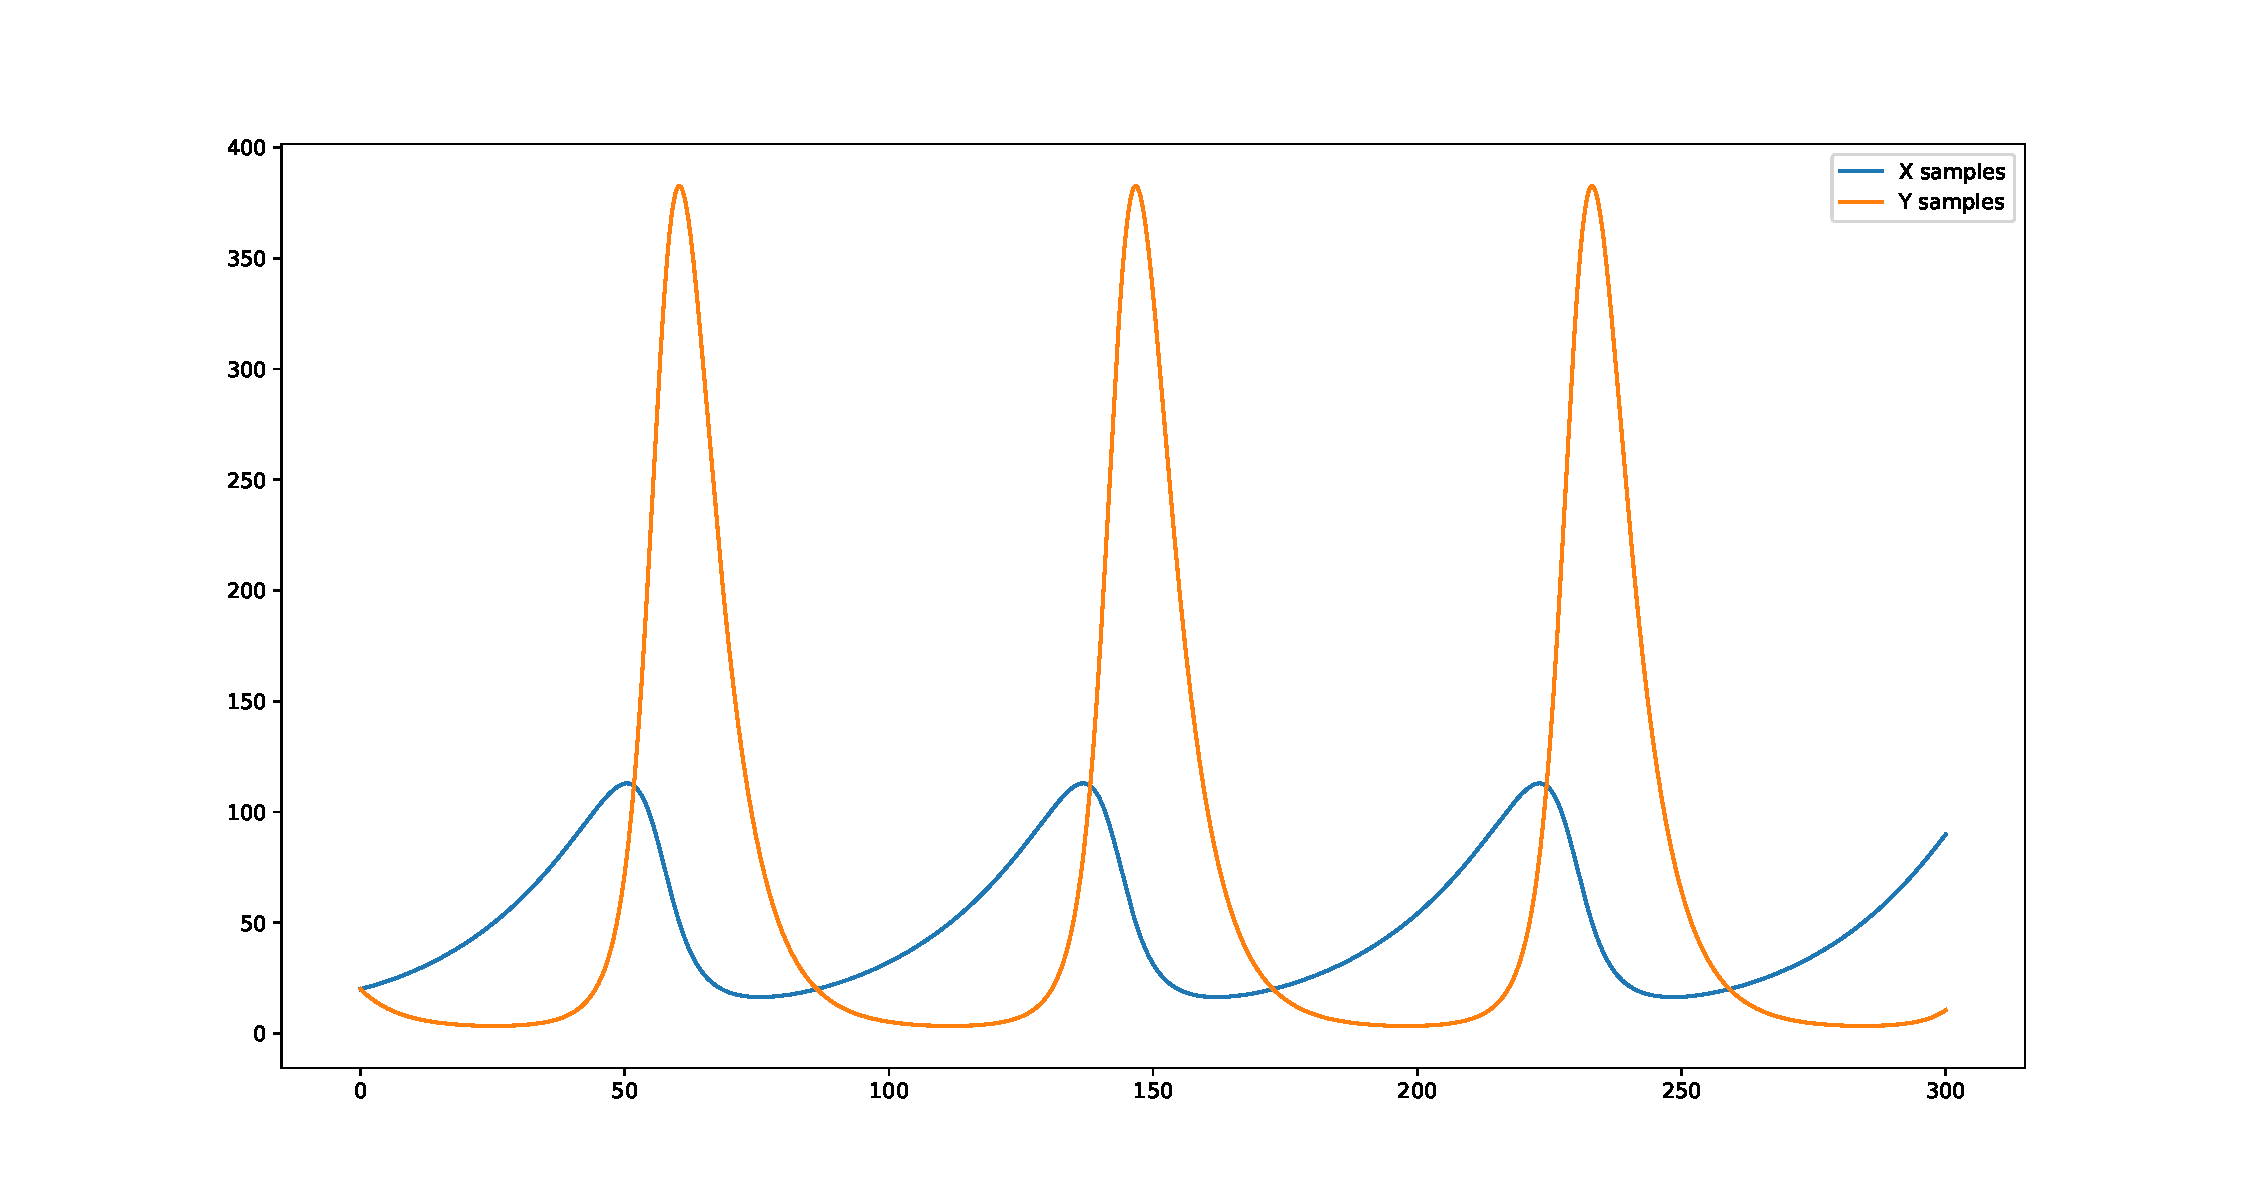
\includegraphics[width=\textwidth]{"figures/lotka_volterra.pdf"}
    \caption{modelo Lotka Volterra con $a = 0.04$, $b = 0.0005$, $c = 0.2$ y $d = 0.004$.}
    \label{fig:lotka_volterra}
\end{figure}

Los resultados que se obtienen durante las 30 ejecuciones del experimento aparecen en la tablas \ref{table:experiment_lotka_volterra}.

\begin{table}[!h]
    \centering
    \caption{Resultados que se obtienen en el modelo Lotka-Volterra.}

    \begin{tabular}{|c|c|c|c|}
        \hline
               & \textbf{ruido de 0\%} & \textbf{ruido de 5\%} & \textbf{ruido de 10\%} \\
        \hline
        media  & 0.74514               & 0.69138               & 0.84485                \\
        \hline
        mínimo & 0.28343               & 0.42189               & 0.54373                \\
        \hline
        máximo & 0.97944               & 1.11027               & 1.68603                \\
        \hline
    \end{tabular}

    \begin{tabular}{|c|c|c|c|c|c|}
        \hline
                             & \textbf{ruido de 0\%} & \textbf{ruido de 5\%} & \textbf{ruido de 10\%} \\
        \hline
        cantidad de sistemas & 30                    & 28                    & 25                     \\
        \hline
        original             & 17.01575              & 52.17101              & 50.30572               \\
        \hline
        original con ruido   & 17.01575              & 52.21558              & 50.56727               \\
        \hline
        spline               & 17.01575              & 51.85661              & 49.99422               \\
        \hline
        otro método          & 1394.26981            & 1111.95166            & 1519.66141             \\
        \hline
    \end{tabular}

    \label{table:experiment_lotka_volterra}
\end{table}

Durante la realización de los experimentos el modelo de lotka-volterra, la regresión simbólica encontró el sistema que generó los datos pero con otros parámetros en 21 ocasiones cuando no se utilizaba ruido en los datos, 13 veces cuando se utilizó un ruido máximo de 5\% y 6 veces cuando se utilizó un ruido máximo de 10\%. En las figuras \ref{fig:final_plot_LV_0.0} de la página \pageref{fig:final_plot_LV_0.0}, \ref{fig:final_plot_LV_0.05} de la página \pageref{fig:final_plot_LV_0.05} y \ref{fig:final_plot_LV_0.1} de la página \pageref{fig:final_plot_LV_0.1} se pueden ver los datos originales comparados con los datos obtenidos del mejor resultado generado por la regresión simbólica.

\begin{figure}[h]
    \centering
    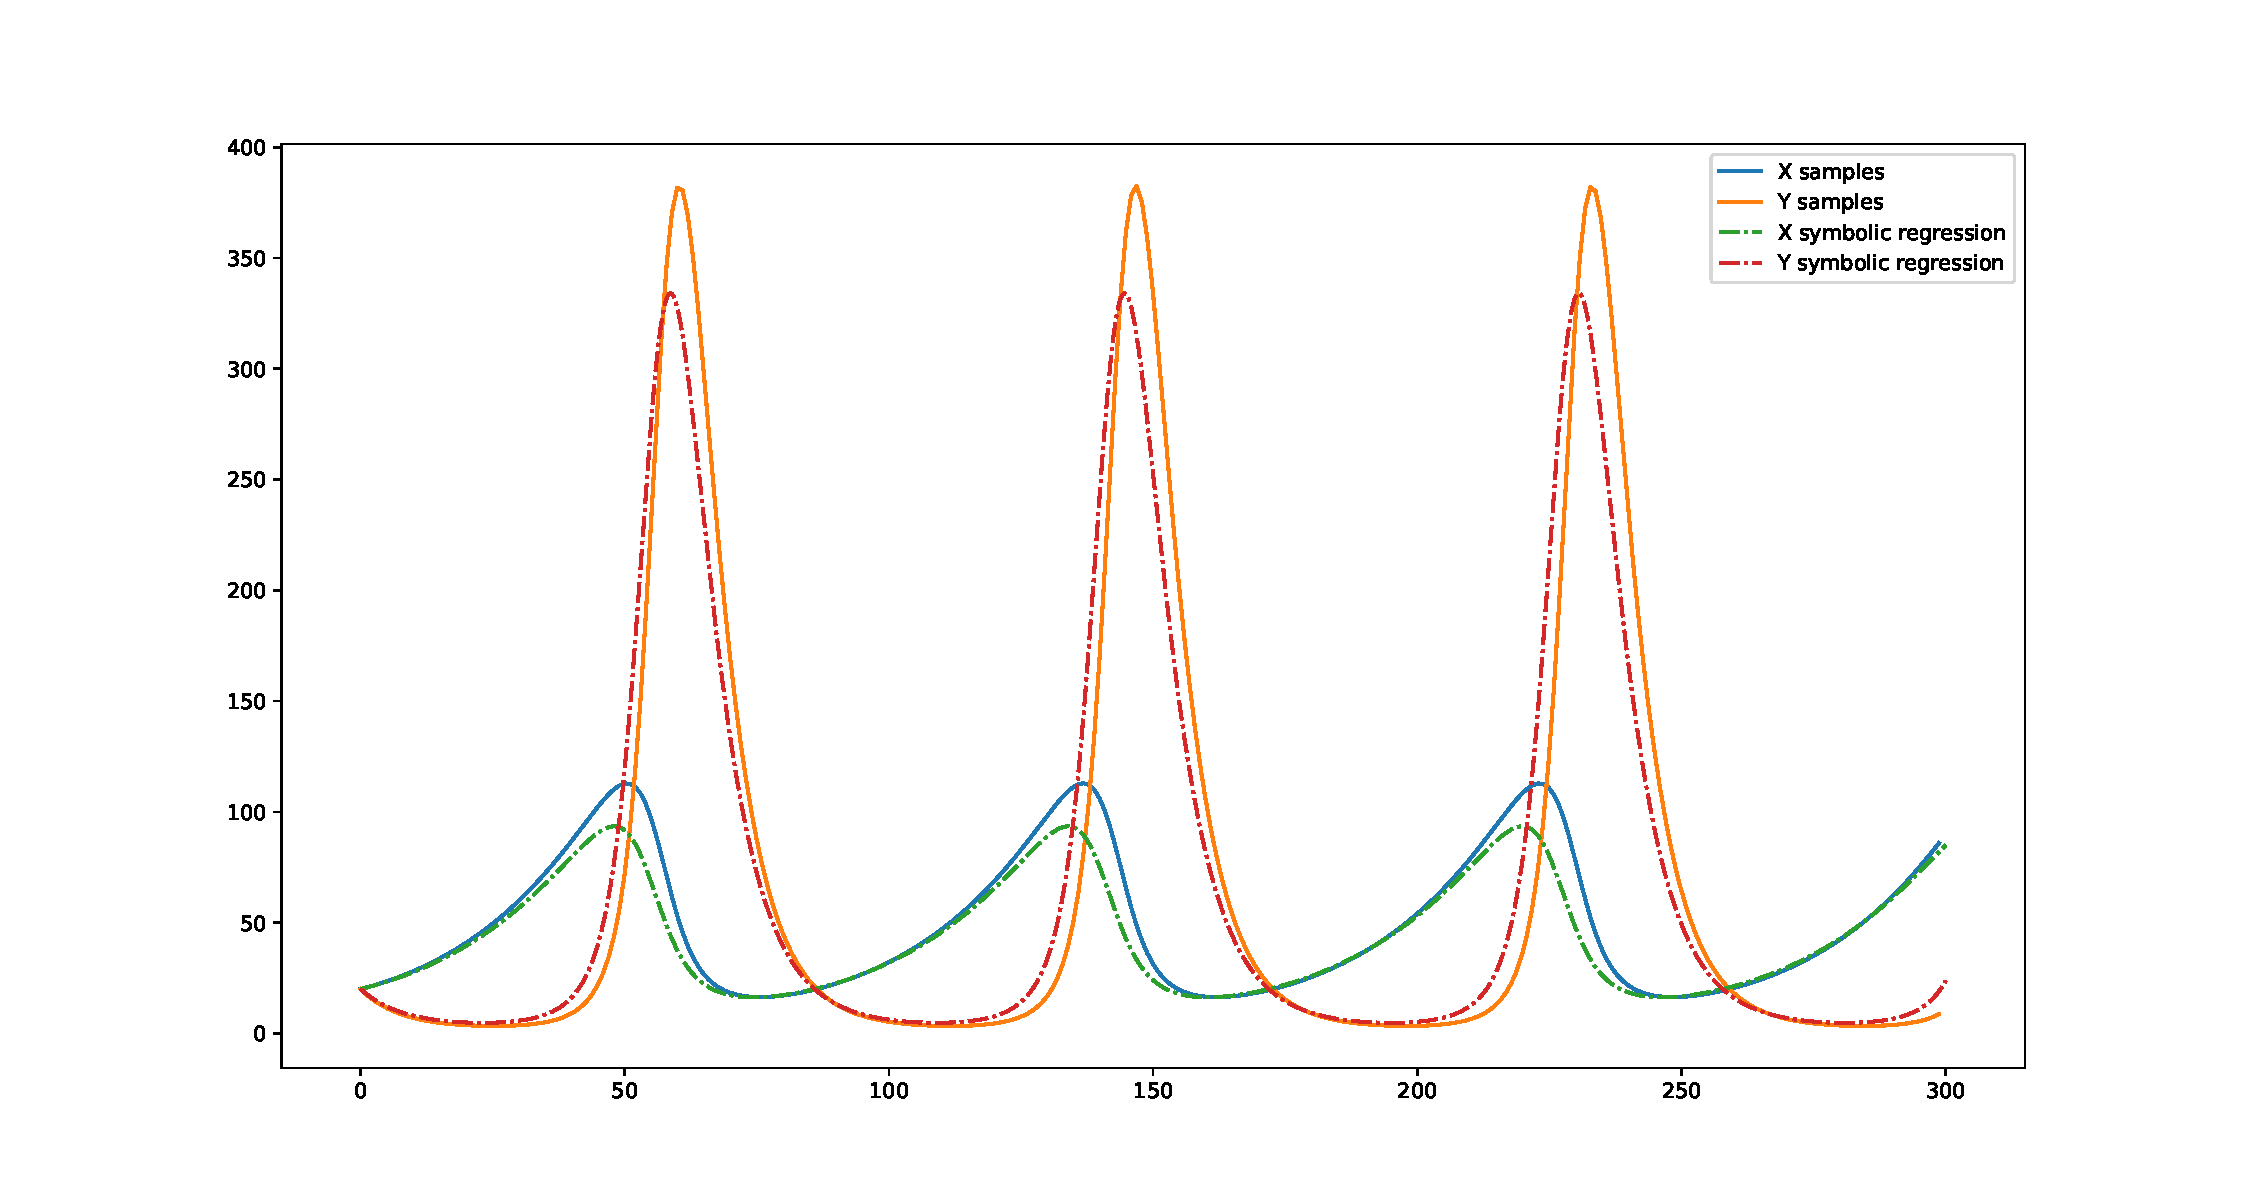
\includegraphics[width=\textwidth]{"figures/final_plot_LV_0.0.pdf"}
    \caption{Modelo resultante utilizando datos generados a partir del modelo lotka-volterra con ruido máximo de 0\%.}
    \label{fig:final_plot_LV_0.0}
\end{figure}

\begin{figure}[h]
    \centering
    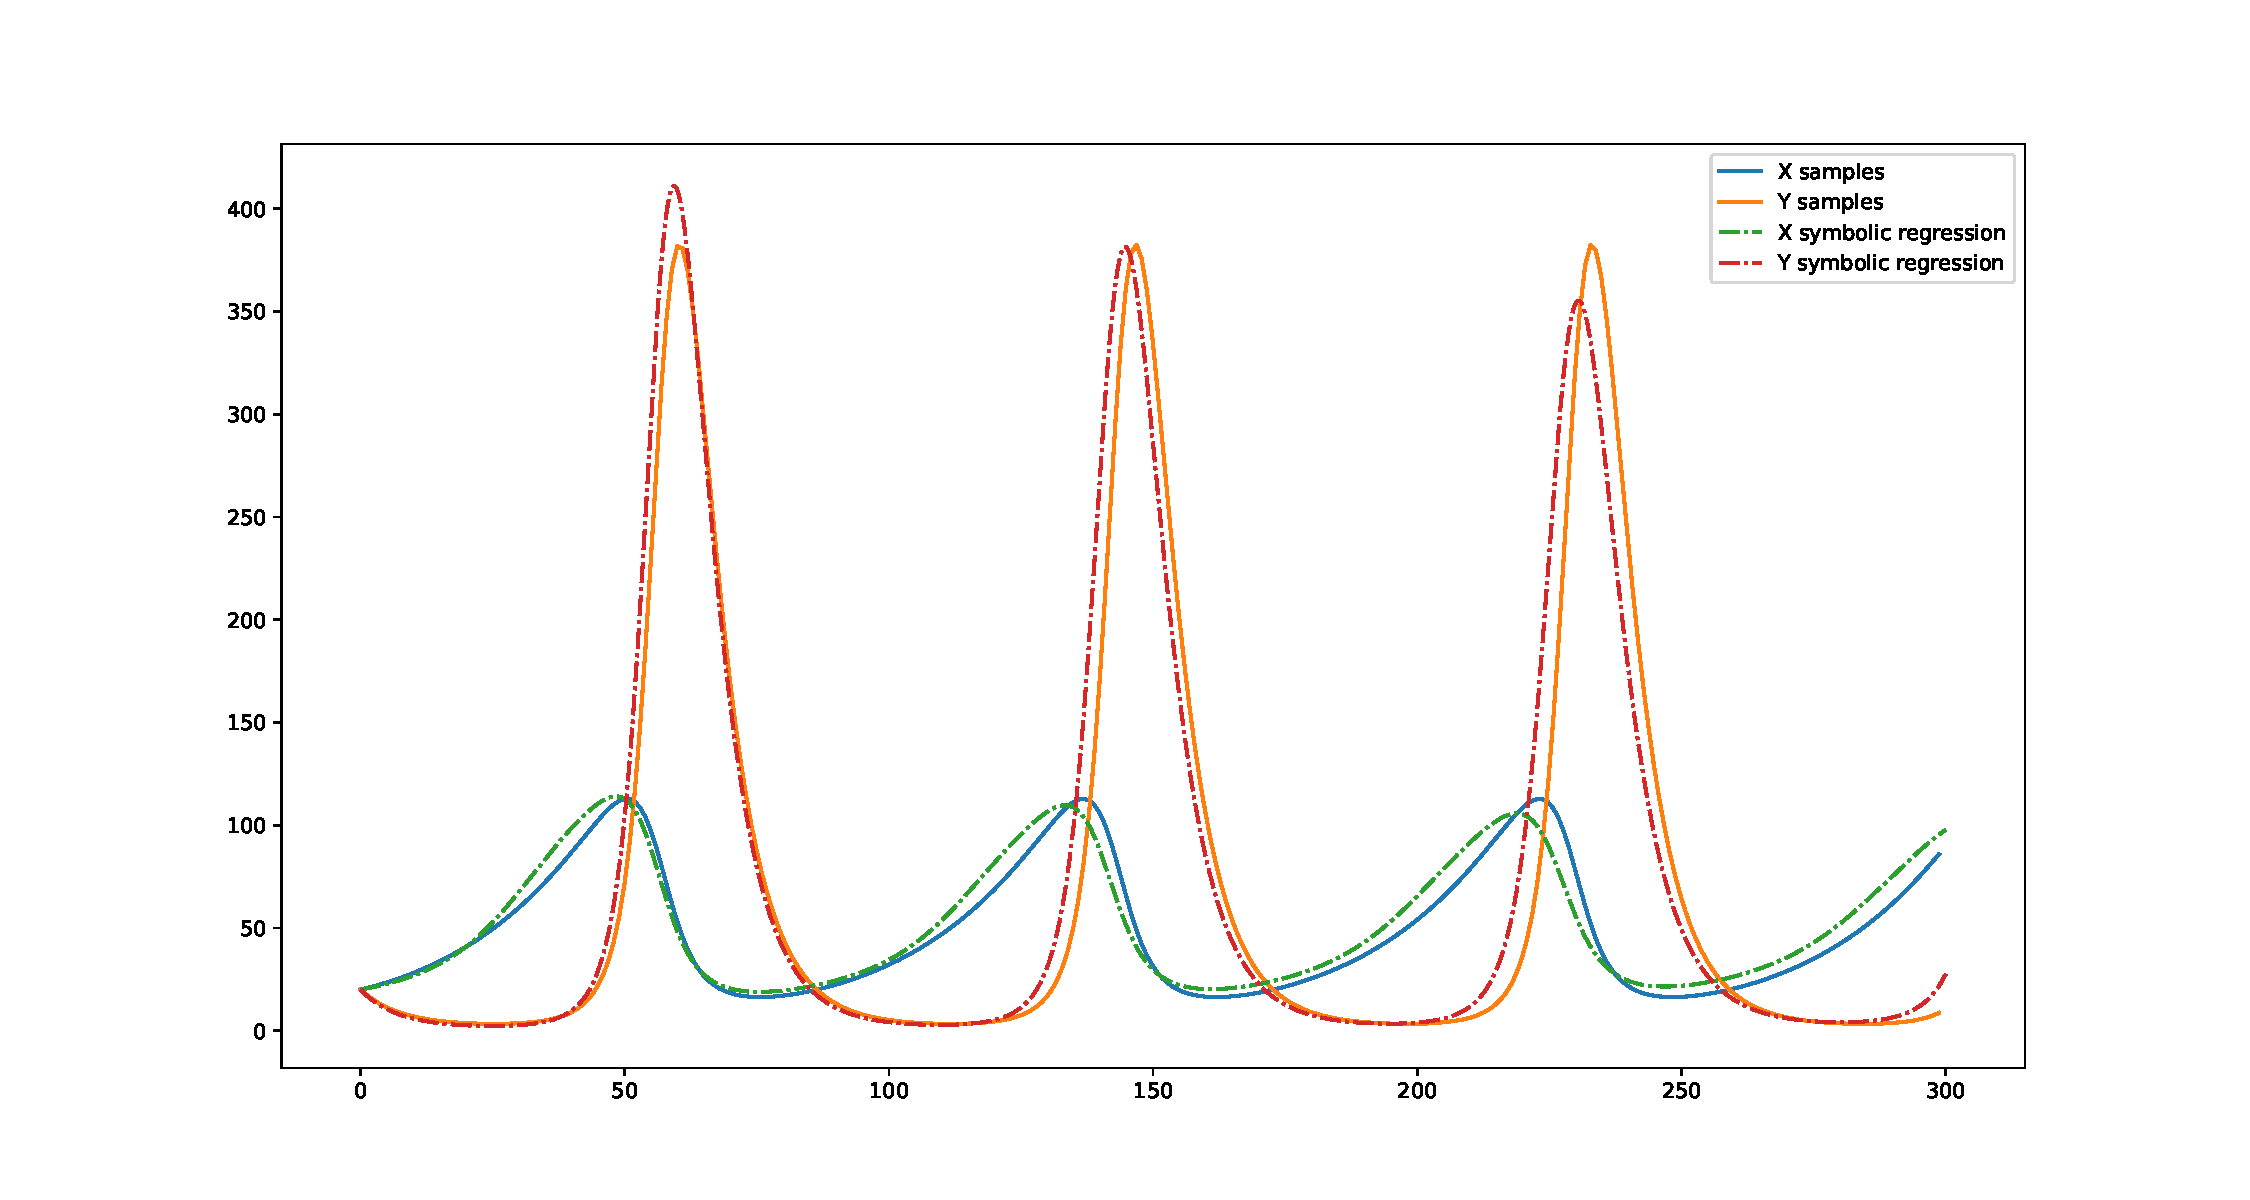
\includegraphics[width=\textwidth]{"figures/final_plot_LV_0.05.pdf"}
    \caption{Modelo resultante utilizando datos generados a partir del modelo lotka-volterra con ruido máximo de 5\%.}
    \label{fig:final_plot_LV_0.05}
\end{figure}

\begin{figure}[h]
    \centering
    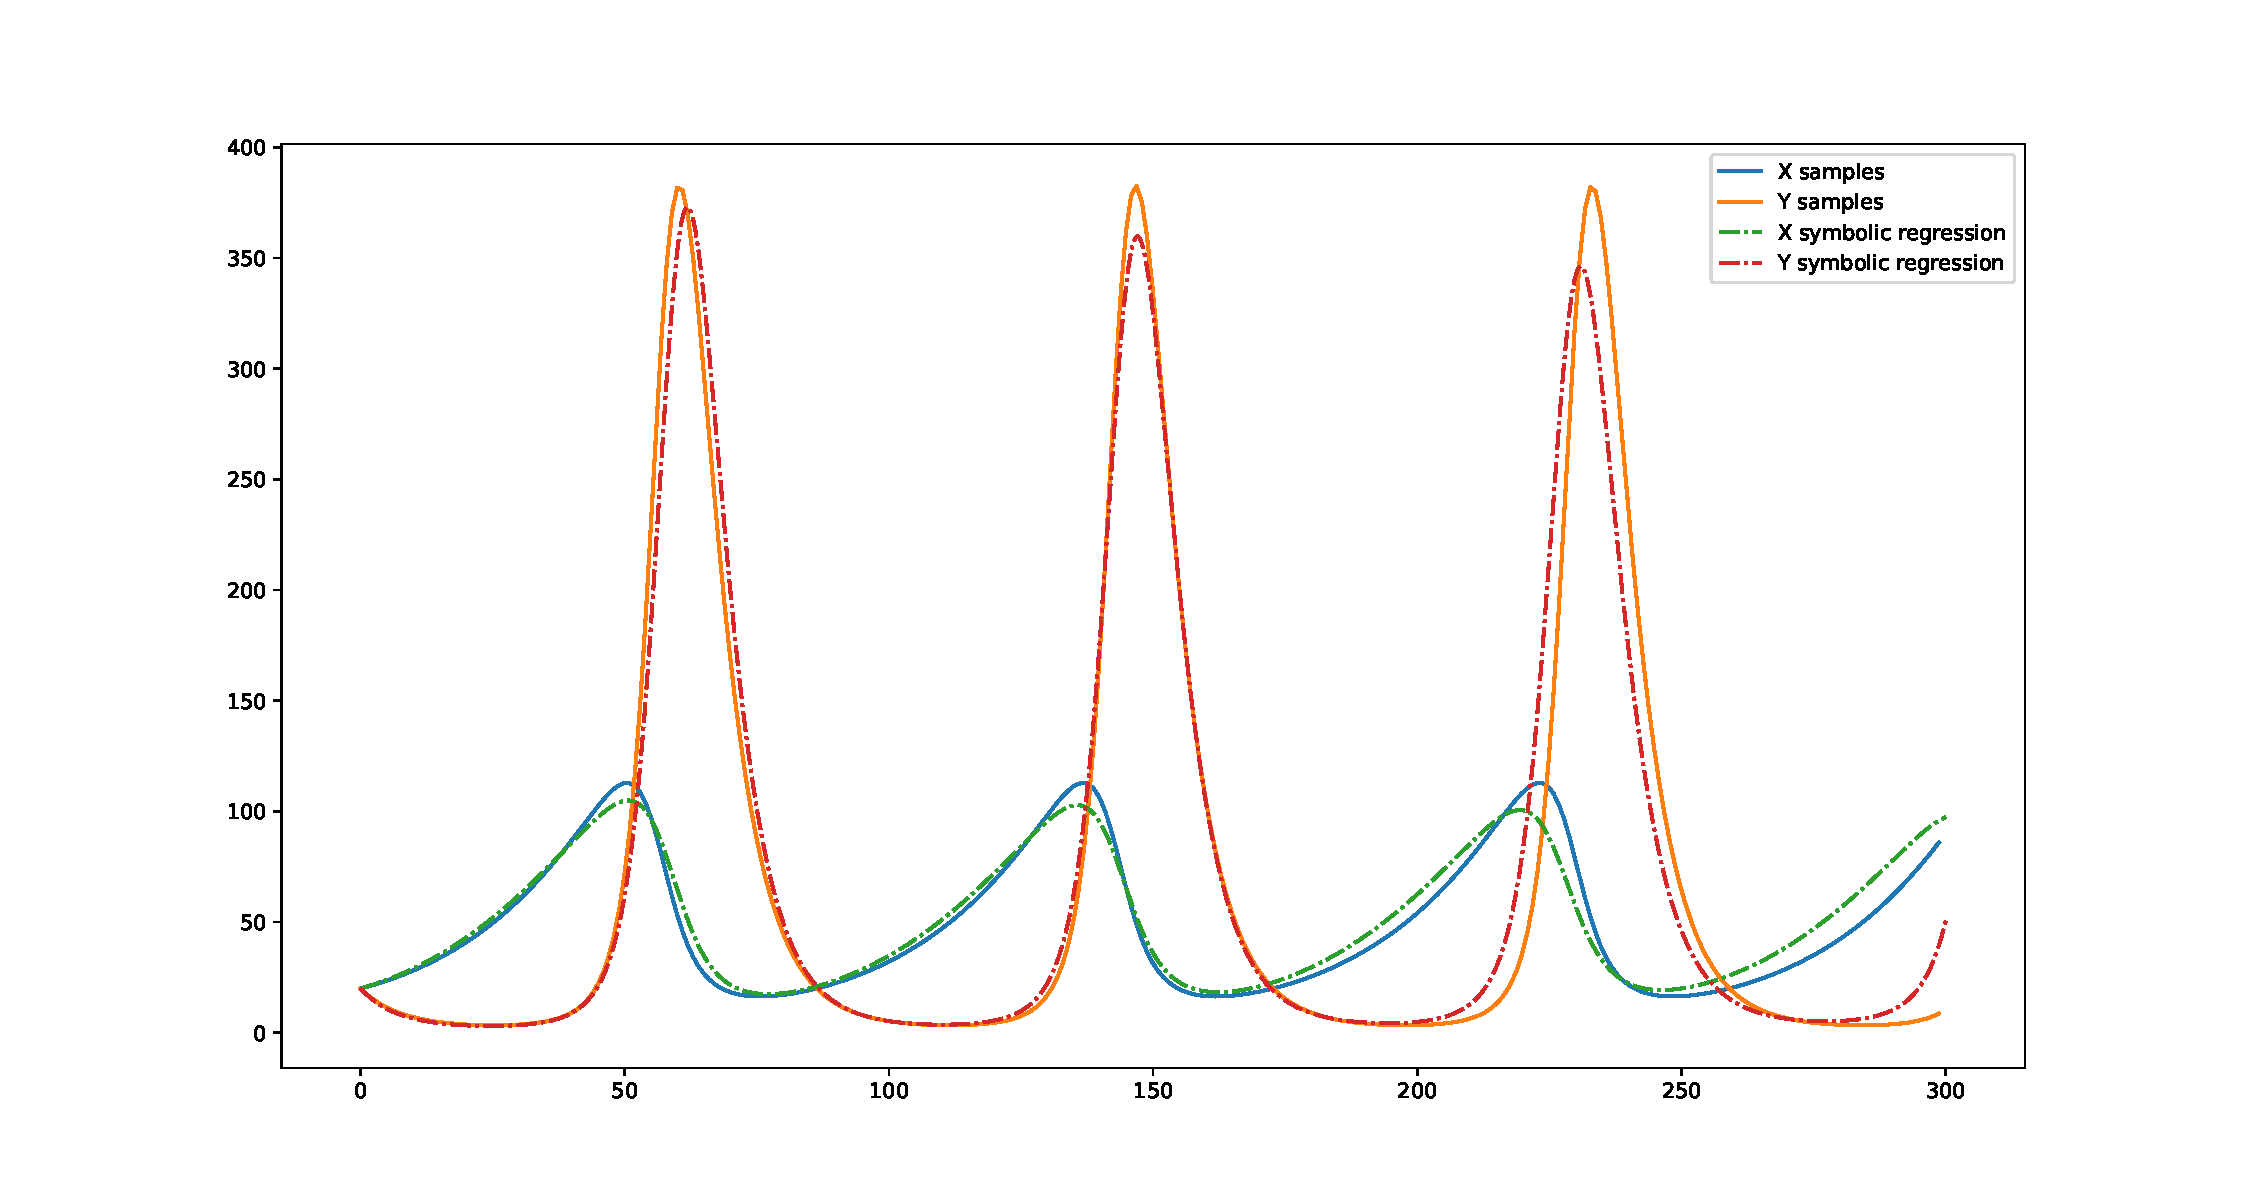
\includegraphics[width=\textwidth]{"figures/final_plot_LV_0.1.pdf"}
    \caption{Modelo resultante utilizando datos generados a partir del modelo lotka-volterra con ruido máximo de 10\%.}
    \label{fig:final_plot_LV_0.1}
\end{figure}


En el resto de experimentos realizados utilizando otros modelos, nunca se obtuvo como resultado de la regresión simbólica el modelo original que generó los datos.

Si en lugar de utilizar como aproximación el método de diferencias finitas cuando los datos no poseen ruido, se utiliza el sistema original de Lotka-Volterra, se obtiene que la media del valor de la función de ajuste a lo largo de las 30 ejecuciones del experimento es $0.00721$. El valor máximo de la función de ajuste alcanzado fue de $0.21654$ y el mínimo de $6.35015e-16$, en este último la regresión simbólica obtuvo exactamente el sistema utilizado para generar los datos.


A continuación se muestra el experimento realizado a partir de la generación de los datos utilizando el sistema SIR.

\subsection{SIR}

El modelo SIR es un sistema que se utiliza para describir la transmición de una enfermedad infecciosa causada por una bacteria, virus u hongos. \cite{weiss2013sir}. El sistema se define como:

\begin{align*}
    S' & = - aIS    \\
    I' & = aIS - bI \\
    R' & = bI,
\end{align*}

donde $S$ indica la cantidad de personas susceptibles, $I$ la cantidad de personas infectadas y $R$ la cantidad de personas recuperadas. Se utiliza el parámetro $a$ para indicar el índice de transmición y $b$ el índice de recuperación de la enfermedad.

Se utilizaron como valores de los parámetros $a = 0.0003$ y $b = 0.1$ con punto inicial $(700, 300, 0)$ y se integró en el intervalo $0 \leq t \leq 20$ para obtener los datos que aparecen en la imagen \ref{fig:SIR} de la página \pageref{fig:SIR}. Del conjunto de puntos se seleccionaron 300 muestras como datos para el método de regresión simbólica.

Los resultados que se obtienen durante las 30 ejecuciones del experimento, utilizando solamente en cada ecuación las variables permitidas según el modelo, aparecen en la tabla \ref{table:experiment_SIR} de la página \pageref{table:experiment_SIR}. Si se permite cualquier variable del modelo en cualquier ecuación del sistema se obtienen los datos que aparecen en la tabla \ref{table:experiment_SIR_all} de la página \pageref{table:experiment_SIR_all}.

\begin{table}[!h]
    \centering
    \caption{Resultados que se obtienen en el modelo SIR restringiendo las variables que aparecen en cada ecuación.}
    \begin{tabular}{|c|c|c|c|}
        \hline
               & \textbf{ruido de 0\%} & \textbf{ruido de 5\%} & \textbf{ruido de 10\%} \\
        \hline
        media  & 0.25506               & 4.78621               & 6.9987                 \\
        \hline
        mínimo & 0.2187                & 0.79521               & 1.48455                \\
        \hline
        máximo & 0.30485               & 31.77664              & 51.66934               \\
        \hline
    \end{tabular}

    \begin{tabular}{|c|c|c|c|c|c|}
        \hline
                             & \textbf{ruido de 0\%} & \textbf{ruido de 5\%} & \textbf{ruido de 10\%} \\
        \hline
        cantidad de sistemas & 30                    & 28                    & 28                     \\
        \hline
        original             & 2.02689               & 60.79755              & 117.71809              \\
        \hline
        original con ruido   & 2.02689               & 66.59004              & 130.68564              \\
        \hline
        spline               & 2.02689               & 61.046                & 117.83595              \\
        \hline
        otro método          & 31160.12619           & 27363.87727           & 35775.36901            \\
        \hline
    \end{tabular}
    \label{table:experiment_SIR}
\end{table}

\begin{table}[!h]
    \centering
    \caption{Resultados que se obtienen en el modelo SIR sin restringir las variables que aparecen en cada ecuación.}
    \begin{tabular}{|c|c|c|c|}
        \hline
               & \textbf{ruido de 0\%} & \textbf{ruido de 5\%} & \textbf{ruido de 10\%} \\
        \hline
        media  & 0.24689               & 3.42671               & 5.1537                 \\
        \hline
        mínimo & 0.05612               & 0.7473                & 1.4416                 \\
        \hline
        máximo & 0.43011               & 13.57073              & 50.52157               \\
        \hline
    \end{tabular}

    \begin{tabular}{|c|c|c|c|c|c|}
        \hline
                             & \textbf{ruido de 0\%} & \textbf{ruido de 5\%} & \textbf{ruido de 10\%} \\
        \hline
        cantidad de sistemas & 30                    & 30                    & 26                     \\
        \hline
        original             & 1.79636               & 69.15052              & 42.3377                \\
        \hline
        original con ruido   & 1.79636               & 76.12959              & 58.03488               \\
        \hline
        spline               & 1.79636               & 69.23198              & 42.15867               \\
        \hline
        otro método          & 31160.16998           & 27425.68474           & 35588.9792             \\
        \hline
    \end{tabular}
    \label{table:experiment_SIR_all}
\end{table}

Durante la realización de los experimentos utilizando el modelo SIR nunca se obtuvo un sistema igual como resultado de la regresión simbólica. Pero el resultado ajustó los datos no importa la cantidad de ruido utilizado. Los datos que se obtienen de la integración del sistema resultante de la regresión simbólica se asemejan a los datos de la integración del sistema seleccionado para la realización del experimento pero la aparición de ruido afecta el ajuste de los datos.

En las figuras \ref{fig:final_plot_SIR_0.0} de la página \pageref{fig:final_plot_SIR_0.0}, \ref{fig:final_plot_SIR_0.05} de la página \pageref{fig:final_plot_SIR_0.05} y \ref{fig:final_plot_SIR_0.1} de la página \pageref{fig:final_plot_SIR_0.1} se pueden ver los datos originales comparados con los datos obtenidos del mejor resultado generado por la regresión simbólica restringiendo las variables que pueden existir en cada ecuación.

\begin{figure}[h]
    \centering
    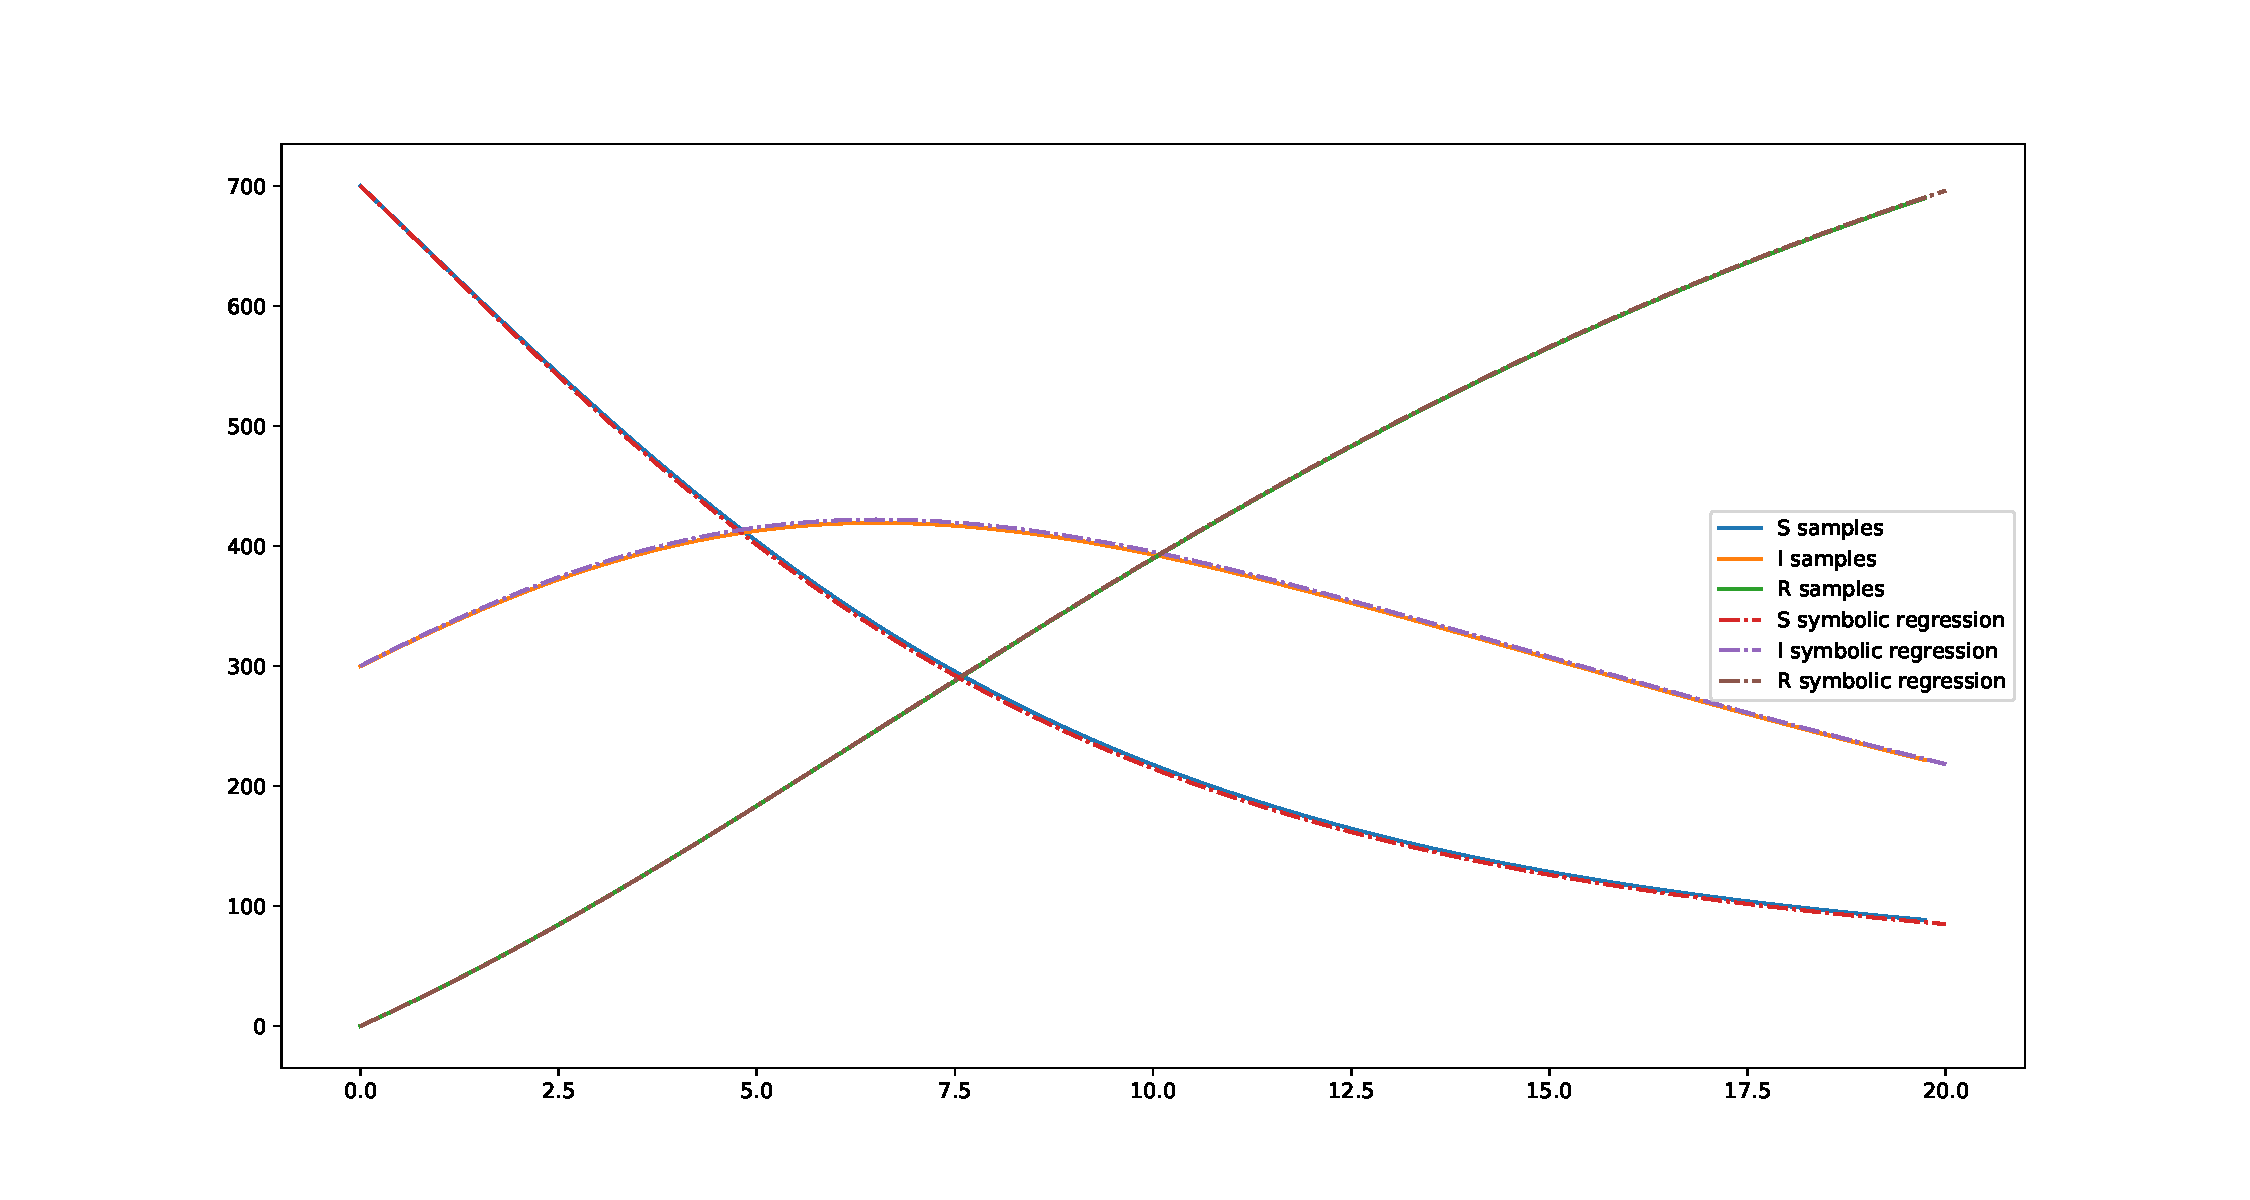
\includegraphics[width=\textwidth]{"figures/final_plot_SIR_0.0.pdf"}
    \caption{Modelo resultante utilizando datos generados a partir del modelo SIR con ruido máximo de 0\%.}
    \label{fig:final_plot_SIR_0.0}
\end{figure}

\begin{figure}[h]
    \centering
    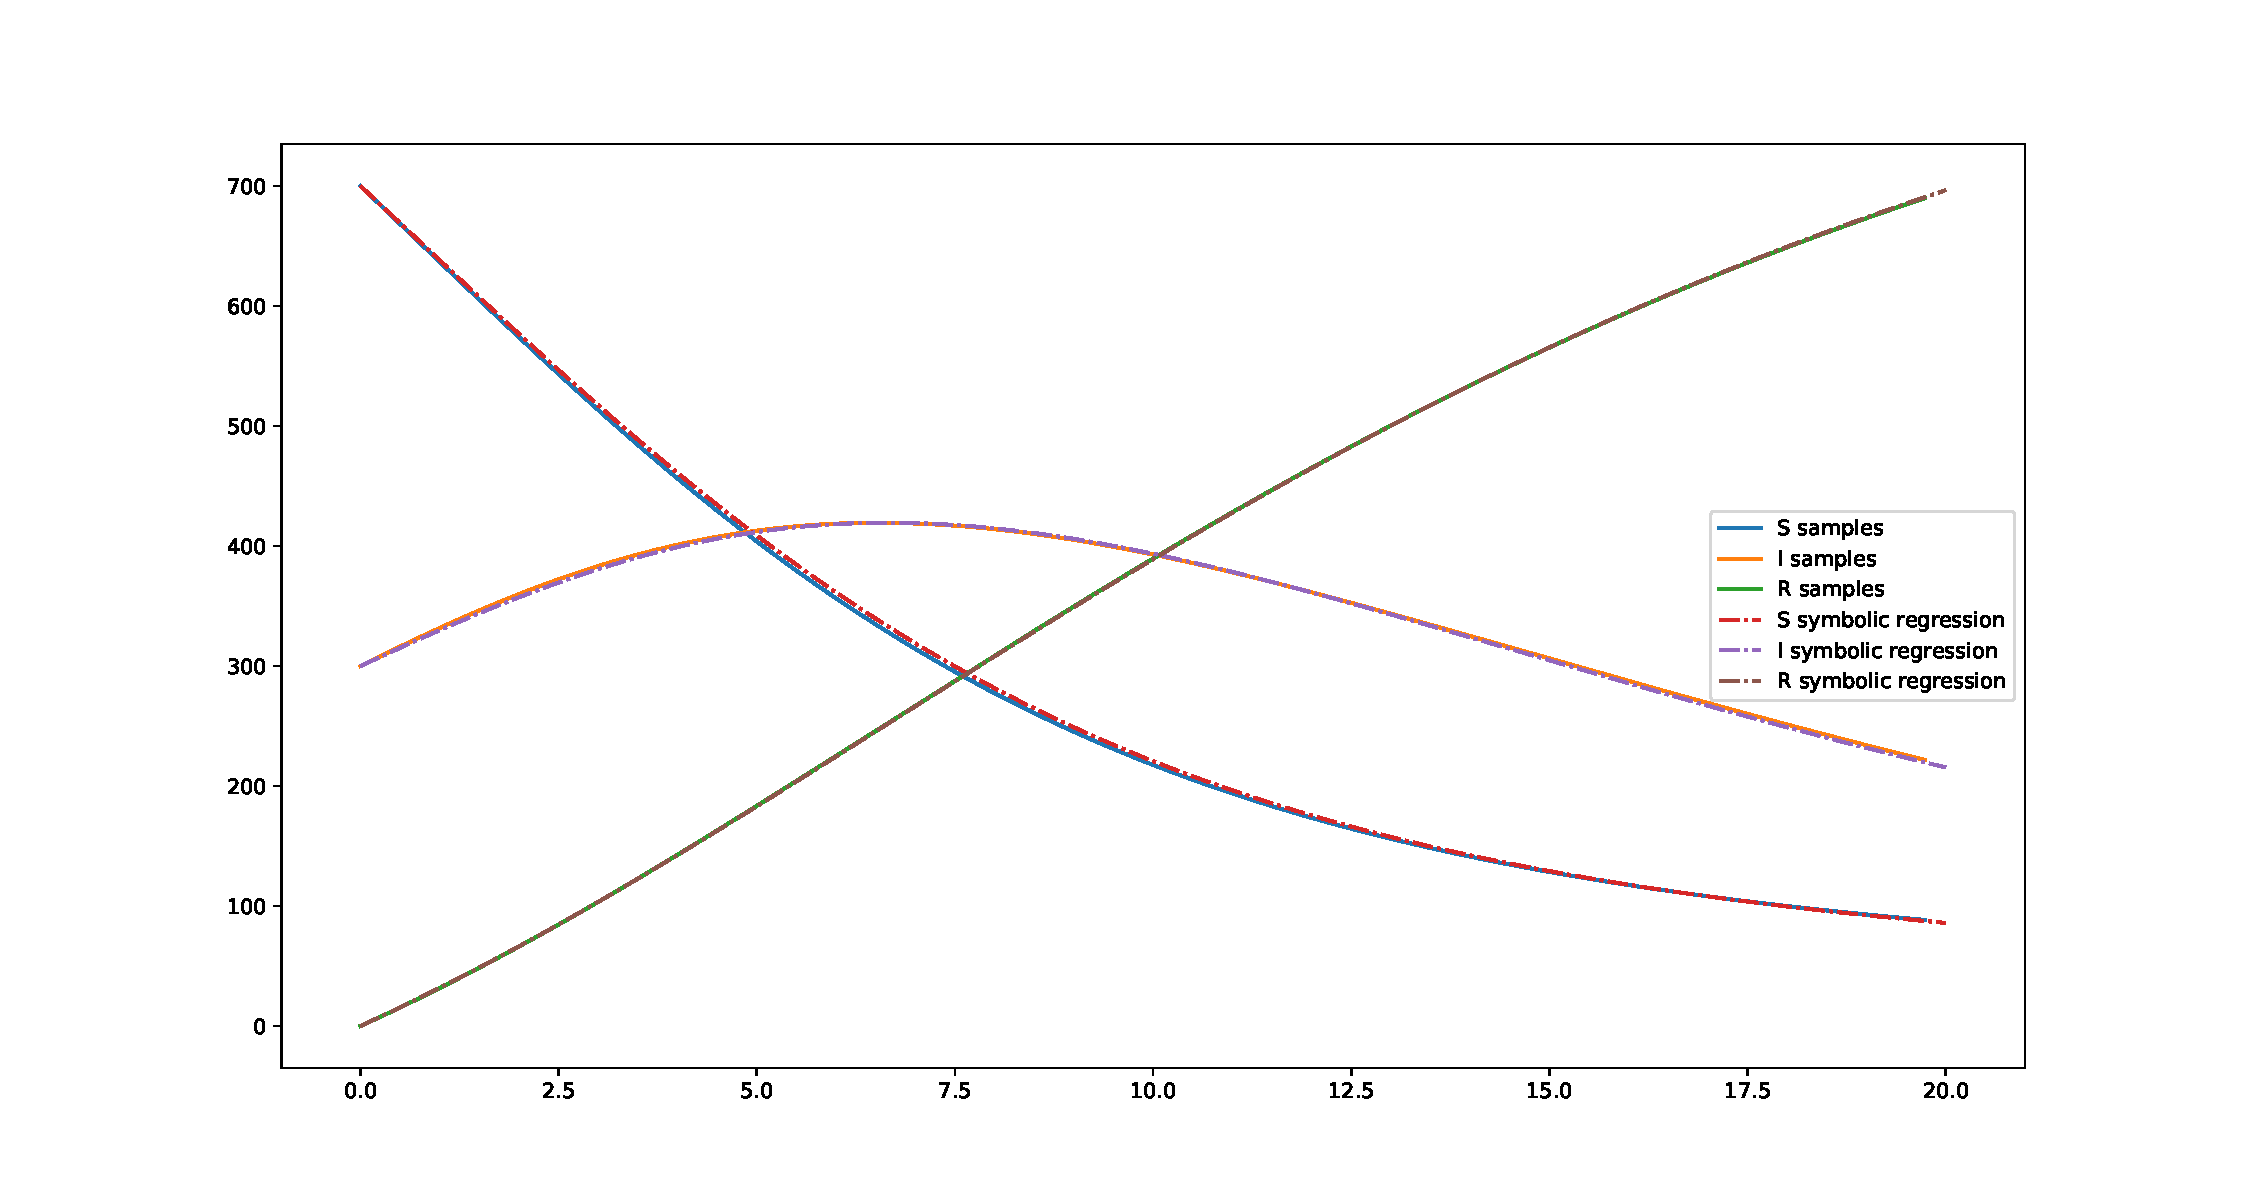
\includegraphics[width=\textwidth]{"figures/final_plot_SIR_0.05.pdf"}
    \caption{Modelo resultante utilizando datos generados a partir del modelo SIR con ruido máximo de 5\%.}
    \label{fig:final_plot_SIR_0.05}
\end{figure}

\begin{figure}[h]
    \centering
    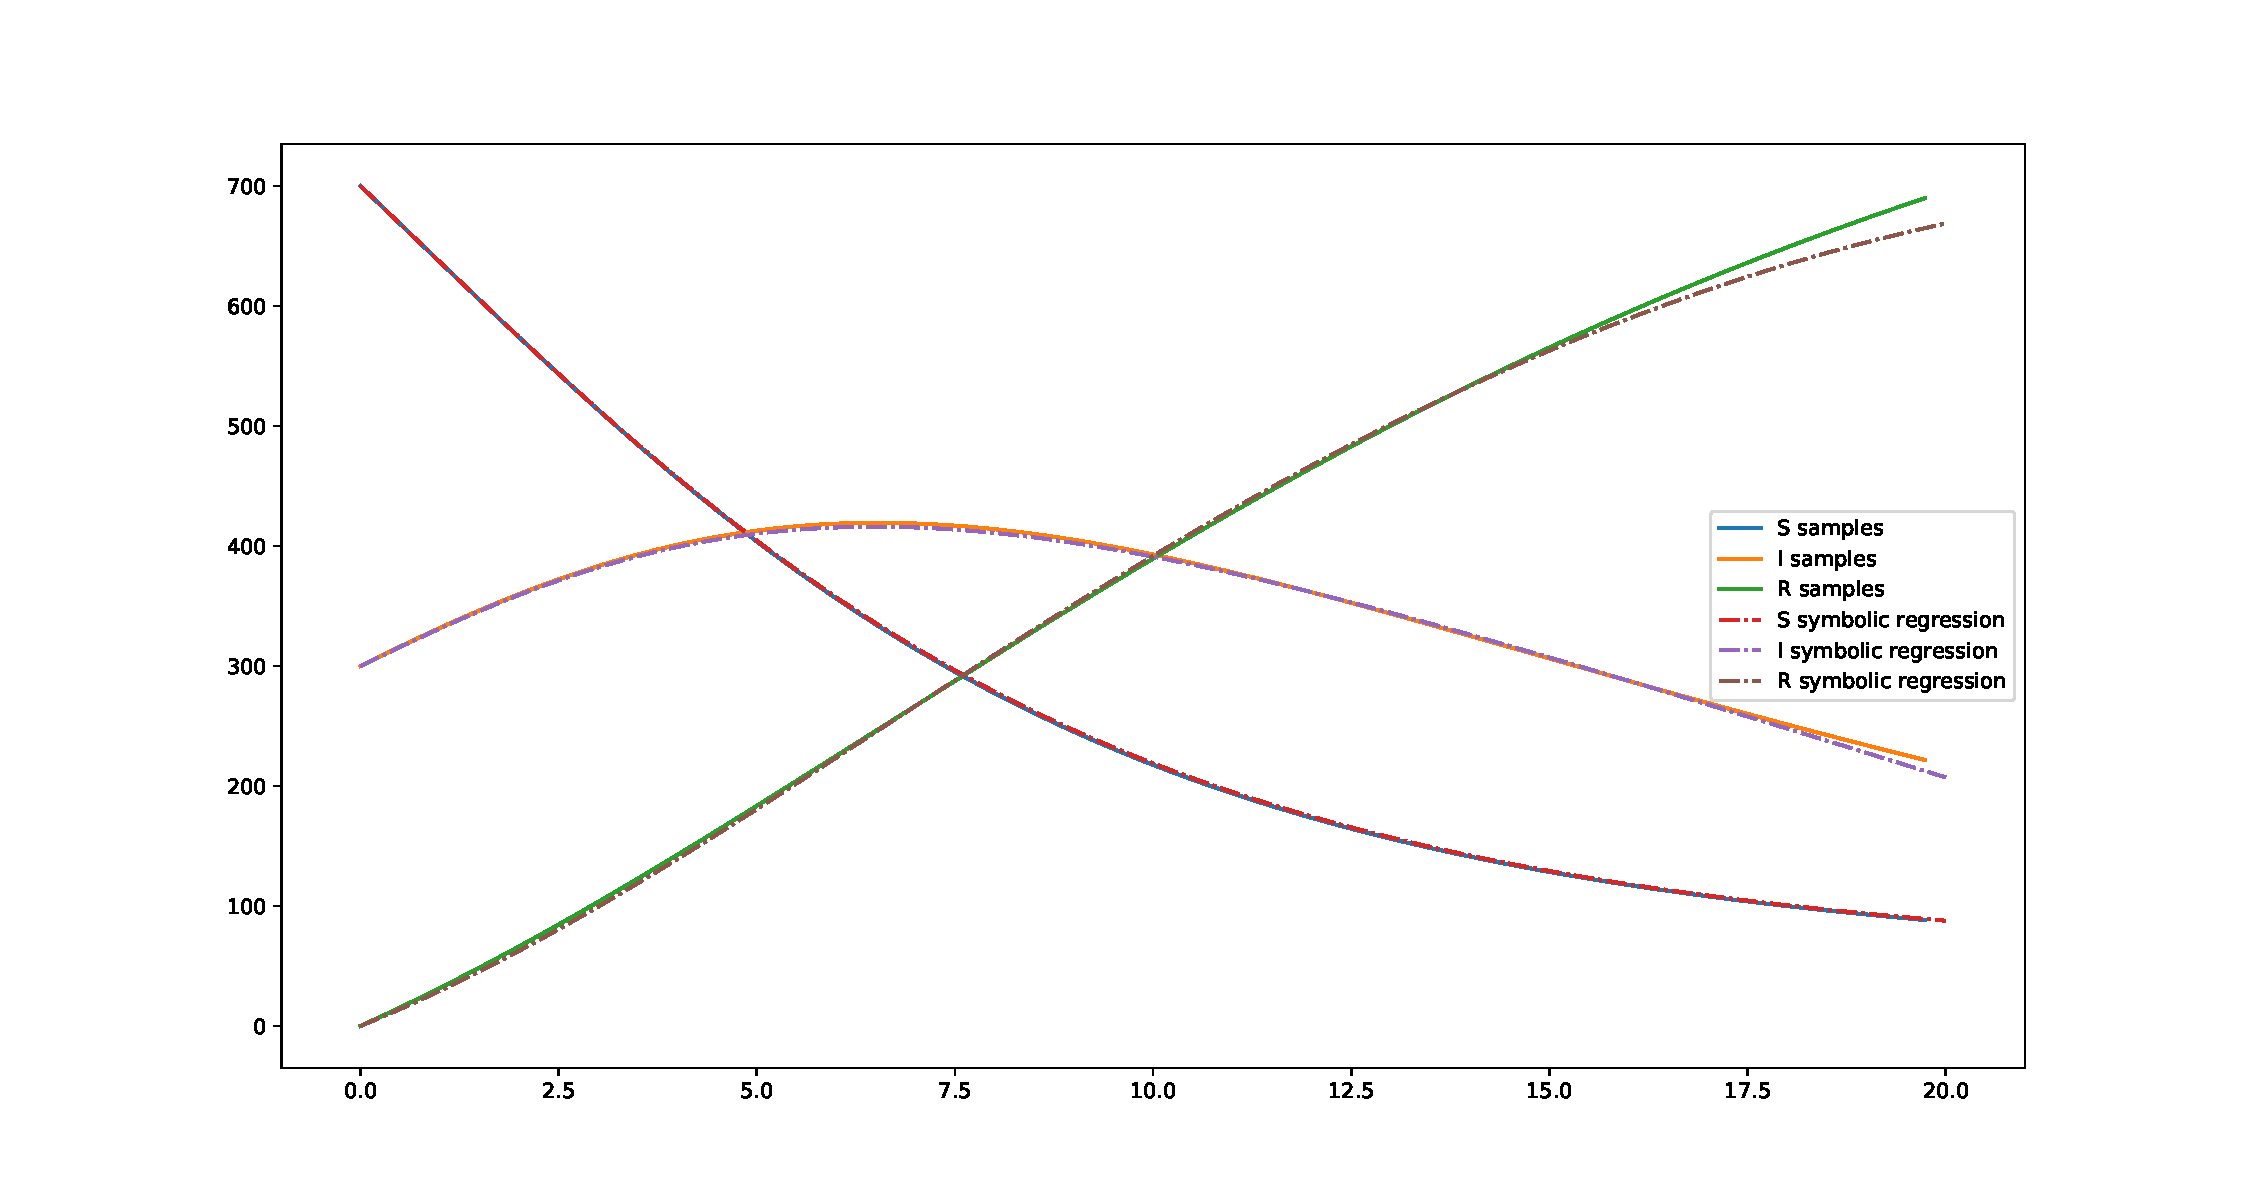
\includegraphics[width=\textwidth]{"figures/final_plot_SIR_0.1.pdf"}
    \caption{Modelo resultante utilizando datos generados a partir del modelo SIR con ruido máximo de 10\%.}
    \label{fig:final_plot_SIR_0.1}
\end{figure}

Si en lugar de utilizar como aproximación el método de diferencias finitas cuando los datos no poseen ruido, se utiliza el sistema original de SIR, se obtiene que la media del valor de la función de ajuste a lo largo de las 30 ejecuciones del experimento es $7.02137e-05$. El valor máximo de la función de ajuste alcanzado fue de $ 0.00116$ y el mínimo de $1.19509e-15$, en este último la regresión simbólica obtuvo exactamente el sistema utilizado para generar los datos.

A continuación se muestra el experimento realizado a partir de la generación de datos utilizando el sistema SIRD.

\subsection{SIRD}

El modelo SIRD es un sistema similar al SIR pero que introduce como dato la cantidad de personas fallecidas $D$ \cite{bailey1975mathematical}. Al modelo SIRD mencionado en \cite{bailey1975mathematical} se le realizó una modificación al añadir un parámetro representando la cantidad de personas que pasan a ser susceptibles en cada instante de tiempo. El sistema se define como:

\begin{align*}
    S' & = a - b (\frac{S I}{S + I + R})         \\
    I' & = b (\frac{S I}{S + I + R}) - c I - d I \\
    R' & = c I                                   \\
    D' & = d I,
\end{align*}

donde $a$ representa la cantidad de personas que pasan a ser susceptibles, $b$ es el índice de contagio de la enfermedad, $c$ es el índice de recuperación y $d$ es el índice de muerte a causa de la enfermedad.

Se utilizaron como valores de los parámetros $a = 250$, $b = 0.5$, $c = 0.1$ y $d = 0.2$ con punto inicial $(7000, 3000, 0, 0)$ y se integró en el intervalo $0 \leq t \leq 20$ para obtener los datos que aparecen en la figura \ref{fig:SIRD}. Del conjunto de puntos se seleccionaron 300 muestras como datos para el método de regresión simbólica.

\begin{figure}[h]
    \centering
    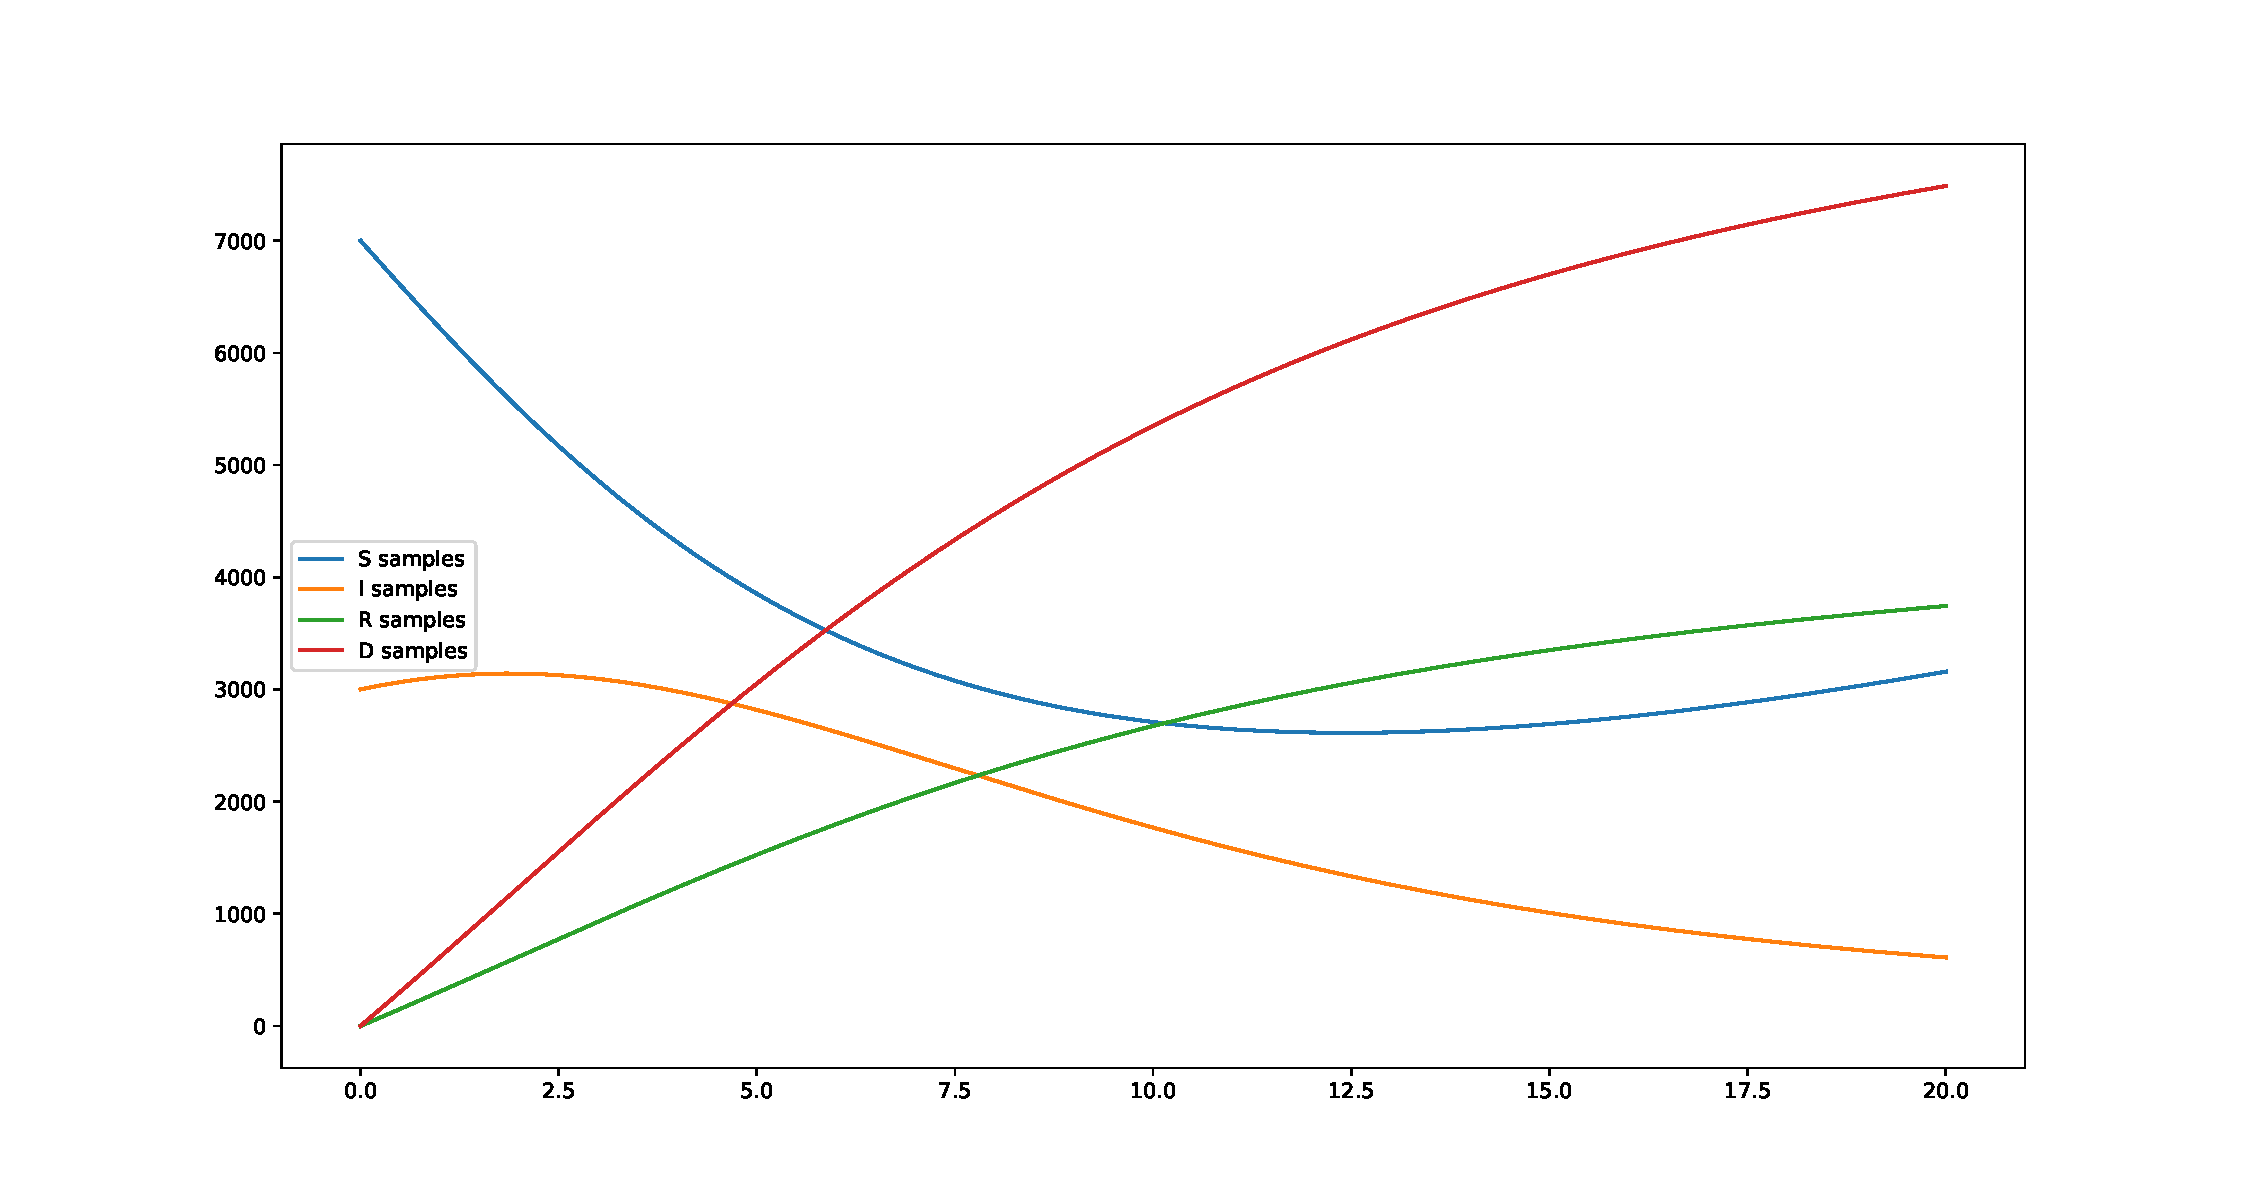
\includegraphics[width=\textwidth]{"figures/SIRD.pdf"}
    \caption{modelo SIRD con $a = 250$, $b = 0.5$, $c = 0.1$ y $d = 0.2$.}
    \label{fig:SIRD}
\end{figure}

Los resultados que se obtienen durante las 30 ejecuciones del experimento, utilizando solamente en cada ecuación las variables permitidas según el modelo y además se agrega como varible $N=S + I + R$, aparecen en la tabla \ref{table:experiment_SIRD} de la página \pageref{table:experiment_SIRD}. Si se permite cualquier variable del modelo en cualquier ecuación del sistema se obtienen los datos que aparecen en la tabla \ref{table:experiment_SIRD_all} de la página \pageref{table:experiment_SIRD_all}.

\begin{table}[!h]
    \centering
    \caption{Resultados que se obtienen en el modelo SIRD restringiendo las variables que aparecen en cada ecuación.}
    \begin{tabular}{|c|c|c|c|}
        \hline
               & \textbf{ruido de 0\%} & \textbf{ruido de 5\%} & \textbf{ruido de 10\%} \\
        \hline
        media  & 47.66074              & 90.64233              & 244.82477              \\
        \hline
        mínimo & 0.51207               & 10.05468              & 18.63161               \\
        \hline
        máximo & 133.55556             & 569.35212             & 2450.05618             \\
        \hline
    \end{tabular}

    \begin{tabular}{|c|c|c|c|c|c|}
        \hline
                             & \textbf{ruido de 0\%} & \textbf{ruido de 5\%} & \textbf{ruido de 10\%} \\
        \hline
        cantidad de sistemas & 22                    & 20                    & 21                     \\
        \hline
        original             & 520.90815             & 894.24332             & 851.17623              \\
        \hline
        original con ruido   & 520.90815             & 917.42578             & 910.64791              \\
        \hline
        spline               & 520.90815             & 894.29561             & 848.03264              \\
        \hline
        otro método          & 596.93643             & 631.63455             & 735.58784              \\
        \hline
    \end{tabular}
    \label{table:experiment_SIRD}
\end{table}

\begin{table}[!h]
    \centering
    \caption{Resultados que se obtienen en el modelo SIRD sin restringir las variables que aparecen en cada ecuación.}
    \begin{tabular}{|c|c|c|c|}
        \hline
               & \textbf{ruido de 0\%} & \textbf{ruido de 5\%} & \textbf{ruido de 10\%} \\
        \hline
        media  & 18.06453              & 109.07249             & 40.10858               \\
        \hline
        mínimo & 0.86131               & 10.14889              & 13.82246               \\
        \hline
        máximo & 49.33228              & 2116.3281             & 193.21428              \\
        \hline
    \end{tabular}

    \begin{tabular}{|c|c|c|c|c|c|}
        \hline
                             & \textbf{ruido de 0\%} & \textbf{ruido de 5\%} & \textbf{ruido de 10\%} \\
        \hline
        cantidad de sistemas & 27                    & 26                    & 24                     \\
        \hline
        original             & 248.31329             & 579.93813             & 652.00833              \\
        \hline
        original con ruido   & 248.31329             & 616.80845             & 743.63415              \\
        \hline
        spline               & 248.31329             & 579.74029             & 644.37875              \\
        \hline
        otro método          & 672.43116             & 674.83326             & 504.66352              \\
        \hline
    \end{tabular}
    \label{table:experiment_SIRD_all}
\end{table}

Durante la realización de los experimentos utilizando el modelo SIRD nunca se obtuvo un sistema igual como resultado de la regresión simbólica, además no se ajustan los datos no importa la cantidad de ruido. El sistema SIRD que se utiliza es el único sistema entre todos los experimentos que posee un término en una ecuación donde aparece un parámetro sin una expresión que lo acompañe.

Los datos que se obtienen de la integración del sistema resultante de la regresión simbólica no se asemejan a los datos de la integración del sistema seleccionado para la realización del experimento, la aparición de ruido afecta aún más el ajuste de los datos.

En las figuras \ref{fig:final_plot_SIRD_0.0} de la página \pageref{fig:final_plot_SIRD_0.0}, \ref{fig:final_plot_SIRD_0.05} de la página \pageref{fig:final_plot_SIRD_0.05} y \ref{fig:final_plot_SIRD_0.1} de la página \pageref{fig:final_plot_SIRD_0.1} se pueden ver los datos originales comparados con los datos obtenidos del mejor resultado generado por la regresión simbólica restringiendo las variables que pueden existir en cada ecuación.

\begin{figure}[h]
    \centering
    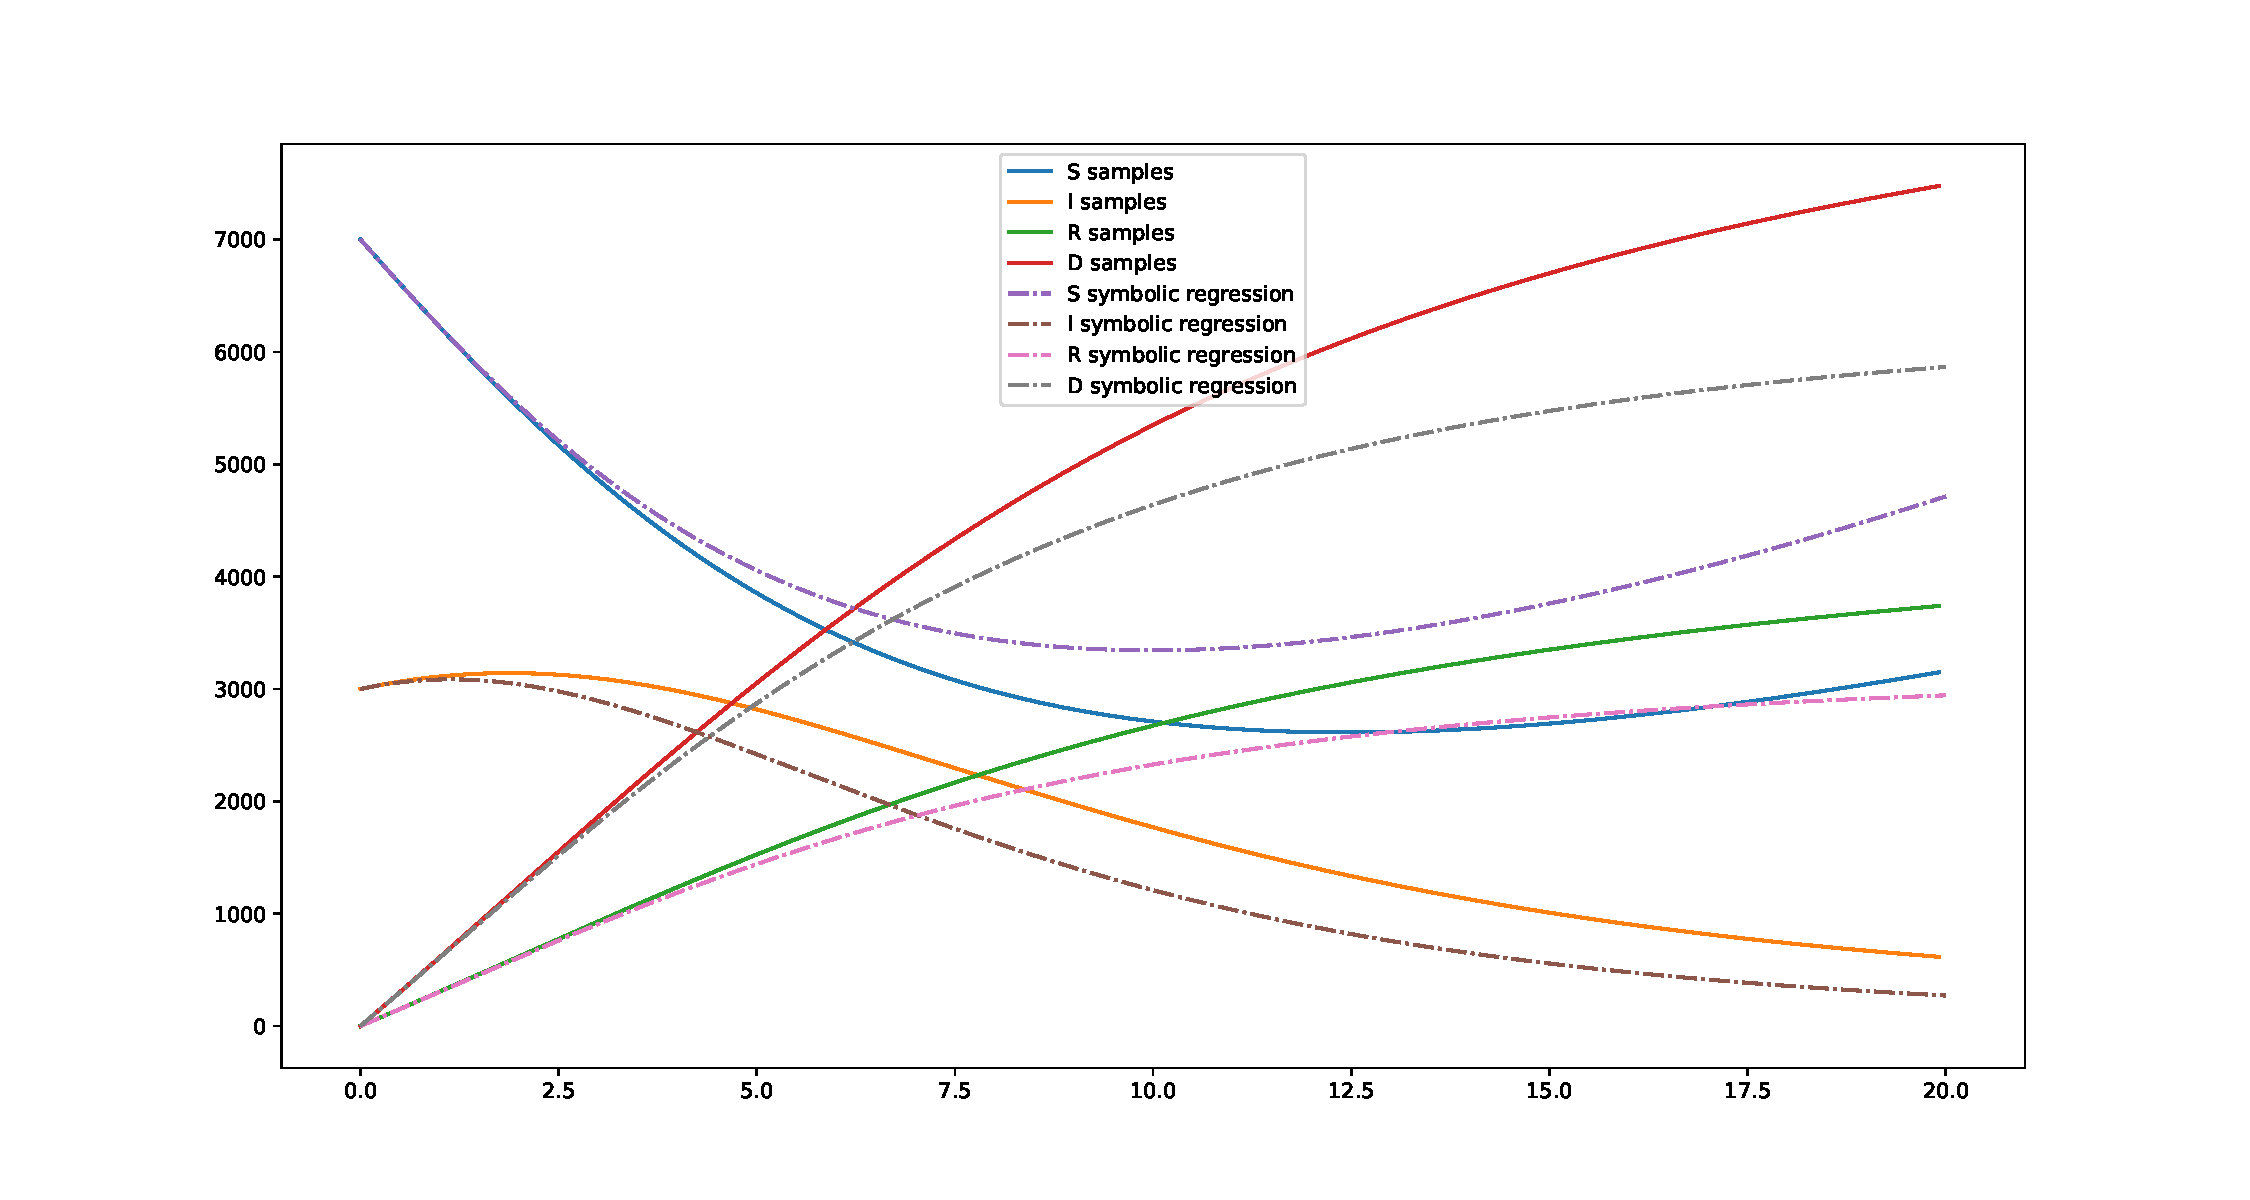
\includegraphics[width=\textwidth]{"figures/final_plot_SIRD_0.0.pdf"}
    \caption{Modelo resultante utilizando datos generados a partir del modelo SIRD con ruido máximo de 0\%.}
    \label{fig:final_plot_SIRD_0.0}
\end{figure}

\begin{figure}[h]
    \centering
    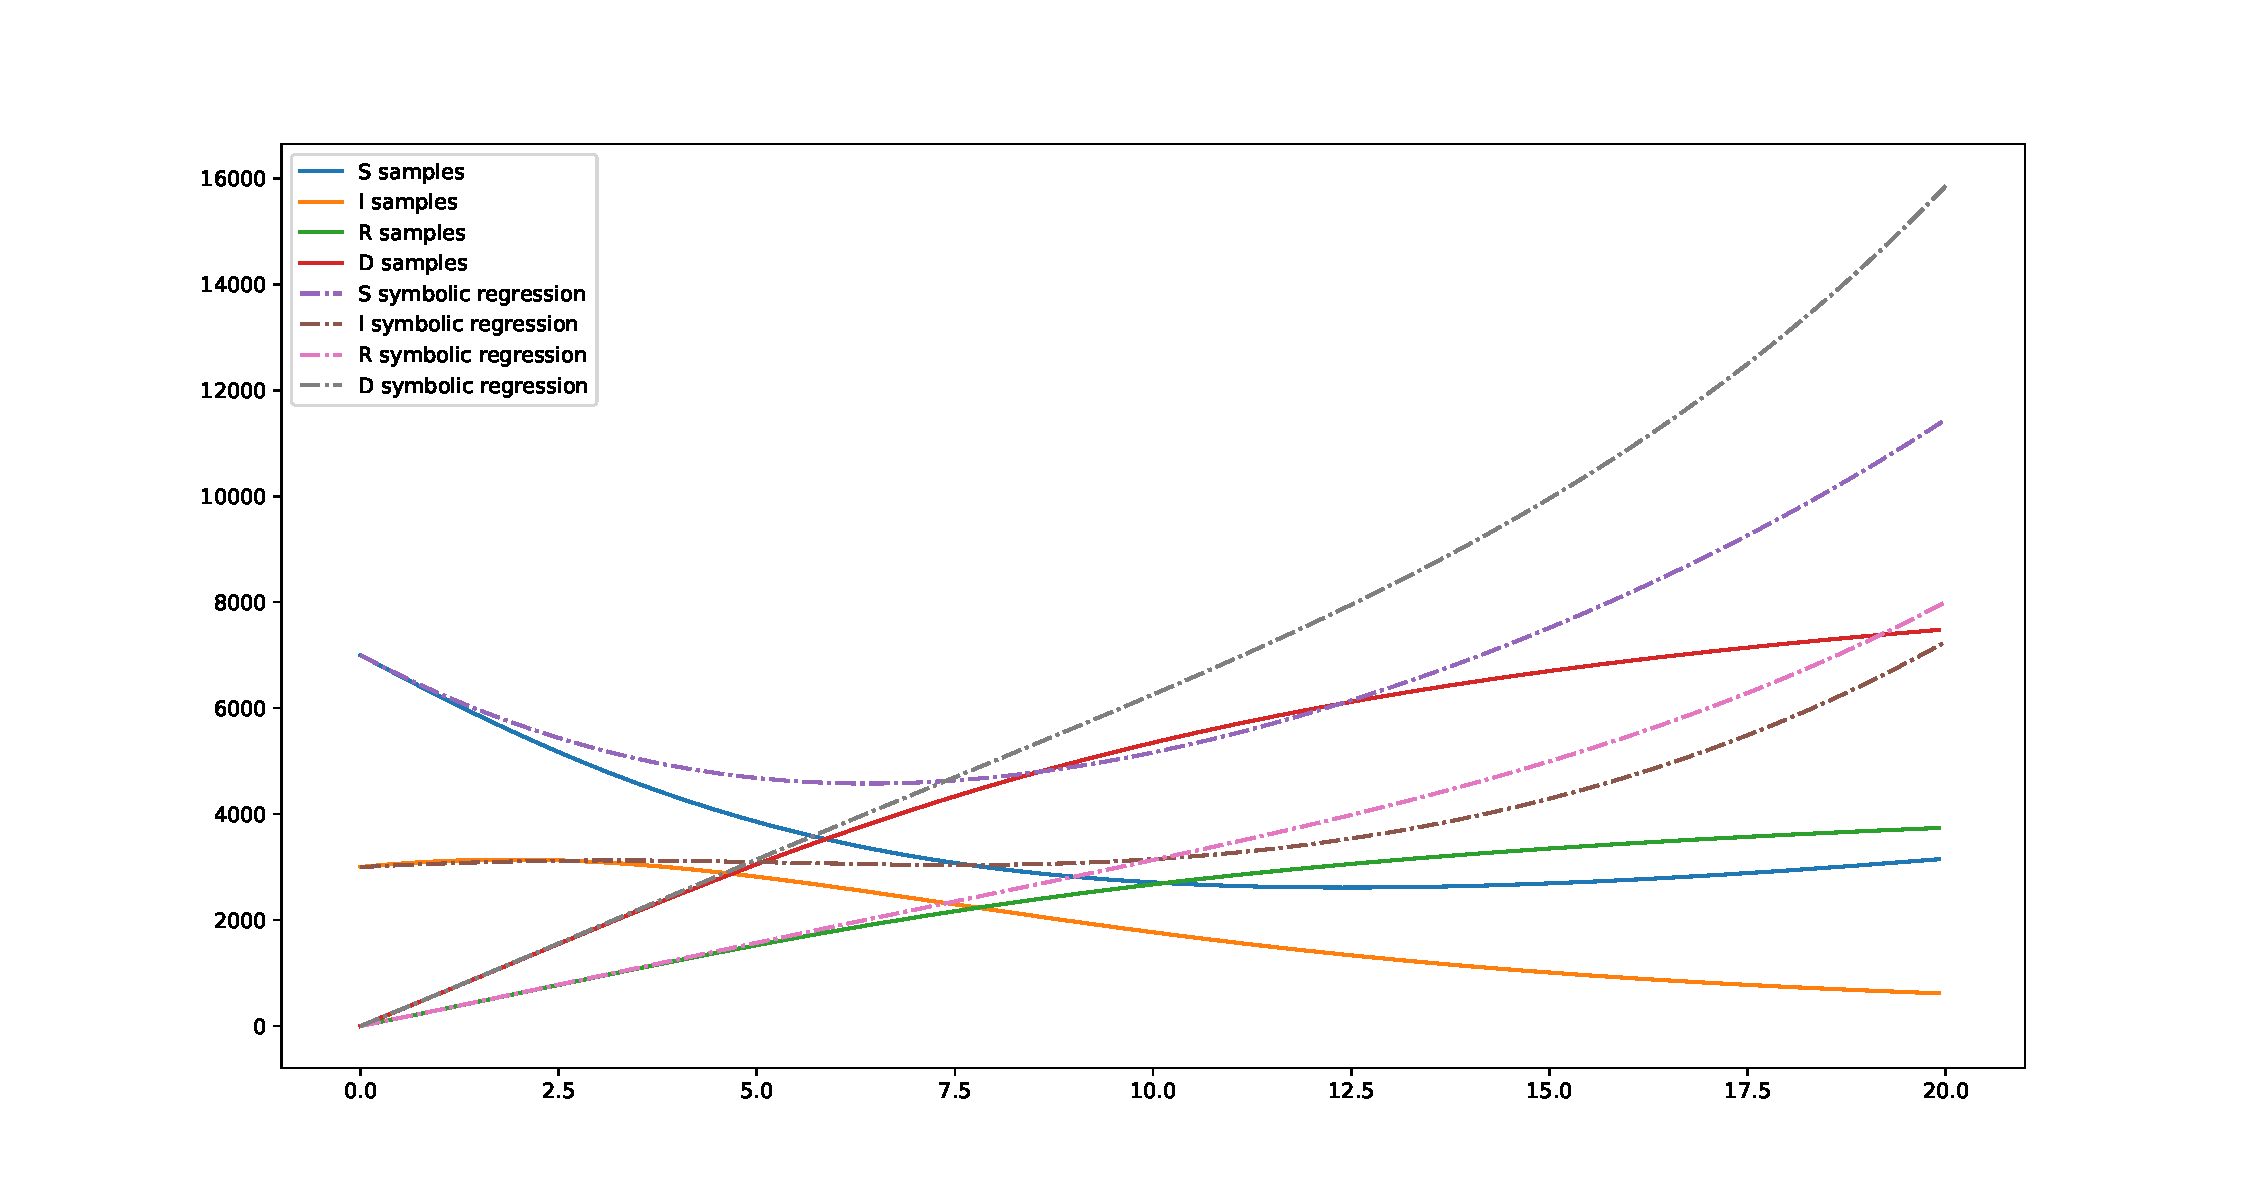
\includegraphics[width=\textwidth]{"figures/final_plot_SIRD_0.05.pdf"}
    \caption{Modelo resultante utilizando datos generados a partir del modelo SIRD con ruido máximo de 5\%.}
    \label{fig:final_plot_SIRD_0.05}
\end{figure}

\begin{figure}[h]
    \centering
    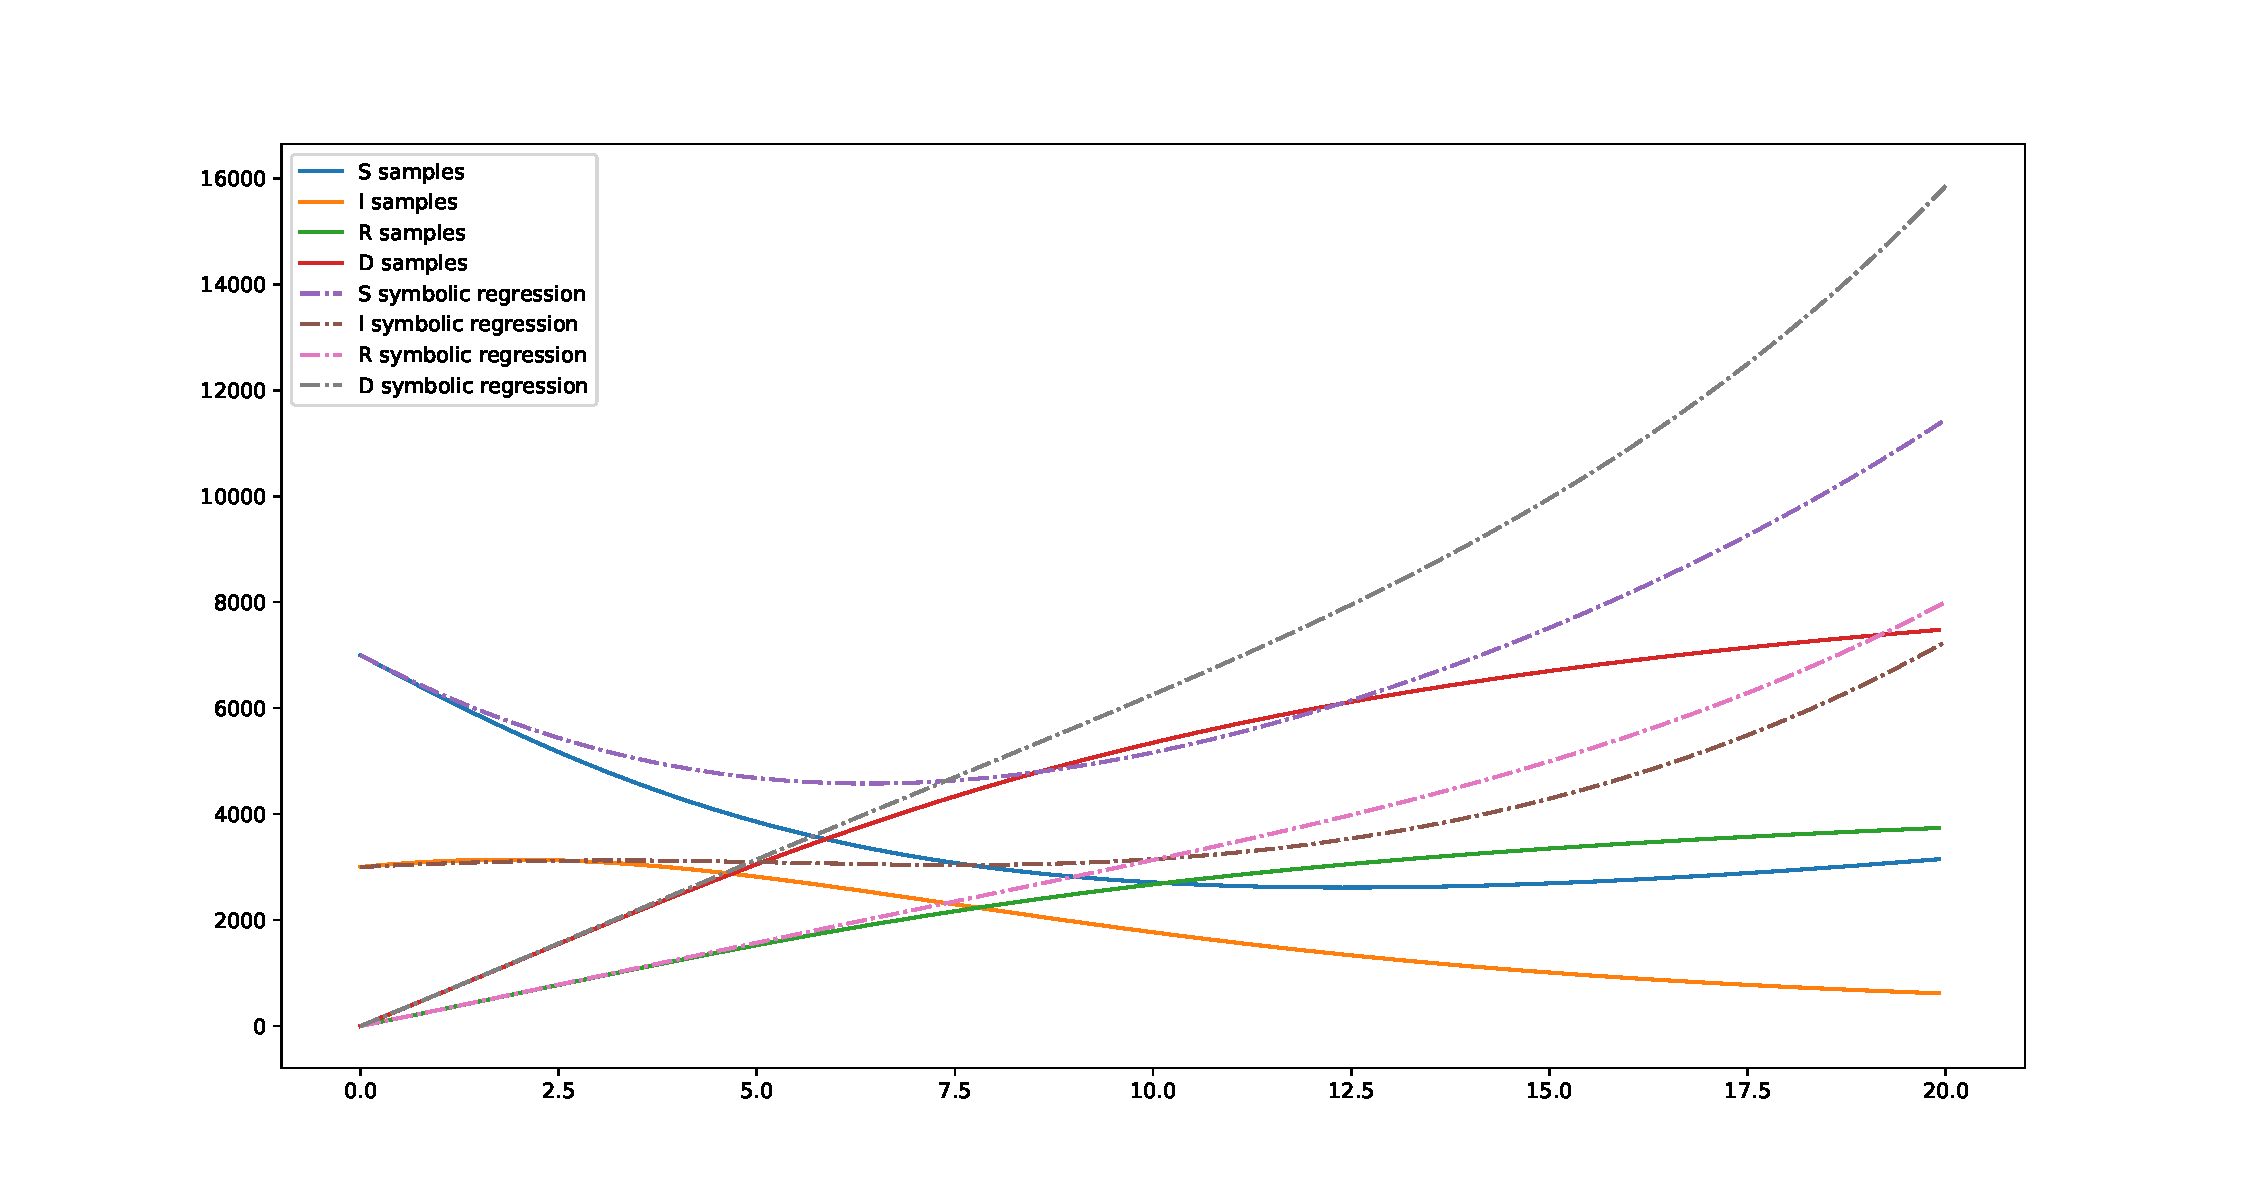
\includegraphics[width=\textwidth]{"figures/final_plot_SIRD_0.1.pdf"}
    \caption{Modelo resultante utilizando datos generados a partir del modelo SIRD con ruido máximo de 10\%.}
    \label{fig:final_plot_SIRD_0.1}
\end{figure}

Si en lugar de utilizar como aproximación el método de diferencias finitas cuando los datos no poseen ruido, se utiliza el sistema original de SIR, se obtiene que la media del valor de la función de ajuste a lo largo de las 30 ejecuciones del experimento es $29.94535$. El valor máximo de la función de ajuste alcanzado fue de $128.83451$ y el mínimo de $2.25834e-14$, en este último la regresión simbólica obtuvo exactamente el sistema utilizado para generar los datos.

A continuación se muestra el experimento realizado a partir de la generación de datos utilizando el sistema SIQRD.

\subsection{SIQRD}

El modelo SIQRD añade al modelo SIRD la posibilidad de aislamiento de una persona, denotado por $Q$, esto modela la situación en que una persona se aisle para no contagiarse o no contagiar a otros \cite{molter2021mathematical}. El sistema se define como:

\begin{align*}
    S' & = -\beta (\frac{S I}{S + I + Q + R + D}) - \alpha S + \delta Q \\
    I' & = \beta (\frac{S I}{S + I + Q + R + D}) - \gamma I - \mu I     \\
    Q' & = \alpha S - \delta Q                                          \\
    R' & = \gamma I                                                     \\
    D' & = \mu I,
\end{align*}

donde $\alpha$ indica la relación con que una persona susceptible es enviada a aislamiento, $\beta$ es el índice de transmisión, $\delta$ indica la relación con que una persona en aislamiento social regresa al grupo de susceptibles, $\gamma$ indica el índice de recuperación y $\mu$ el índice de muerte a causa de la enfermedad.

Se utilizaron como valores de los parámetros $\alpha = 0.2$, $\beta = 0.9$, $\delta = 0.1$, $\gamma = 0.1$ y $\mu = 0.05$ con punto inicial $(5000, 3000, 1000, 0, 0)$ y se integró en el intervalo $0 \leq t \leq 20$ para obtener los datos que aparecen en la imagen \ref{fig:SIQRD} de la página \pageref{fig:SIQRD}. Del conjunto de puntos se seleccionaron 300 muestras como datos para el método de regresión simbólica.

\begin{figure}[h]
    \centering
    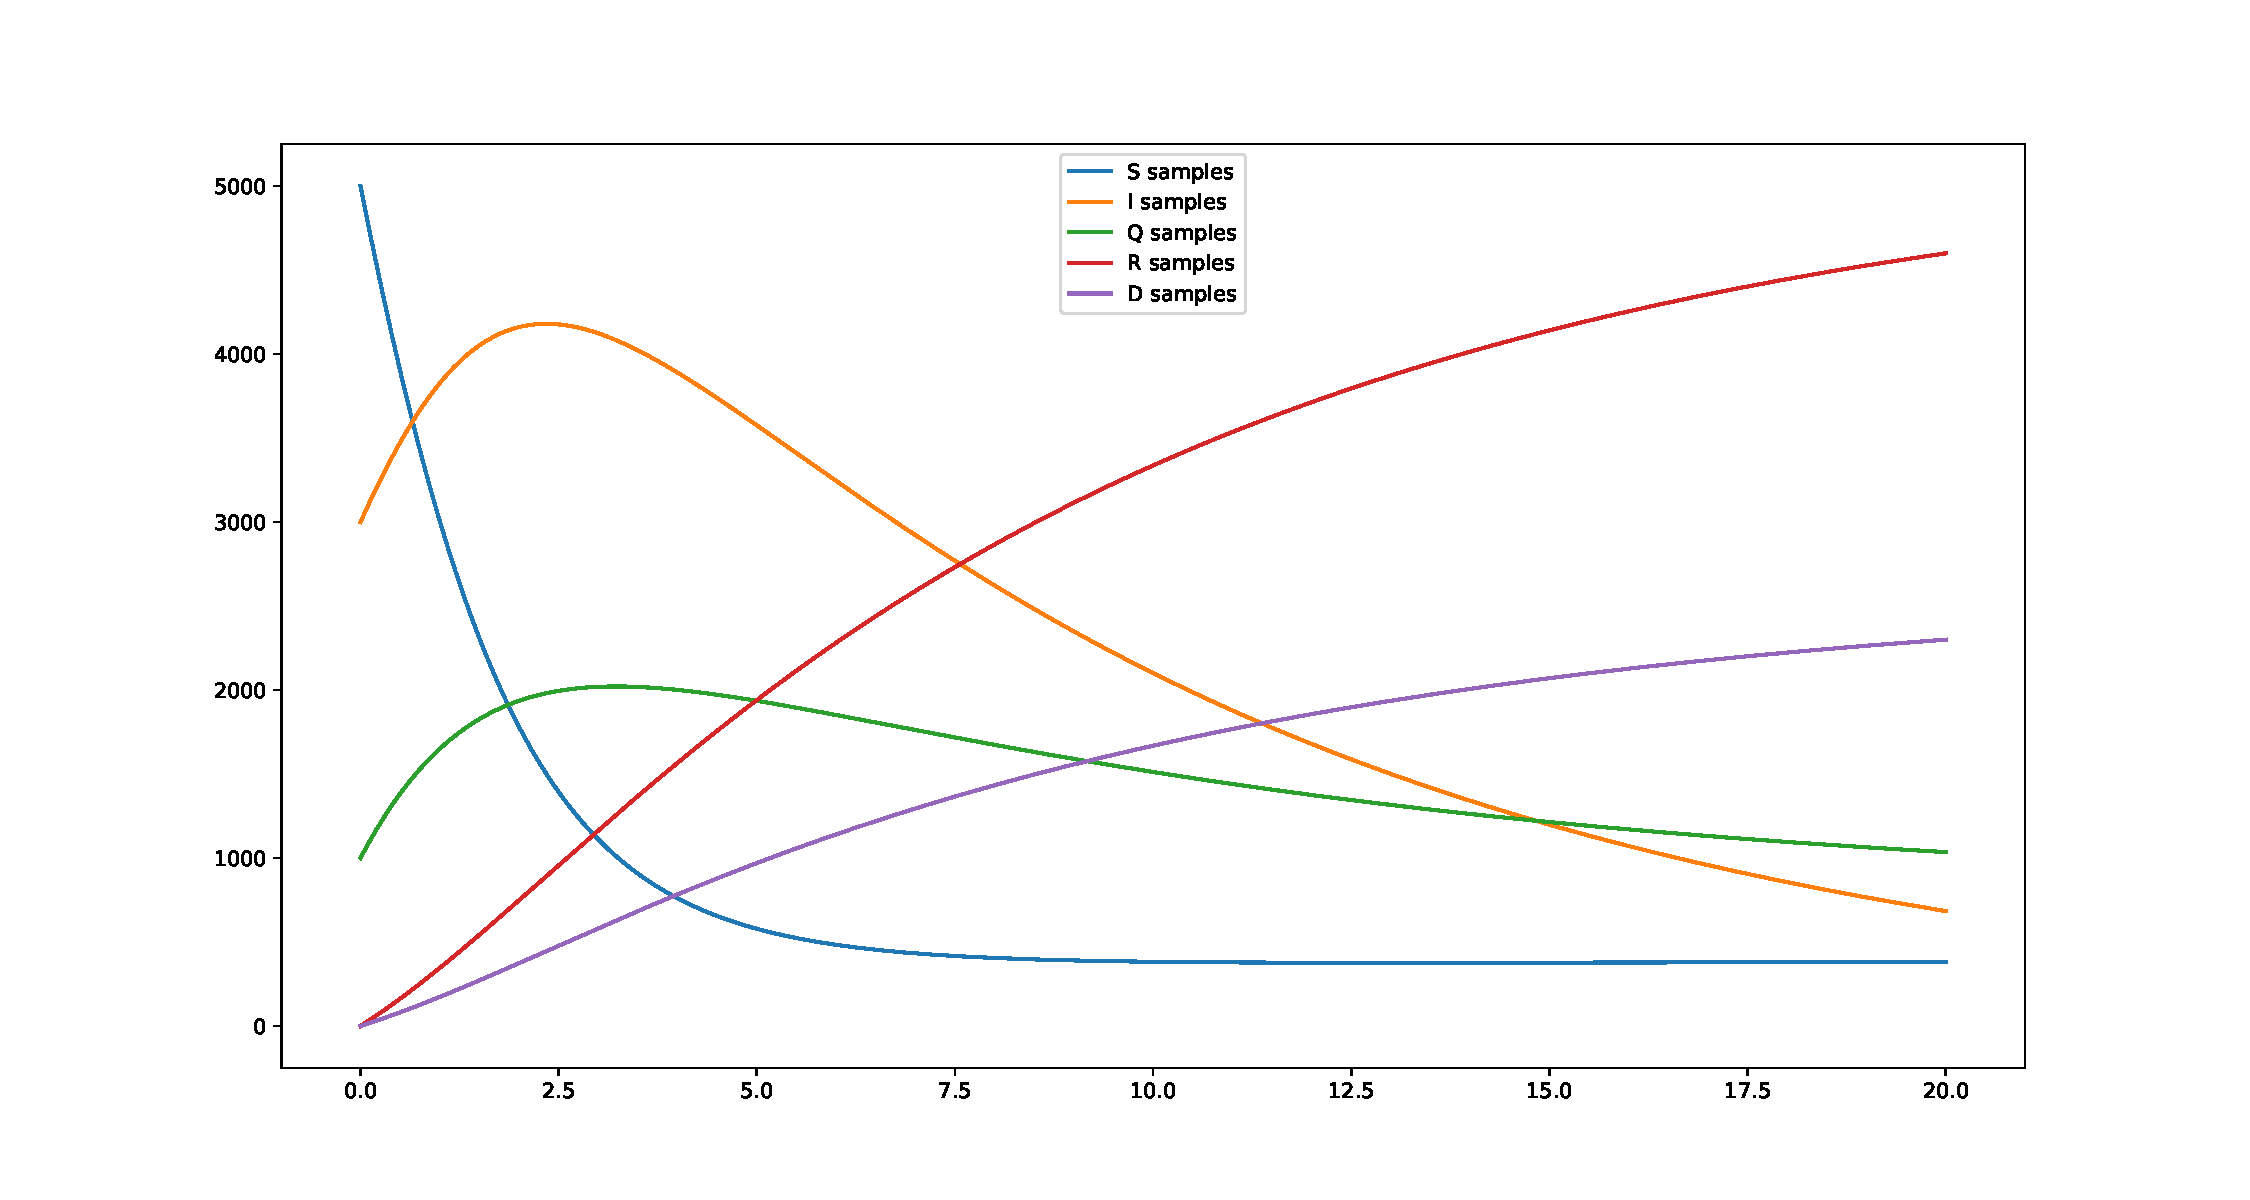
\includegraphics[width=\textwidth]{"figures/SIQRD.pdf"}
    \caption{modelo SIQRD con $\alpha = 0.2$, $\beta = 0.9$, $\delta = 0.1$, $\gamma = 0.1$ y $\mu = 0.05$.}
    \label{fig:SIQRD}
\end{figure}

Los resultados que se obtienen durante las 30 ejecuciones del experimento, utilizando solamente en cada ecuación las variables permitidas según el modelo y además se agrega como varible $N=S + I + Q + R + D$, aparecen en la tabla \ref{table:experiment_SIQRD} de la página \pageref{table:experiment_SIQRD}. Si se permite cualquier variable del modelo en cualquier ecuación del sistema se obtienen los datos que aparecen en la tabla \ref{table:experiment_SIQRD_all} de la página \pageref{table:experiment_SIQRD_all}.

\begin{table}[!h]
    \centering
    \caption{Resultados que se obtienen en el modelo SIQRD restringiendo las variables que aparecen en cada ecuación.}
    \begin{tabular}{|c|c|c|c|}
        \hline
               & \textbf{ruido de 0\%} & \textbf{ruido de 5\%} & \textbf{ruido de 10\%} \\
        \hline
        media  & 7.47098               & 35.17738              & 38.70691               \\
        \hline
        mínimo & 1.35941               & 7.96579               & 12.25428               \\
        \hline
        máximo & 49.24056              & 99.18317              & 197.34403              \\
        \hline
    \end{tabular}

    \begin{tabular}{|c|c|c|c|c|c|}
        \hline
                             & \textbf{ruido de 0\%} & \textbf{ruido de 5\%} & \textbf{ruido de 10\%} \\
        \hline
        cantidad de sistemas & 29                    & 22                    & 22                     \\
        \hline
        original             & 76.49518              & 517.5006              & 338.54534              \\
        \hline
        original con ruido   & 76.49518              & 536.1417              & 395.29378              \\
        \hline
        spline               & 76.49518              & 515.51251             & 338.39969              \\
        \hline
        otro método          & 698.3556              & 919.78558             & 747.2666               \\
        \hline
    \end{tabular}
    \label{table:experiment_SIQRD}
\end{table}

\begin{table}[!h]
    \centering
    \caption{Resultados que se obtienen en el modelo SIQRD sin restringir las variables que aparecen en cada ecuación.}
    \begin{tabular}{|c|c|c|c|}
        \hline
               & \textbf{ruido de 0\%} & \textbf{ruido de 5\%} & \textbf{ruido de 10\%} \\
        \hline
        media  & 5.00116               & 34.76361              & 33.05852               \\
        \hline
        mínimo & 2.43638               & 8.78968               & 13.28306               \\
        \hline
        máximo & 7.84816               & 80.32846              & 83.9451                \\
        \hline
    \end{tabular}

    \begin{tabular}{|c|c|c|c|c|c|}
        \hline
                             & \textbf{ruido de 0\%} & \textbf{ruido de 5\%} & \textbf{ruido de 10\%} \\
        \hline
        cantidad de sistemas & 29                    & 20                    & 19                     \\
        \hline
        original             & 69.88262              & 357.61219             & 259.33185              \\
        \hline
        original con ruido   & 69.88262              & 372.24346             & 312.84906              \\
        \hline
        spline               & 69.88262              & 356.83797             & 253.63394              \\
        \hline
        otro método          & 730.13032             & 901.498               & 735.24475              \\
        \hline
    \end{tabular}
    \label{table:experiment_SIQRD_all}
\end{table}

Con este experimento se obtiene que los sistemas generados por la regresión simbólica ajustan los datos mientras estos no posean ruido. Los datos que se obtienen de la integración del sistema resultante de la regresión simbólica se asemejan a los datos de la integración del sistema seleccionado para la realización del experimento pero la aparición de ruido afecta el ajuste de los datos. Los datos que se obtienen de la integración del sistema obtenido a partir de un conjunto de datos con ruido máximo de 5\% obtiene peores resultados que si se utiliza como ruido máximo 10\%. Esto se puede deber a un mal ajuste del parámetro de suavizado utilizado en spline de suavizado.

En las figuras \ref{fig:final_plot_SIQRD_0.0} de la página \pageref{fig:final_plot_SIQRD_0.0}, \ref{fig:final_plot_SIQRD_0.05} de la página \pageref{fig:final_plot_SIQRD_0.05} y \ref{fig:final_plot_SIQRD_0.1} de la página \pageref{fig:final_plot_SIQRD_0.1} se pueden ver los datos originales comparados con los datos obtenidos del mejor resultado generado por la regresión simbólica restringiendo las variables que pueden existir en cada ecuación.

\begin{figure}[h]
    \centering
    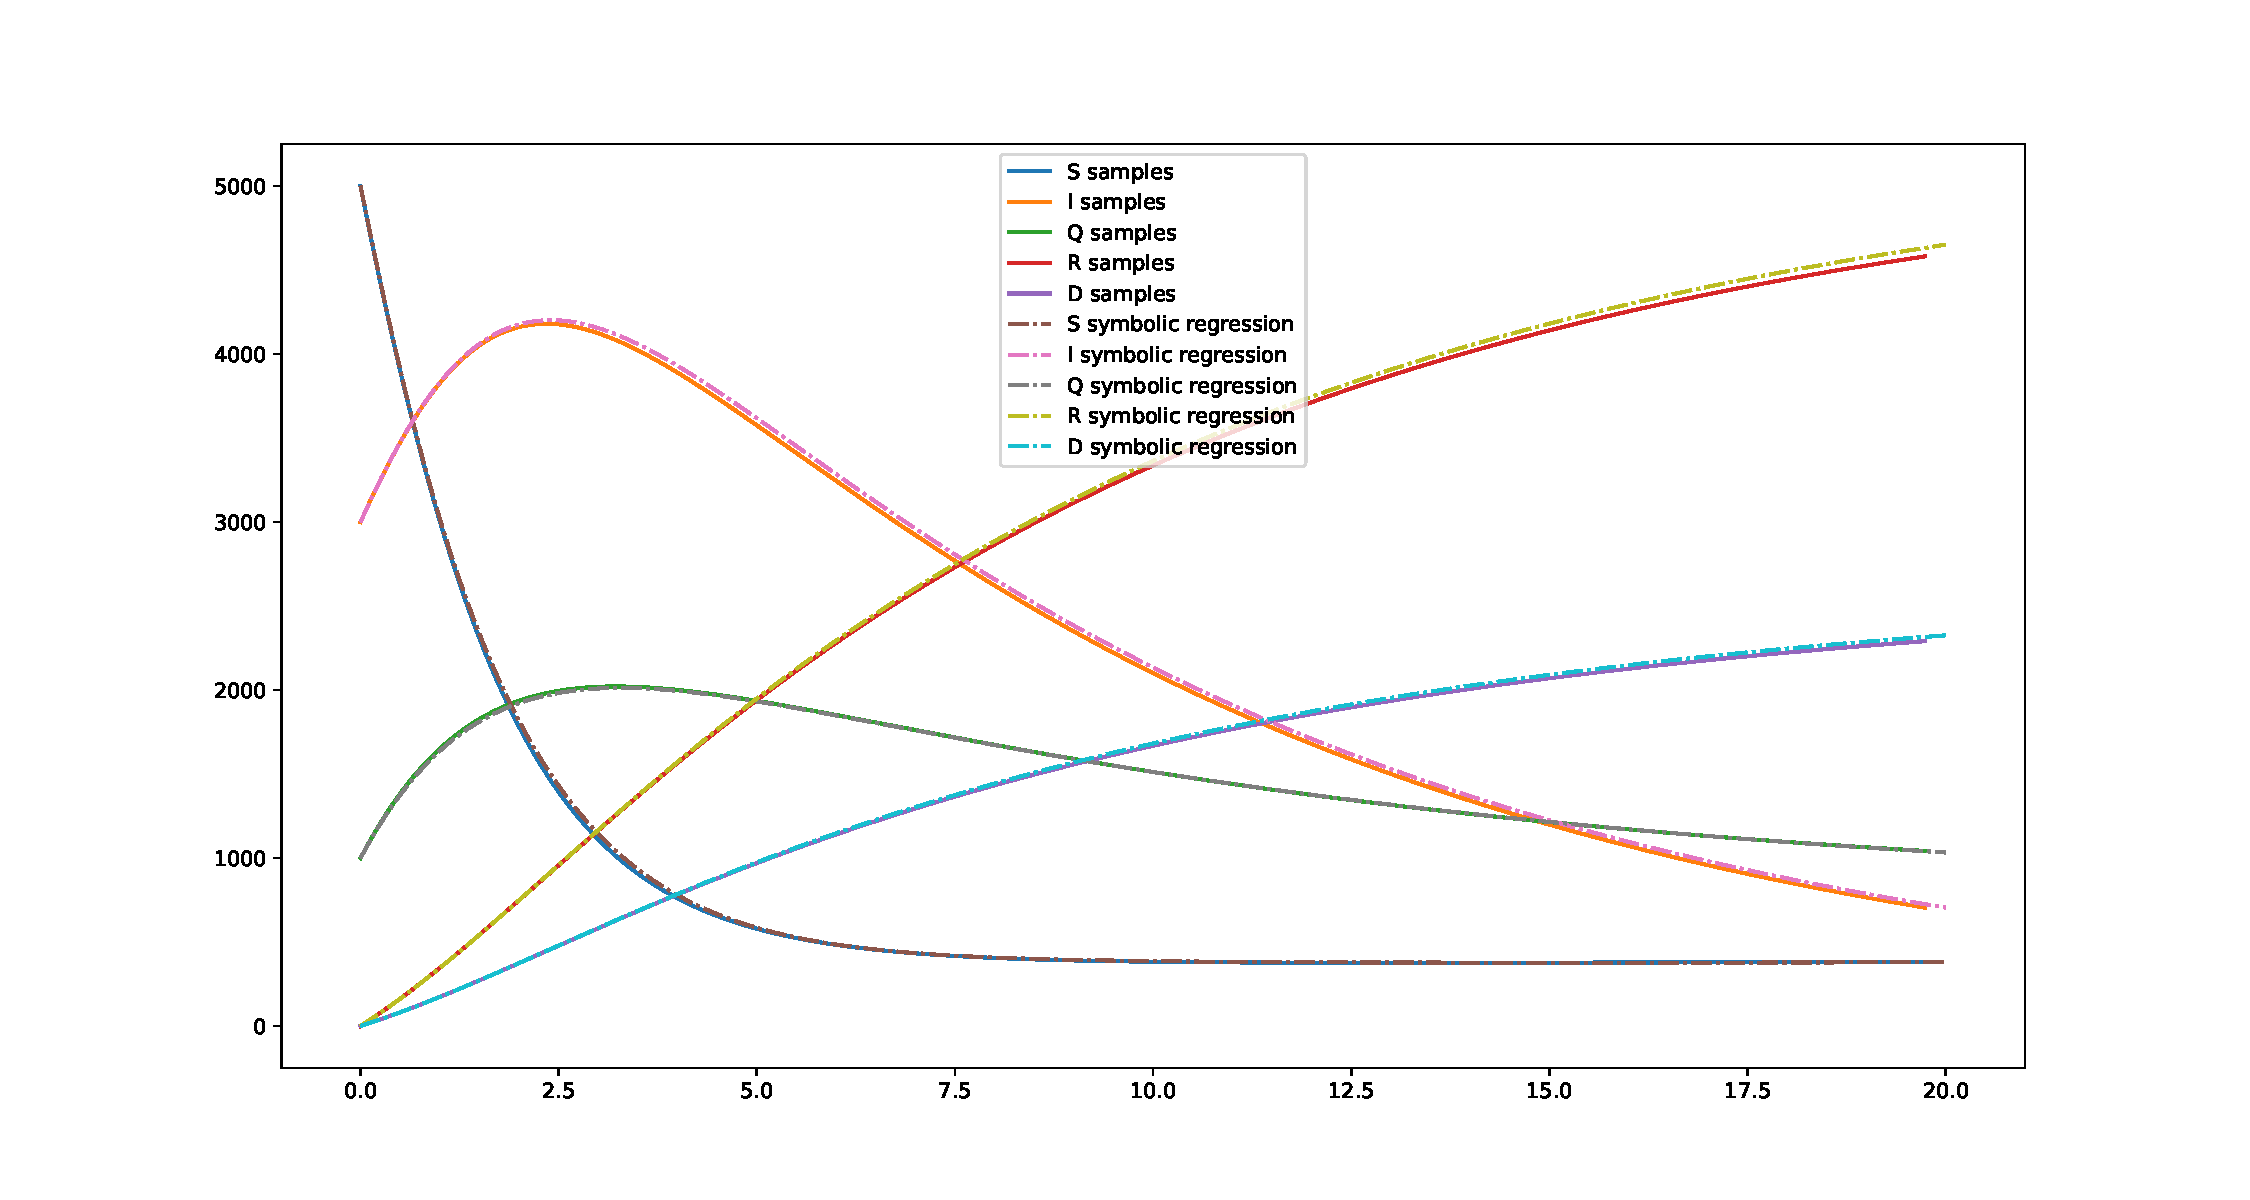
\includegraphics[width=\textwidth]{"figures/final_plot_SIQRD_0.0.pdf"}
    \caption{Modelo resultante utilizando datos generados a partir del modelo SIQRD con ruido máximo de 0\%.}
    \label{fig:final_plot_SIQRD_0.0}
\end{figure}

\begin{figure}[h]
    \centering
    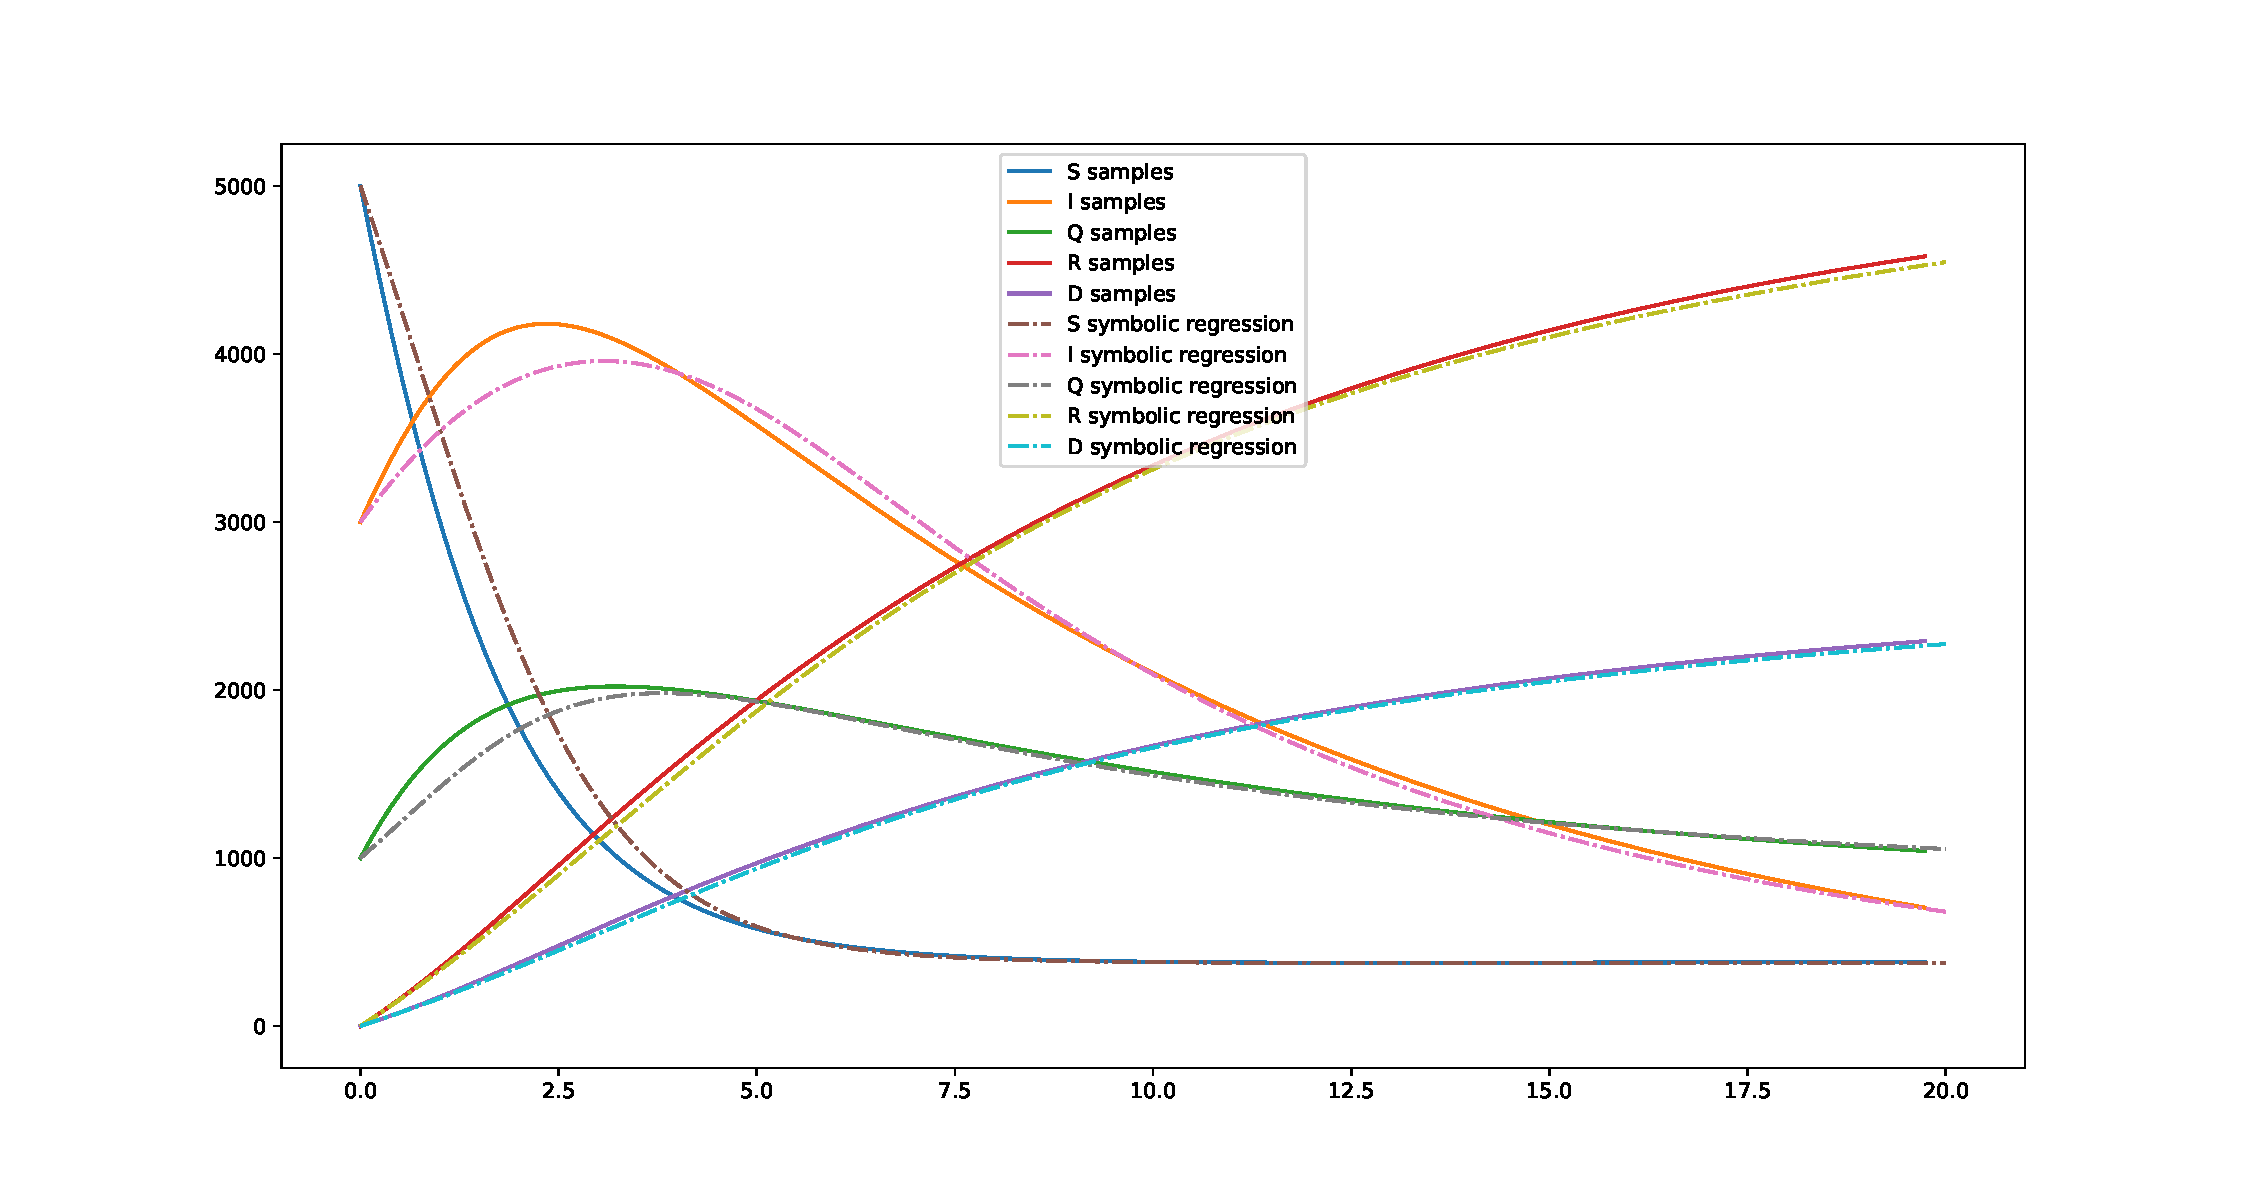
\includegraphics[width=\textwidth]{"figures/final_plot_SIQRD_0.05.pdf"}
    \caption{Modelo resultante utilizando datos generados a partir del modelo SIQRD con ruido máximo de 5\%.}
    \label{fig:final_plot_SIQRD_0.05}
\end{figure}

\begin{figure}[h]
    \centering
    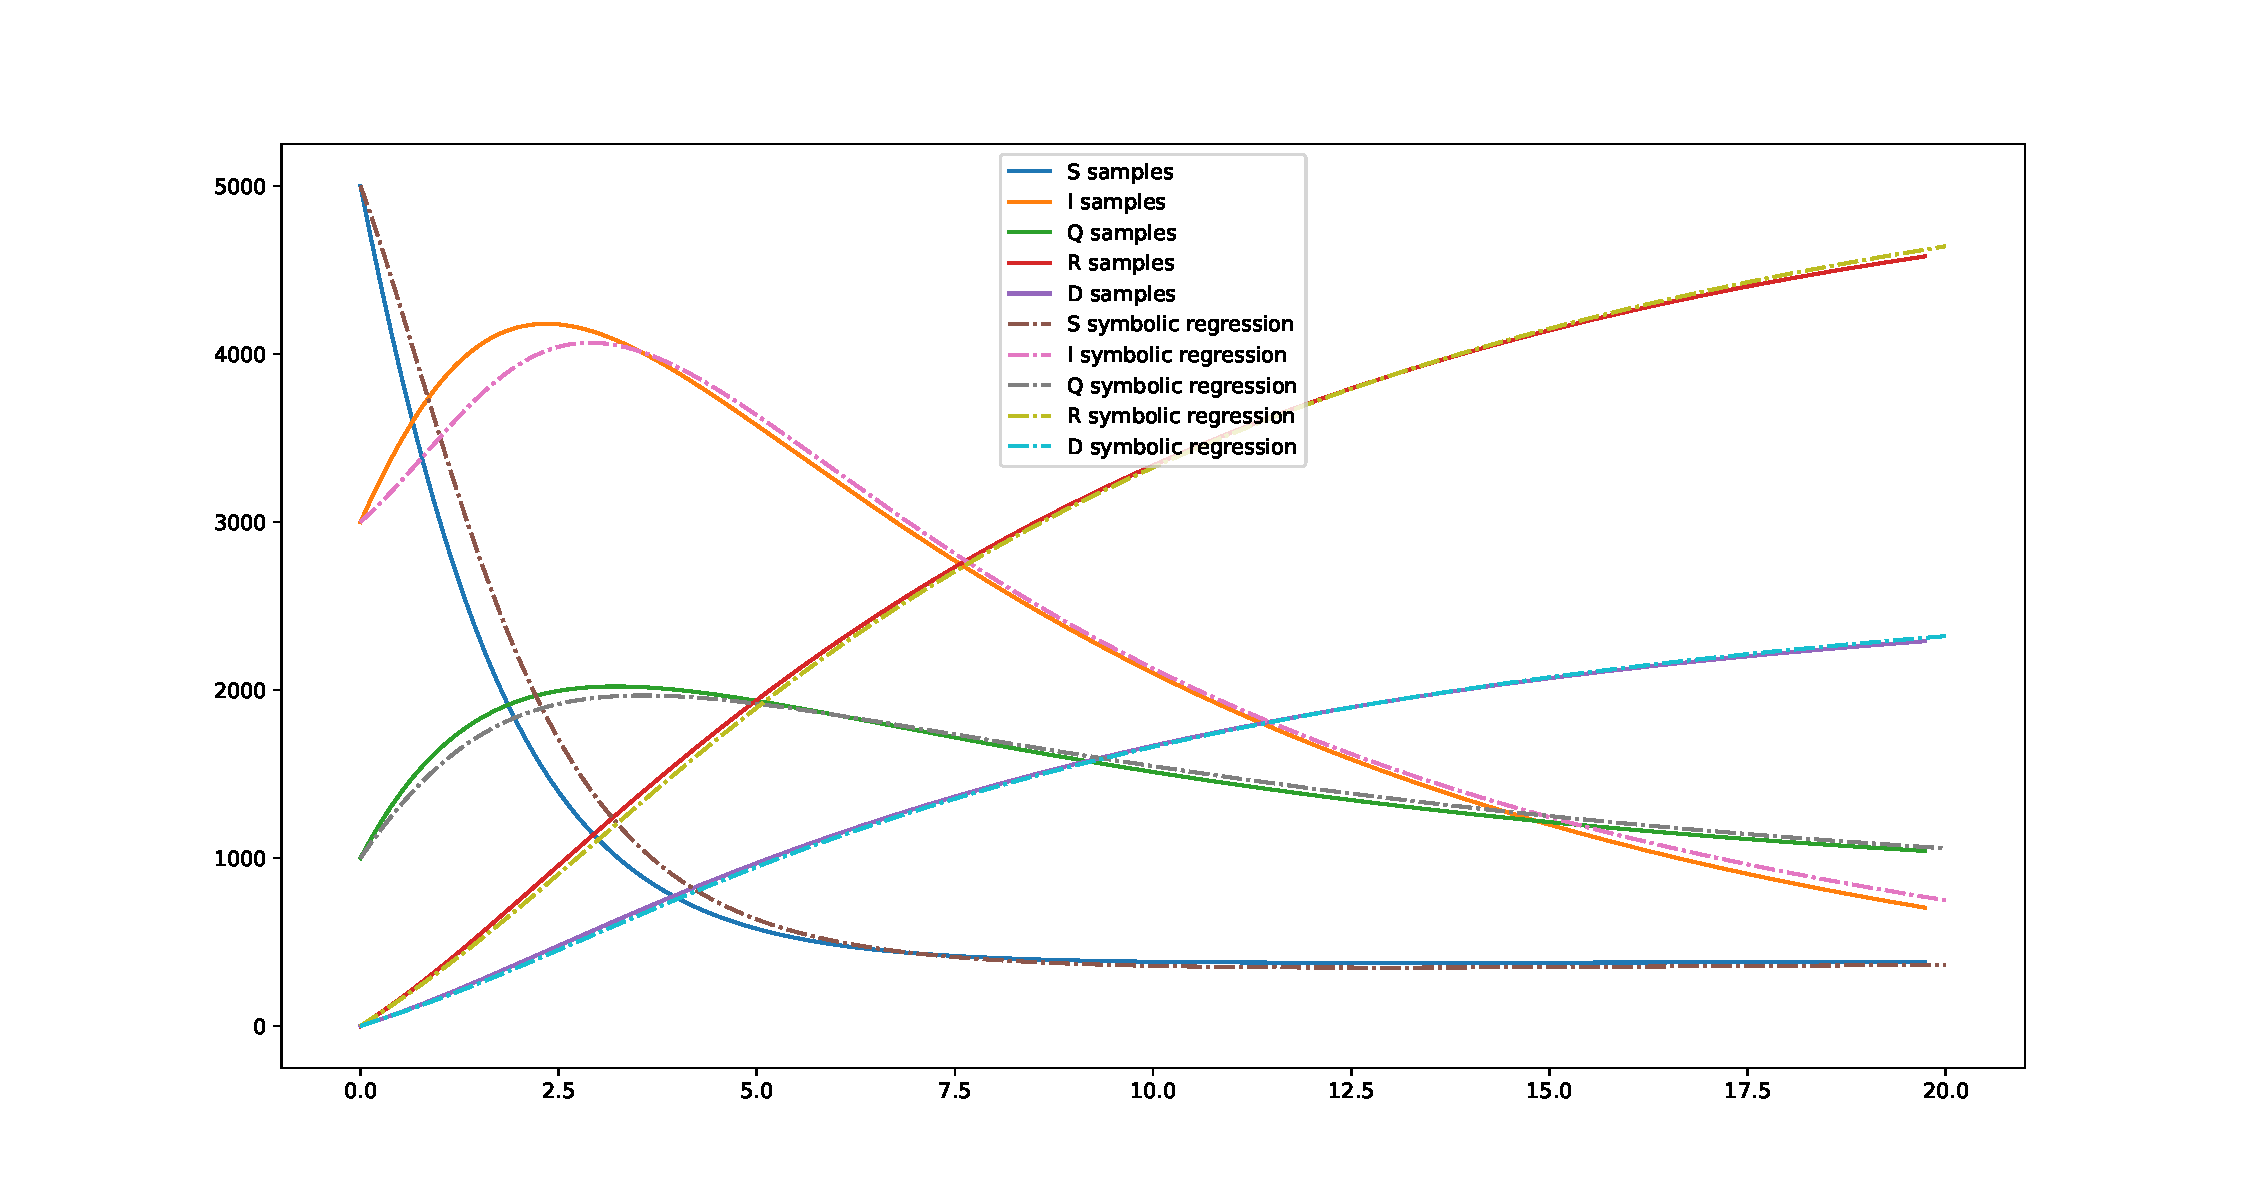
\includegraphics[width=\textwidth]{"figures/final_plot_SIQRD_0.1.pdf"}
    \caption{Modelo resultante utilizando datos generados a partir del modelo SIQRD con ruido máximo de 10\%.}
    \label{fig:final_plot_SIQRD_0.1}
\end{figure}

Si en lugar de utilizar como aproximación el método de diferencias finitas cuando los datos no poseen ruido, se utiliza el sistema original de SIR, se obtiene que la media del valor de la función de ajuste a lo largo de las 30 ejecuciones del experimento es $6.01436$. El valor máximo de la función de ajuste alcanzado fue de $48.48072$ y el mínimo de $1.42392e-14$, en este último la regresión simbólica obtuvo el sistema:

\begin{align*}
    S' & = -0.1 * S -0.1 * S + -0.0001 * (I * S) + 0.1 * Q \\
    I' & = -0.075 * I + 0.0001 * (S * I) -0.075 * I        \\
    Q' & = -0.1 * Q + 0.2 * S                              \\
    R' & = -0.1 * -I                                       \\
    D' & = 0.025 * I + 0.025 * I,
\end{align*}

que es igual al sistema original si se asume $\frac{\beta}{N} = 0.0001$.

A continuación se muestra el experimento realizado a partir de la generación de datos utilizando el sistema SVVEIR.

\subsection{SVVEIR}

El modelo SVVEIR describe un escenario de una posible enfermedad en la sociedad de Bangladesh. En el modelo se plantea un conjunto $S$ de individuos que no se han infectado aún, $V_1$ y $V_2$ son los individuos que han recibido la primera y segunda vacuna, respectivamente. Las personas infectadas pero que aún no han desarrollado síntomas se definen como expuestos y se encuentran representados por el conjunto $E$. Los parámetros $I$ y $R$ identifican los mismos conjuntos que en el modelo SIR \cite{kuddus2021mathematical}. El sistema se define como:


\begin{align*}
    N    & = S + V_1 + V_2 + E + I + R                                        \\
    S'   & = \mu * N - \beta * \frac{I}{N} * S - n * S - \mu * S + \rho * V_1 \\
    V_1' & = n * S - \rho * V_1 - \sigma * V_1 - \mu * V_1                    \\
    V_2' & = \sigma * V_1 - \omega * V_2 - \mu * V_2                          \\
    E'   & = \beta * I / N * S - \alpha * E - \mu * E                         \\
    I'   & = \alpha * E - \gamma * I - \delta * I - \mu * I                   \\
    R'   & = \gamma * I + \omega * V_2 - \mu * R,
\end{align*}

donde $\alpha$ indica la relación de personas expuestas que pasan a estar infectados, $\beta$ es el índice de transmisión de la enfermedad, $\delta$ es el índice de muerte debido a la enfermedad mientras que $\mu$ es el índice de muerte por causas naturales. El índice de recuperación de la enfermedad se representa mediante el parámetro $\gamma$. El parámetro $n$ muestra el índice de personas susceptibles que reciben la primera dosis de la vacuna y $\rho$ describe la relación de personas con una sola dosis de la vacuna que regresan al grupo de susceptibles. La cantidad de personas que reciben la segunda dosis se refleja en el parámetro $\sigma$ y $\omega$ es el parámetro que muestra la relación de personas con dos dosis de la vacuna que pasan a recuperados.

Se utilizaron como valores de los parámetros $\alpha = 0.1$, $\beta = 0.7$, $\delta = 0.0005$, $\gamma = 0.05$, $\mu = 0.01$, $n = 0.2$, $\rho = 0.01$, $\omega = 0.05$ y $\sigma = 0.2$ con punto inicial $(5000, 1000, 0, 2000, 1000, 500)$ y se integró en el intervalo $0 \leq t \leq 20$ para obtener los datos que aparecen en la figura \ref{fig:SVVEIR} de la página \pageref{fig:SVVEIR}. Del conjunto de puntos se seleccionaron 300 muestras como datos para el método de regresión simbólica.

\begin{figure}[h]
    \centering
    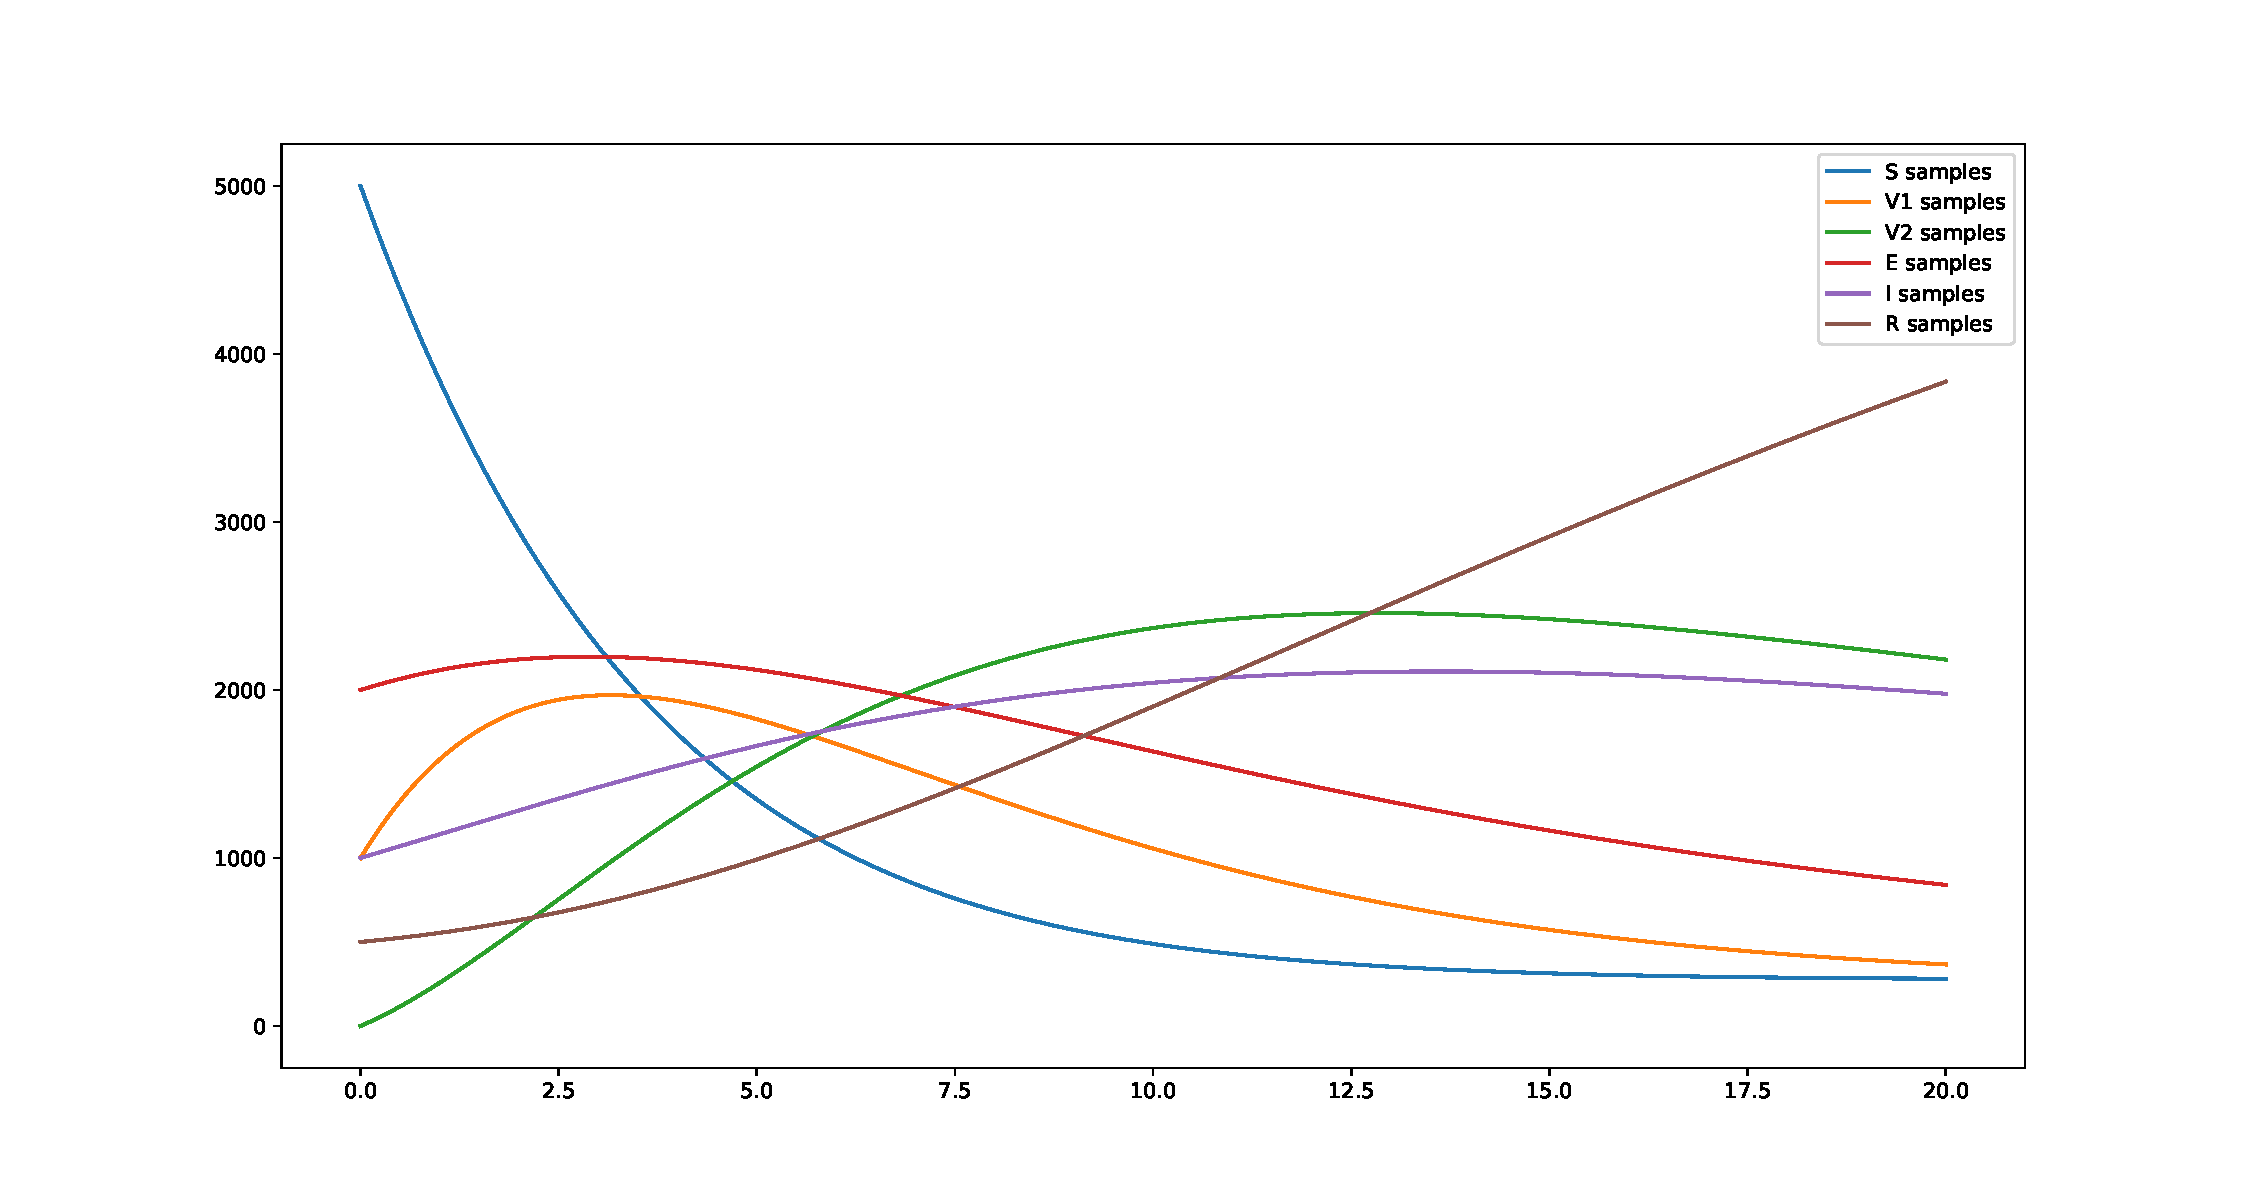
\includegraphics[width=\textwidth]{"figures/SVVEIR.pdf"}
    \caption{modelo SVVEIR con $\alpha = 0.1$, $\beta = 0.7$, $\delta = 0.0005$, $\gamma = 0.05$, $\mu = 0.01$, $n = 0.2$, $\rho = 0.01$, $\omega = 0.05$ y $\sigma = 0.2$.}
    \label{fig:SVVEIR}
\end{figure}

Los resultados que se obtienen durante las 30 ejecuciones del experimento, utilizando solamente en cada ecuación las variables permitidas según el modelo y además se agrega como varible $N=S + V_1 + V_2 + E + I + R$, aparecen en la tabla \ref{table:experiment_SVVEIR} de la página \pageref{table:experiment_SVVEIR}. Si se permite cualquier variable del modelo en cualquier ecuación del sistema se obtienen los datos que aparecen en la tabla \ref{table:experiment_SVVEIR_all} de la página \pageref{table:experiment_SVVEIR_all}.

\begin{table}[!h]
    \centering
    \caption{Resultados que se obtienen en el modelo SVVEIR restringiendo las variables que aparecen en cada ecuación.}
    \begin{tabular}{|c|c|c|c|}
        \hline
               & \textbf{ruido de 0\%} & \textbf{ruido de 5\%} & \textbf{ruido de 10\%} \\
        \hline
        media  & 3.64426               & 13.57802              & 16.12164               \\
        \hline
        mínimo & 1.30096               & 9.50931               & 12.69225               \\
        \hline
        máximo & 14.28797              & 29.02875              & 25.4523                \\
        \hline
    \end{tabular}

    \begin{tabular}{|c|c|c|c|c|c|}
        \hline
                             & \textbf{ruido de 0\%} & \textbf{ruido de 5\%} & \textbf{ruido de 10\%} \\
        \hline
        cantidad de sistemas & 30                    & 30                    & 29                     \\
        \hline
        original             & 26.41261              & 121.61259             & 94.25209               \\
        \hline
        original con ruido   & 26.41261              & 146.93245             & 165.1642               \\
        \hline
        spline               & 26.41261              & 121.72339             & 94.75343               \\
        \hline
        otro método          & 1431.78292            & 1415.93366            & 1612.23507             \\
        \hline
    \end{tabular}
    \label{table:experiment_SVVEIR}
\end{table}

\begin{table}[!h]
    \centering
    \caption{Resultados que se obtienen en el modelo SVVEIR sin restringir las variables que aparecen en cada ecuación.}
    \begin{tabular}{|c|c|c|c|}
        \hline
               & \textbf{ruido de 0\%} & \textbf{ruido de 5\%} & \textbf{ruido de 10\%} \\
        \hline
        media  & 8.30945               & 15.87176              & 17.95833               \\
        \hline
        mínimo & 1.76748               & 10.78393              & 12.29942               \\
        \hline
        máximo & 45.85105              & 47.08811              & 44.09112               \\
        \hline
    \end{tabular}

    \begin{tabular}{|c|c|c|c|c|c|}
        \hline
                             & \textbf{ruido de 0\%} & \textbf{ruido de 5\%} & \textbf{ruido de 10\%} \\
        \hline
        cantidad de sistemas & 30                    & 28                    & 30                     \\
        \hline
        original             & 146.5678              & 215.51733             & 173.10665              \\
        \hline
        original con ruido   & 146.5678              & 234.37447             & 230.006                \\
        \hline
        spline               & 146.5678              & 216.31001             & 172.30783              \\
        \hline
        otro método          & 1433.89796            & 1355.59667            & 1654.19469             \\
        \hline
    \end{tabular}
    \label{table:experiment_SVVEIR_all}
\end{table}

Con este experimento se obtiene que los sistemas generados por la regresión simbólica ajustan los datos mientras estos no posean ruido. Los datos que se obtienen de la integración del sistema resultante de la regresión simbólica se asemejan a los datos de la integración del sistema seleccionado para la realización del experimento pero la aparición de ruido afecta el ajuste de los datos.

En las figuras \ref{fig:final_plot_SVVEIR_0.0} de la página \pageref{fig:final_plot_SVVEIR_0.0}, \ref{fig:final_plot_SVVEIR_0.05} de la página \pageref{fig:final_plot_SVVEIR_0.05} y \ref{fig:final_plot_SVVEIR_0.1} de la página \pageref{fig:final_plot_SVVEIR_0.1} se pueden ver los datos originales comparados con los datos obtenidos del mejor resultado generado por la regresión simbólica restringiendo las variables que pueden existir en cada ecuación.

\begin{figure}[h]
    \centering
    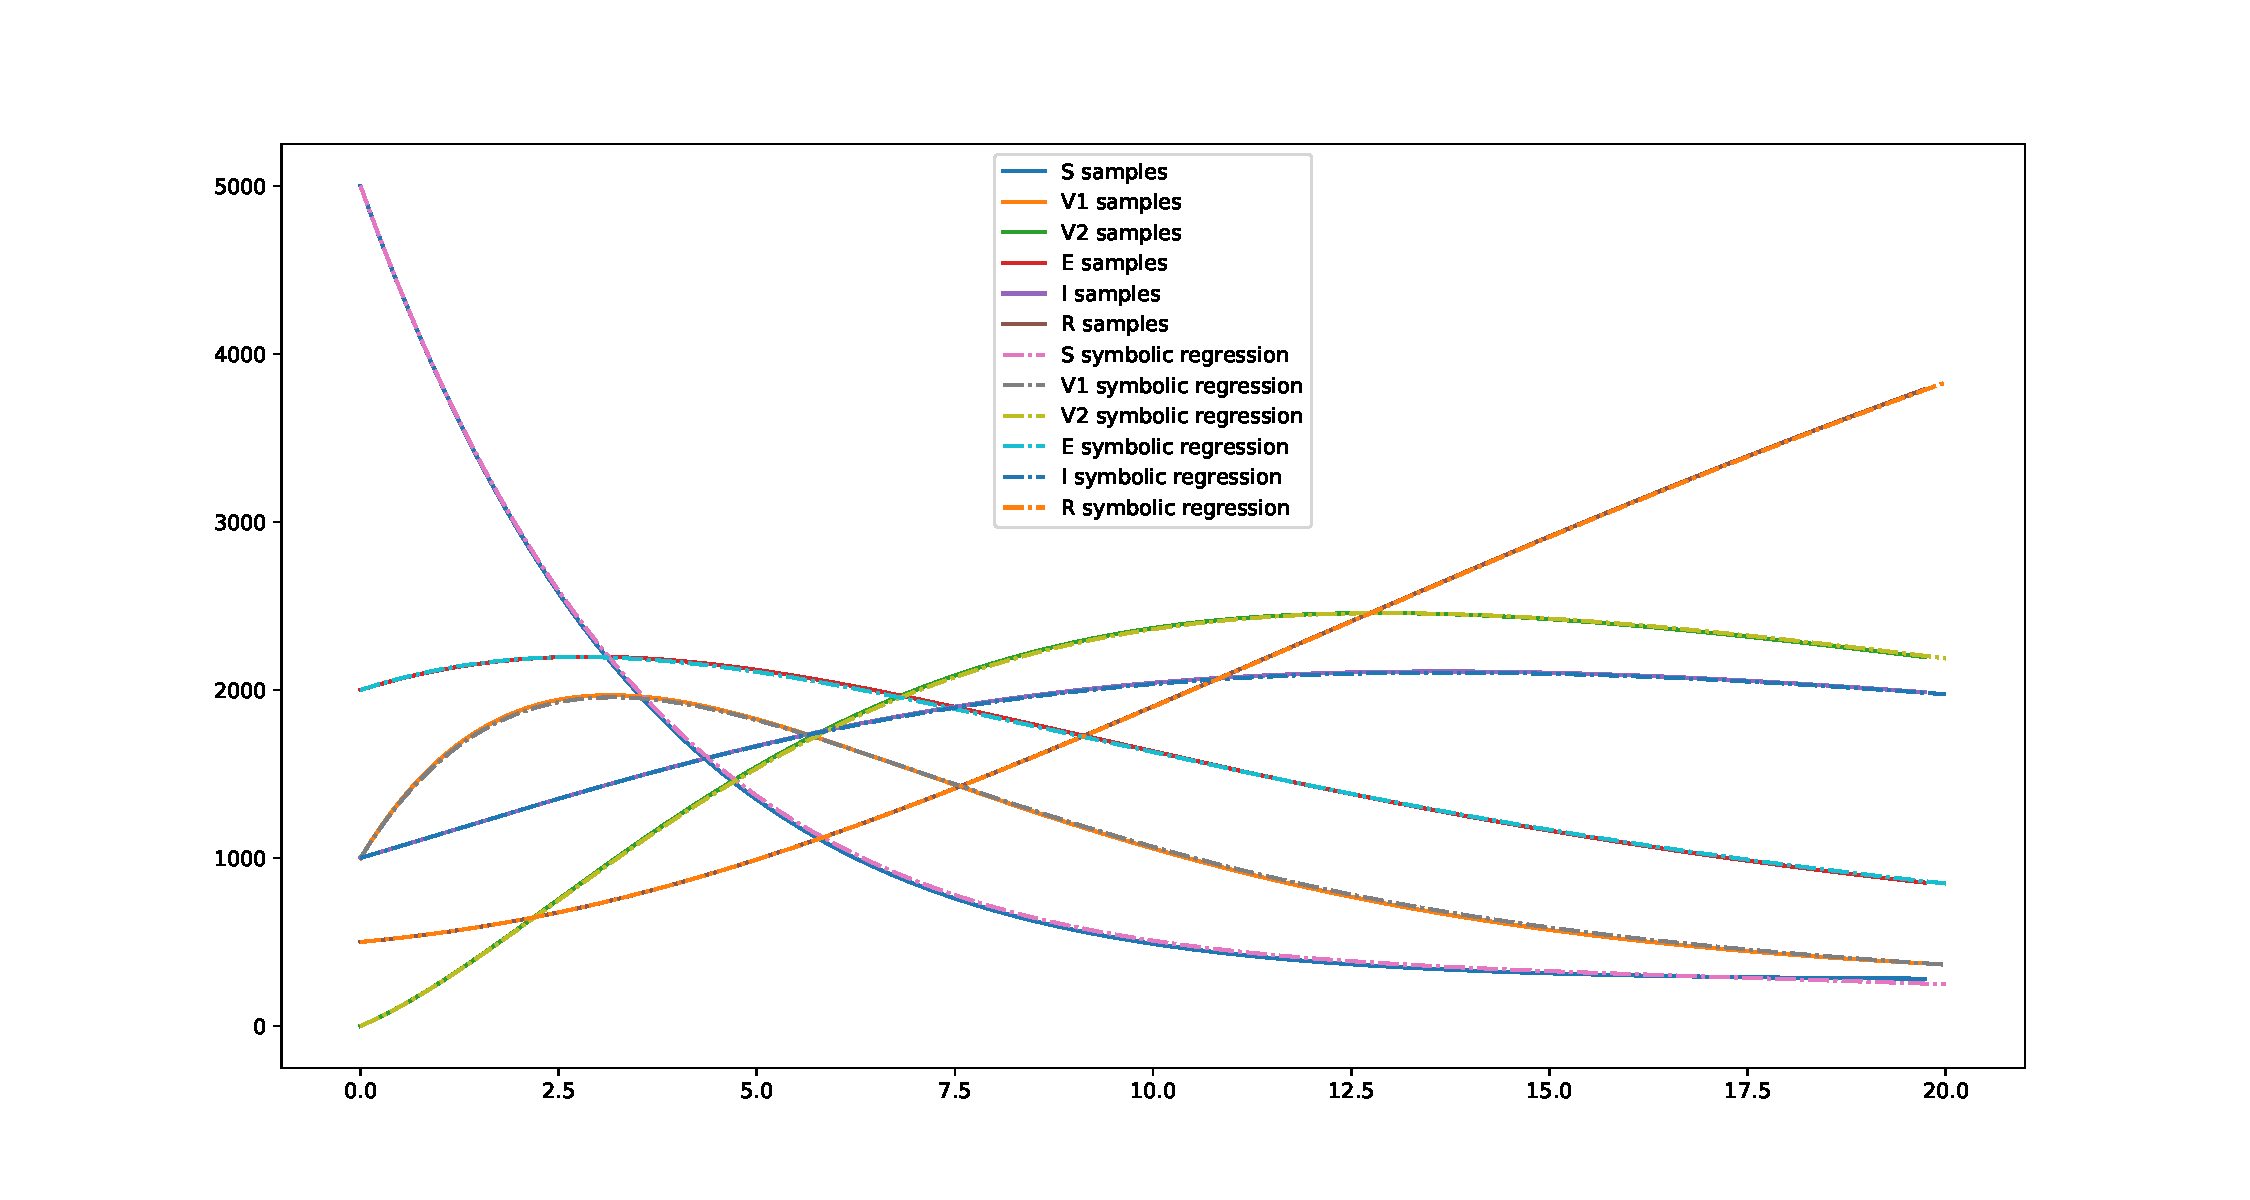
\includegraphics[width=\textwidth]{"figures/final_plot_SVVEIR_0.0.pdf"}
    \caption{Modelo resultante utilizando datos generados a partir del modelo SVVEIR con ruido máximo de 0\%.}
    \label{fig:final_plot_SVVEIR_0.0}
\end{figure}

\begin{figure}[h]
    \centering
    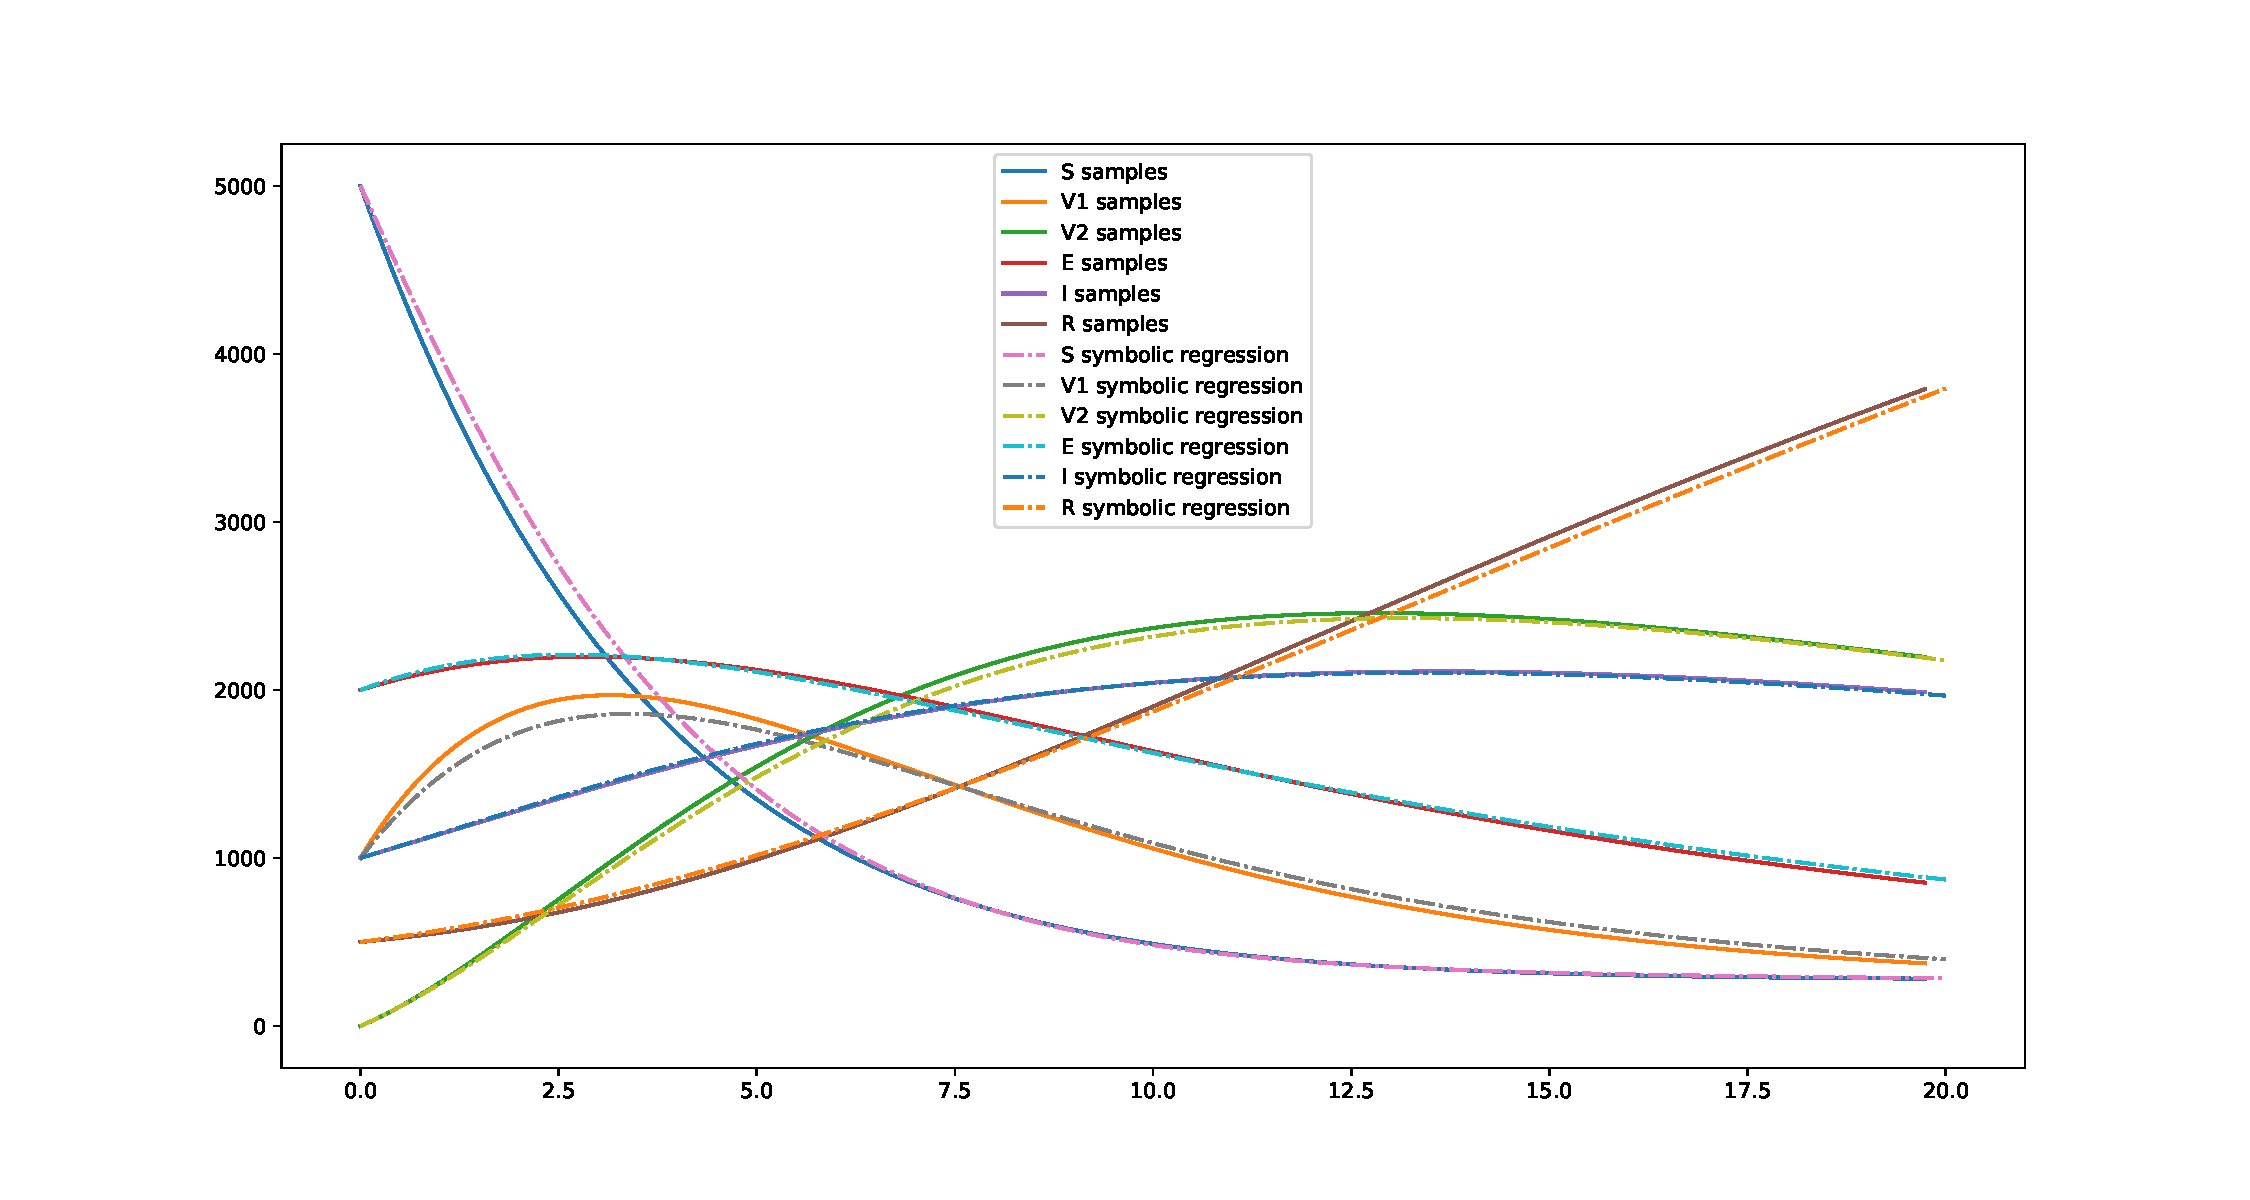
\includegraphics[width=\textwidth]{"figures/final_plot_SVVEIR_0.05.pdf"}
    \caption{Modelo resultante utilizando datos generados a partir del modelo SVVEIR con ruido máximo de 5\%.}
    \label{fig:final_plot_SVVEIR_0.05}
\end{figure}

\begin{figure}[h]
    \centering
    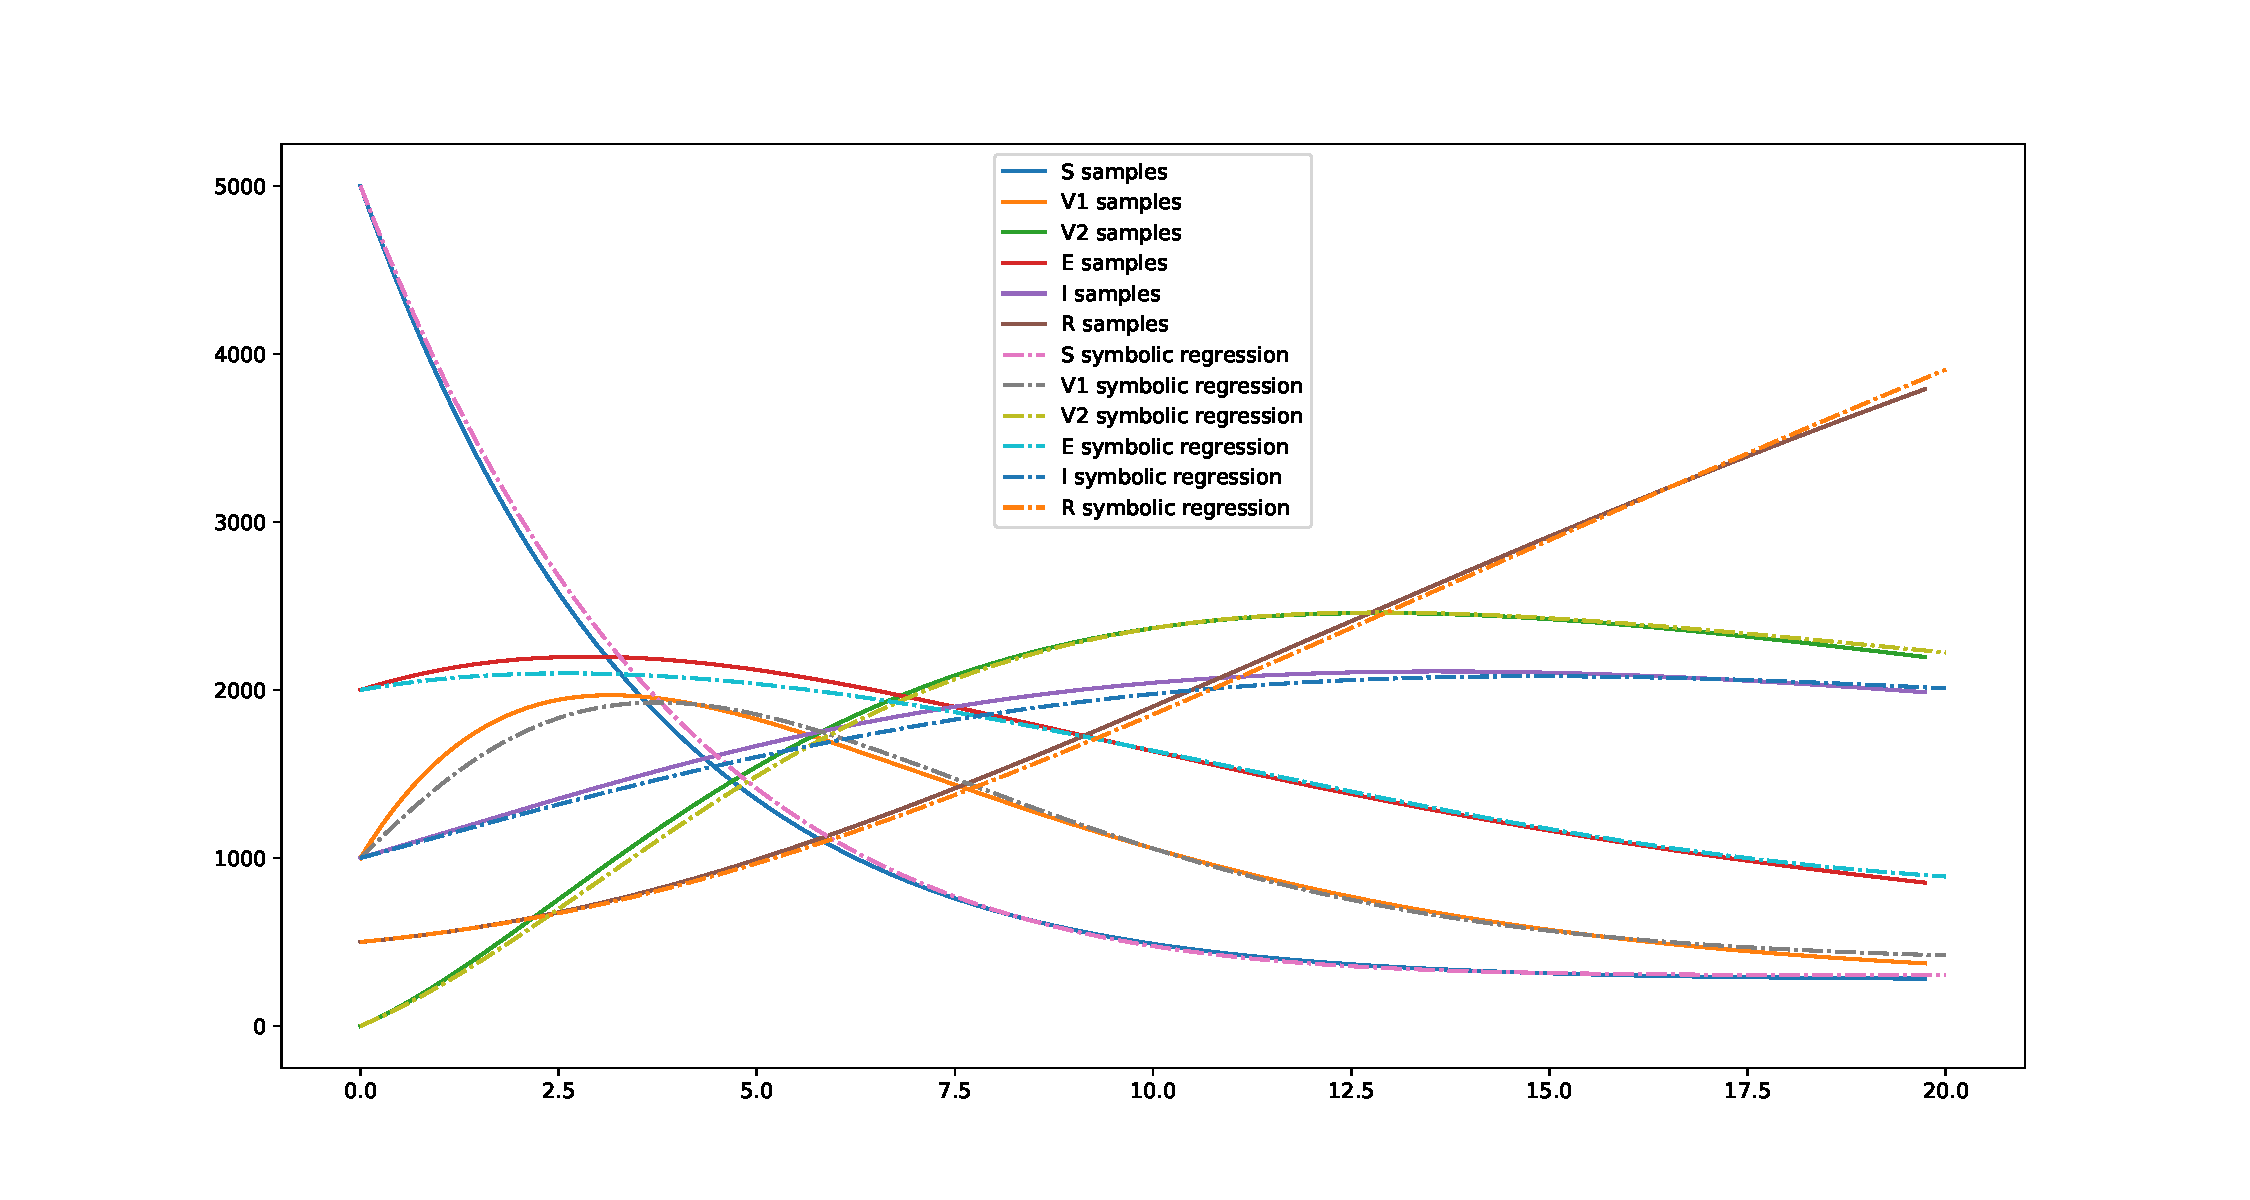
\includegraphics[width=\textwidth]{"figures/final_plot_SVVEIR_0.1.pdf"}
    \caption{Modelo resultante utilizando datos generados a partir del modelo SVVEIR con ruido máximo de 10\%.}
    \label{fig:final_plot_SVVEIR_0.1}
\end{figure}

Si en lugar de utilizar como aproximación el método de diferencias finitas cuando los datos no poseen ruido, se utiliza el sistema original de SIR, se obtiene que la media del valor de la función de ajuste a lo largo de las 30 ejecuciones del experimento es $3.68731$. El valor máximo de la función de ajuste alcanzado fue de $19.45527$ y el mínimo de $0.58707$, en este último la regresión simbólica no obtuvo el sistema original.

En la siguiente sección se realiza un análisis de los resultados de todos los experimentos realizado.

\section{Análisis de resultados}\label{section:experiments_results}

Los resultados obtenidos durante los experimentos muestran que la regresión simbólica planteada puede encontrar un sistema $f_{aprox}$ que ajuste los datos $y'_{original}$ generados a partir de la derivada aproximada por el método de diferencias finitas sobre los datos $y_{original}$ donde $y_{original}$ son los datos obtenidos de la integración del sistema conocido $f$.

Al generar el conjunto $y_{noise}$ a partir de agregar ruido a $y_{original}$ que describen la función $y$, no se puede aproximar la derivada de $y$ por el método de diferencias finitas. La función $y$ se aproxima utilizando un spline de suavizado cúbico sobre $y_{noise}$ obteniéndose los datos $y_{spline}$. Del spline de suavizado se puede obtener el valor de la primera derivada y así generar el conjunto $y'_{spline}$. Al utilizar los valores de $y_{spline}$ y $y'_{spline}$ en el método de regresión simbólica se obtiene el sistema $f_{aprox_{sr}}$.

El error cuádratico médio de los datos $y_{spline}$ evaluados en el sistema $f_{aprox_{sr}}$ es mayor que el de los datos $y_{original}$ evaluados en el sistema $f_{aprox}$. Mientras mayor el ruido presente en $y_{noise}$ mayor es la diferencia entre los valore del ajuste.

Si se integra el sistema $f_{aprox}$ se obtiene el conjunto de puntos $y_{aprox}$. El valor del error cuádratico medio entre los conjuntos $y_{aprox}$ y $y_{original}$ es menor en los sistemas que no poseen términos con un parámetro sin estar multiplicando una expresión.

Si se definen los datos $y_{aprox_{sr}}$ como el resultado de la integración del sistema $f_{aprox_{sr}}$, se puede analizar como el error cuadrático medio entre los puntos $y_{aprox_{sr}}$ y $y_{spline}$ es igual que el error cuádratico medio entre los puntos $y_{aprox_{sr}}$ y $y_{original}$.

En los sistemas con menos de 6 ecuaciones, los resultados de aplicar la restricción de las variables que pueden existir en cada ecuación son semejantes a los resultados obtenidos sin aplicar la restricción.

En los experimentos utilizando los modelos SIR, SIRD, SIQRD y SVVEIR nunca se obtuvo el sistema original como resultado de la regresión simbólica, sin embargo si se obtuvieron sistemas que fueron capaces de ajustar los datos con valores en la función de ajuste cercanos a 0.

La utilización del modelo original para la aproximación de $y'_{original}$ hace que se obtengan los resultados con el menor valor de ajuste, obtiéndose exactamente el sistema original en algunos experimentos correspondientes a los modelos Lotka-Volterra, SIR, SIRD y SIQRD.

\backmatter

\chapter*{Conclusiones}\label{chapter:conclusions}
\addcontentsline{toc}{chapter}{Conclusiones}

En este trabajo se diseño e implementó un sistema de regresión simbólica basada en algoritmos genéticos para encontrar un sistema de ecuaciones diferenciales lineales con respecto a los parámetros en el que es posible determinar qué variables intervienen en cada ecuación.

Con este fin se definió cómo representar los sistemas de ecuaciones diferenciales en forma de árbol computacional de manera que solo se permitiese representar sistemas lineales con respecto a los parámetros. Para el uso del algoritmo genético se definieron las operaciones de mutación, cruzamiento y selección sobre estos árboles. Además se utilizó un spline de suavizado para eliminar el ruido en los datos.

Se utilizó la propiedad de linealidad con respecto a los parámetros de los sistemas de ecuaciones para ajustar los parámetros en cada solución resolviendo un sistema de ecuaciones lineales.

Para probar el funcionamiento del sistema creado se utilizaron datos generados a partir de 5 sistemas de ecucaciones diferenciales conocidos, comprobándose así la calidad de las soluciones obtenidas por la regresión simbólica.
\begin{recomendations}

    Los parámetros utilizados en el algoritmo genético empleado en la regresión simbólica fueron los mismos en cada experimento, se recomienda hacer un estudio de la selección de estos parámetros.

    Para impedir que árboles con más de $k$ niveles se puedan obtener, se propone modificar las operaciones de mutación y cruzamiento, siendo $k$ otro parámetro que se puede incorporar al algoritmo genético.

    Como trabajo futuro se puede estudiar la cantidad de muestras sin ruido mínimas necesarias para obtener exactamente el sistema que originó los datos.

    Buscar formas de lidiar con los sistemas con grandes expresiones, como la división presente en la primera y segunda ecuación del sistema SIRD.

\end{recomendations}

\nocite{*}
\bibliographystyle{plain}
\bibliography{Bibliography}
\end{document}